%%%%%%%%%%%%%%%%%%%%%%%%%%%%%%%%%%%%%%%%%%%%%%%%%%%%%%%%%%%%%%%%%%%%%%%%%%%%%%%
%% Copyright (c) 2010, 2024 Contributors to the Eclipse Foundation
%%
%% See the NOTICE file(s) distributed with this work for additional
%% information regarding copyright ownership.
%%
%% This program and the accompanying materials are made available under the terms
%% of the MIT License which is available at https://opensource.org/licenses/MIT
%%
%% SPDX-License-Identifier: MIT
%%%%%%%%%%%%%%%%%%%%%%%%%%%%%%%%%%%%%%%%%%%%%%%%%%%%%%%%%%%%%%%%%%%%%%%%%%%%%%%

\PassOptionsToPackage{usenames,dvipsnames}{xcolor}

\documentclass{report}

% General used packages.
\usepackage[a4paper]{geometry}
\usepackage[final]{pdfpages}

% For generating hyper-references
\usepackage{hyperref}
\usepackage{verbatim}
\usepackage{color}
\usepackage{amssymb}
\usepackage{amsmath}
\usepackage{stmaryrd}
\usepackage{import}
\usepackage{subfig}

% For title page image
\usepackage{titlepic}
\usepackage{graphicx}

% For figure 'H' placement
\usepackage{float}

% yes (green tick) and no (red cross) commands
\usepackage{amsfonts}
\newcommand{\yes}{\textcolor{Green}{\hspace{2pt}\checkmark}}
\usepackage{pifont}
\newcommand{\no}{\textcolor{red}{\ding{55}}}

% tikz
\usepackage{tikz}
\usetikzlibrary{arrows,automata,petri,fit} % positioning

% CIF commands.
\newcommand{\cifpkg}[1]{\textit{#1} (Section~\ref{cifpkg:#1})}
\newcommand{\cifclass}[1]{\textit{#1} (Section~\ref{cifclass:#1})}
\newcommand{\cifattr}[1]{\textit{#1} (Section~\ref{cifattr:#1})}
\newcommand{\cifenumlit}[1]{\textit{#1} (Section~\ref{cifenumlit:#1})}
\newcommand{\cifclassDetail}[7]{\item {#1} \textbf{#2} {#3} :
   {\textit{#4}} {#5} {#6} \hfill \\ {#7}}
\newcommand{\cifenumlitDetail}[4]{\item literal \textbf{#1} {#2} {#3}
   \hfill \\ {#4}}

% Position commands.
\newcommand{\positionpkg}[1]{\textit{#1} (Section~\ref{positionpkg:#1})}
\newcommand{\positionclass}[1]{\textit{#1} (Section~\ref{positionclass:#1})}
\newcommand{\positionattr}[1]{\textit{#1} (Section~\ref{positionattr:#1})}
\newcommand{\positionenumlit}[1]{\textit{#1} (Section~\ref{positionenumlit:#1})}
\newcommand{\positionclassDetail}[7]{\item {#1} \textbf{#2} {#3} :
   {\textit{#4}} {#5} {#6} \hfill \\ {#7}}
\newcommand{\positionenumlitDetail}[4]{\item literal \textbf{#1} {#2} {#3}
   \hfill \\ {#4}}

% Hook commands.
\newcommand{\hook}{\hspace*{5pt}\raisebox{2.5pt}{$\llcorner$}}
\newcommand{\hookindent}{\hspace*{15pt}}

% Constraint commands.
\newenvironment{constraints}{Constraints:\begin{itemize}}{\end{itemize}}
\newcommand{\citem}[1]{\item \textbf{#1}}
\newcommand{\citemnf}[1]{\item \textbf{#1 (non-fatal)}}

% Layout settings.
\setlength{\parindent}{0pt}
\setlength{\parskip}{1.5ex}

% Ranges.
\newcommand{\range}[2]{$[{#1}~..~{#2}]$}
\newcommand{\rangeBig}[2]{$\left[~{#1}~..~{#2}~\right]$}
\newcommand{\mathrange}[2]{[{#1}~..~{#2}]}
\newcommand{\rangeV}[2]{$\left[
                         \begin{array}{@{}l@{\,}l@{}}
                           ~{#1} & ..~ \\
                           ~{#2} &   ~ \\
                         \end{array}
                        \right]$}


% Todo command.
% \newcommand{\todo}[1]{\textcolor{red}{#1}}
%\newcommand{\todo}[1]{}

% \newcommand{\question}[1]{\textcolor{orange}{#1}}
%\newcommand{\question}[1]{}

% Ecore language name.
\newcommand{\ecorelang}{CIF}

% Document settings.
\title{CIF Metamodel Reference Documentation}
\author{Copyright (c) 2010, 2024 Contributors to the Eclipse Foundation}
\date{Version 2024-05-10}

% Start of document.
\begin{document}
\maketitle
\tableofcontents

%%%%%%%%%%%%%%%%%%%%%%%%%%%%%%%%%%%%%%%%%%%%%%%%%%%%%%%%%%%%%%%%%%%%%%%%%%%%%%%
\chapter{Introduction}
CIF is a declarative modeling language for the specification of discrete
event, timed, and hybrid systems as a collection of synchronizing automata.
The CIF tooling supports the entire development process of controllers,
including among others specification, supervisory controller synthesis,
simulation-based validation and visualization, verification, real-time
testing, and code generation.

CIF is one of the tools of the Eclipse ESCET\textsuperscript{\texttrademark{}}
project~\cite{Eclipse:ESCET}.

\import{../../../common/org.eclipse.escet.common.position.metamodel/docs/}
       {ecore_intro.tex}

This report is organized as follows. The notations and conventions used in
this document are explained in Chapter~\ref{ch:notations-conventions},
Chapter~\ref{ch:cif} describes the CIF metamodel, and
Chapter~\ref{ch:distributions} describes the stochastic distributions in more
detail.


%%%%%%%%%%%%%%%%%%%%%%%%%%%%%%%%%%%%%%%%%%%%%%%%%%%%%%%%%%%%%%%%%%%%%%%%%%%%%%%
\chapter{Notations and conventions}\label{ch:notations-conventions}

\section{Ecore class diagrams}

\import{../../../common/org.eclipse.escet.common.position.metamodel/docs/}
       {ecore_diagrams.tex}

For the CIF language, arrows colored in red are containments, but should
be interpreted semantically as references. That is, in order to allow
wrapping expressions and types to be used, they are containments instead of
references. See also Section~\ref{sec:scoping}.


\section{Metamodel documentation conventions}

\import{../../../common/org.eclipse.escet.common.position.metamodel/docs/}
       {ecore_doc_conventions.tex}


%%%%%%%%%%%%%%%%%%%%%%%%%%%%%%%%%%%%%%%%%%%%%%%%%%%%%%%%%%%%%%%%%%%%%%%%%%%%%%%
\chapter{CIF metamodel}\label{ch:cif}

The CIF metamodel consists of the following packages:
\begin{itemize}
    \item \emph{cif} package: includes component structure and component
        definition/instantiation (Section~\ref{cifpkg:cif} at
        page~\pageref{cifpkg:cif}),
    \item \emph{declarations} sub-package: includes CIF declarations,
        including among others events and variables
        (Section~\ref{cifpkg:declarations} at
        page~\pageref{cifpkg:declarations}),
    \item \emph{automata} sub-package: includes automata, the basic components
        of CIF models (Section~\ref{cifpkg:automata} at
        page~\pageref{cifpkg:automata}),
    \item \emph{types} sub-package: includes CIF types
        (Section~\ref{cifpkg:types} at page~\pageref{cifpkg:types}),
    \item \emph{expressions} sub-package: includes CIF expressions
        (Section~\ref{cifpkg:expressions} at
        page~\pageref{cifpkg:expressions}),
    \item \emph{functions} sub-package: includes internal and external
        user-defined CIF functions (Section~\ref{cifpkg:functions} at
        page~\pageref{cifpkg:functions}),
    \item \emph{cifsvg} sub-package: includes CIF/SVG I/O declarations
        (Section~\ref{cifpkg:cifsvg} at page~\pageref{cifpkg:cifsvg}),
    \item \emph{print} sub-package: includes print I/O declarations
        (Section~\ref{cifpkg:print} at page~\pageref{cifpkg:print}),
    \item \emph{annotations} sub-package: includes annotations
        (Section~\ref{cifpkg:annotations} at page~\pageref{cifpkg:annotations}),
        and
    \item \emph{position} package: position information
        (Section~\ref{positionpkg:position} at
        page~\pageref{positionpkg:position}).
\end{itemize}

The class diagrams are presented and described in the respective sections
below.

Note that the \textit{position} package is not actually part of the CIF
metamodel. It is actually part of the \textit{position} metamodel, but it is
used by the CIF metamodel to represent position information. As such, the
documentation for the \textit{position} package is included in this document,
for completeness. All CIF classes directly or indirectly derive from
\positionclass{PositionObject}.


\section{Scoping}\label{sec:scoping}

\subsection{Reference wrapping}\label{sec:ref-wrapping}

One of the features of CIF is that pretty much anything in the entire
specification can be referenced from anywhere in the specification. This
is however complicated by the existence of a component
definition/instantiation mechanism.

\begin{figure}[!ht]
  \centering
  \subfloat[The model]{
    \label{fig:wrapping-pre-model}
    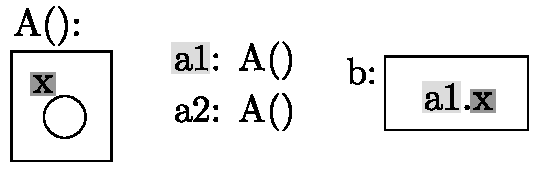
\includegraphics[width=0.45\textwidth]{figures/wrapping_pre_model.pdf}
  }
  \hfill
  \subfloat[The reference expression]{
    \label{fig:wrapping-pre-expr}
    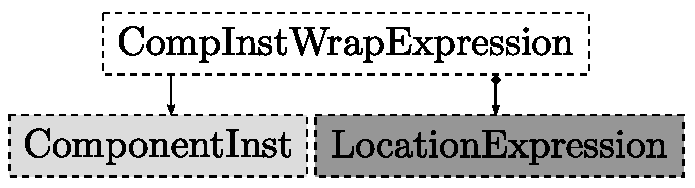
\includegraphics[width=0.45\textwidth]{figures/wrapping_pre_expr.pdf}
  }
  \caption{Wrapping expression example: situation before.}
  \label{fig:wrapping-pre}
\end{figure}

Take a look at Figure~\ref{fig:wrapping-pre-model}. It shows a CIF model with
a component definition \texttt{A}, which contains a location \texttt{x}. This
component definition is instantiated twice, once as \texttt{a1}, and once as
\texttt{a2}. Finally, there is a component \texttt{b}, which refers to
location \texttt{x} of component \texttt{a1}. The reference
is written in the CIF textual syntax.

Figure~\ref{fig:wrapping-pre-expr} shows the corresponding instance of
metamodel classes that is generated by the compiler to represent the
\texttt{a1.x} text. Instead of just generating a reference to an instance
of the \cifclass{Location} class, an expression is used. An instance of the
\cifclass{LocationExpression} class is wrapped in an instance of
the \cifclass{CompInstWrapExpression} class, which also references an
instance of the \cifclass{ComponentInst} class.

What we see here is a direct representation of the textual syntax, as we
reference location \texttt{x} via component instantiation \texttt{a1}. We
need to keep track
of references via component instantiations. If we were to only generate an
instance of the \cifclass{LocationExpression} class, or just use a direct
reference to an instance of the \cifclass{Location} class, we would no
longer be able to distinguish between location \texttt{x} in component
\texttt{a1}, and location \texttt{x} in component \texttt{a2}.

\begin{figure}[!ht]
  \centering
  \subfloat[The model]{
    \label{fig:wrapping-post-model}
    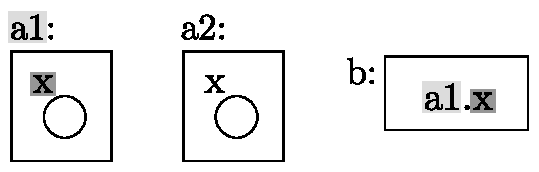
\includegraphics[width=0.45\textwidth]{figures/wrapping_post_model.pdf}
  }
  \hfill
  \subfloat[The reference expression]{
    \label{fig:wrapping-post-expr}
    
\includegraphics[width=0.45\textwidth]{figures/wrapping_post_expr.pdf}
  }
  \caption{Wrapping expression example: situation after.}
  \label{fig:wrapping-post}
\end{figure}

Figure~\ref{fig:wrapping-post-model} shows the model after elimination of
component definition/instantiation. We see that components instantiations
\texttt{a1} and \texttt{a2} are replaced by components \texttt{a1} and
\texttt{a2}, which are essentially equal to the body of component definition
\texttt{A}. As such, we now have two locations \texttt{x}, one in component
\texttt{a1}, and one in component \texttt{a2}. The text to refer to location
\texttt{x} of component \texttt{a1}, as used in component \texttt{b}, is
still \texttt{a1.x}.

Figure~\ref{fig:wrapping-post-expr} shows the corresponding reference
expression. It is no longer necessary to use a wrapping expression, as we
can refer to location \texttt{x} in component a1 directly, as it is a real
location, not one that we can get multiple versions of due to instantiation.
As such, there is no confusion about which location we mean by that reference
expression.

Note that wrapping does not only apply to references via component
instantiations, but also to references via component parameters.
Also, it does not just apply to expressions references, but also to type
references. See also the \cifclass{CompInstWrapType},
\cifclass{CompParamWrapType}, \cifclass{CompInstWrapExpression}, and
\cifclass{CompParamWrapExpression} classes.

From this we can conclude that reference expressions, reference types, and
their wrapping variants, are necessary to keep track of the component
instantiations and component parameters via which we reference certain
objects. That is, we need to correctly capture all of the information contained
in the textual representations of references, in our metamodel representation.
This is for instance needed to be able to correctly reroute references during
the elimination of component definition/instantiation. After that elimination
step however, wrapping expressions and wrapping types are no longer present.
References do remain expressions, and as such, in the example, an instance
of the \cifclass{LocationExpression} is contained, instead of a direct
reference to an instance of the \cifclass{Location} class. Such containments
are colored in red in the metamodel, as already mentioned in
Chapter~\ref{ch:notations-conventions}.


\subsection{Scoping rules}

As previously mentioned in Section~\ref{sec:ref-wrapping}, one of the features
of CIF is that pretty much anything in the entire specification can be
referenced from anywhere in the specification. This is however complicated by
the existence of a component definition/instantiation mechanism, which caused
a need for reference wrapping.

This section explains the scoping rules of CIF.
Figure~\ref{fig:scoping-visibility} shows an example CIF specification. The
rectangles in the figure indicate components and component definitions. The
outer rectangle (the dashed one), indicates the entire specification. The
text fragments are written in a slightly simplified version of the CIF textual
syntax. In the remainder of this section, the example is used to explain
the scoping rules.

\begin{figure}
  \centering
  \import{figures/}{scoping_visibility.tex}
  \caption{Scoping and visibility example.}
  \label{fig:scoping-visibility}
\end{figure}

The first thing to note about the figure are the different colors. They
indicate the different scopes of the specification. The outer-most scope (the
red scope) is the specification scope. We walk the containment hierarchy
downwards until we hit a component definition. From there, we start a new
scope, and repeat the process. That is, specifications and component
definitions start a new scope. The idea is that component definitions are
definitions, and as such we can't refer to objects in component definitions
directly. If we were to be able to reference objects in component definitions
directly, and there would not be any instance of such a component definition,
or there would be multiple instances, to what would we be referring? So, to
solve this ambiguity, only once we instantiate a component definition, can we
refer to objects within that definition (via component instantiation reference
wrapping expressions for instance).

An example of this is component
instantiation \texttt{c:} \texttt{C()} in component \texttt{a}. In component
\texttt{a}, in the red scope, we can't directly reference objects from
component definition \texttt{C}, as those objects are in the green scope. Once
we have \texttt{c}, we can use it to refer to objects in \texttt{C}, such
as \texttt{c.b}. In fact, \texttt{c.b.a.a.x} refers to location \texttt{x}
(black scope) in component \texttt{a.a} (black scope) in component definition
\texttt{B}, via component instantiations \texttt{c} (red scope to green scope)
and \texttt{b} (green scope to black scope).

Note how a component definition itself is part of the enclosing scope, while
the parameters are part of the new scope that is introduced by the component
definition. That is, the parameter cannot be referenced directly from the
enclosing scope. If we look at component definition \texttt{K}, we see that
component parameter \texttt{c} is part of the new blue scope. The type of
component parameter \texttt{c} is component \texttt{C}, which is resolved
in the enclosing scope (the red scope).

Within a single scope (single color in the figure), anything can be referenced
directly. For instance, in component \texttt{a} (red scope), references
\texttt{b.x} and \texttt{b.y} refer to locations in automaton \texttt{b},
which is part of the same red scope. Furthermore, component definition
\texttt{P} (from component \texttt{i}) can be instantiated directly in
component \texttt{a}, as both are in the red scope.

In general, anything within the same scope can be referenced directly, as can
anything from ancestors scopes (the parent scope, the parent of the parent
scope, etc). An example of the latter is \texttt{d.x}
in an invariant of component \texttt{C.B.a} (in the black scope), which refers
to location \texttt{C.d.x} of automaton \texttt{C.d}, in the green parent
scope. The only two ways to reference things in component definitions
that the reference itself is not a part of, are via component
instantiations and via component parameters. For an example of the latter,
see invariant \texttt{inv c.d.x} in component definition \texttt{K}.

Note that it is not allowed to instantiate component definitions which, in the
instantiation context, can only be referenced via another component
instantiation or via a component parameter. That is, it is not allowed to
instantiate a component definition X, declared inside other component
definition Y, from outside Y. Conceptually, in an instantiated component,
there are no component definitions.

Also, it is not allowed to refer to a parameter of a component definition,
via component instantiations or via other component parameters. Once again,
conceptually, in an instantiated component, there are no parameters.

For user-defined functions, it is not allowed to refer to anything inside a
function (parameters etc) from outside the function. The other way around, from
inside a function, it is not allowed to refer to variables, locations, events,
components, component definitions, etc. Objects with constant values (such as
constants etc) may be referenced from inside functions, as may types (type
declarations, enumerations, etc).

The scoping rules for tuple fields are special. See the
\cifclass{ProjectionExpression} class for further details.


\subsection{Visibility}

Within the metamodel, the scoping rules are enough. However, in the CIF
textual syntax, the concept of \emph{visibility} is important as well.

If we look at Figure~\ref{fig:scoping-visibility}, we see that relative
references to objects that are `in scope' are possible. For instance, in
component \texttt{a}, there is a relative reference to \texttt{b.x}.
Reference \texttt{c.b.a.a.x} is a relative reference as well, even though it
uses some component instantiations to reach other scopes. Relative references
refer to objects in the same sub-scope or deeper sub-scopes, possibly via
references to other scopes.

Relative references are also possible to objects defined at higher levels,
as for instance shown by discrete variable \texttt{C.B.a.a.v0}, which has type
\texttt{t}. This type \texttt{t} is defined one sub-scope above, in
\texttt{C.B.a}.

The other discrete variables in that same automaton, discrete variables
\texttt{v1} and
\texttt{v2}, also have type \texttt{t} as their type, but refer to different
types \texttt{t}. Since only one object with a given name can be visible in
a scope or sub-scope, types \texttt{t} (in the specification scope) and
\texttt{C.B.t} are not visible in automaton \texttt{C.B.a.a}. They are however
`in scope', as they are type declarations in the same scope or in ancestor
scopes.

To be able to refer to objects that are in scope, but are \emph{hidden} by
other declarations of the same name, absolute references can be used. There
are two variants: scope absolute references and specification absolute
references. The type \texttt{.t} of discrete variable \texttt{v1} is a scope
absolute
reference. The reference starts with a single dot (\texttt{.}) and is then
relative to the root of the current scope (the black scope). The type
\texttt{\^{}t} of discrete variable \texttt{v2} is a specification absolute
reference. The reference starts with a caret (\texttt{\^}) and is then
relative to the root of the current specification (the red scope).

Note that functions, similar to components, introduce a sub-scope.

Note that tuple projection expressions may introduce a sub-scope. This scope has
the tuple fields as objects. This kind of sub-scope is special in the sense that
the fields are only in scope of the projection expression. Note that as for all
scopes, fields may hide other objects with the same name, from parent scopes.
Note that if it is a field reference, the textual reference to that field must be
a single identifier. For instance, for a tuple-typed variable \texttt{t},
\texttt{t[i]} can be a field reference but \texttt{t[i + 1]} can not. If the
index expression is a reference to another object that can be referred to by a
single identifier, then that object may be hidden by a tuple field with that same
name. In such cases the object can't be referred to by a single identifier as the
field name takes precedence, hiding the object. A more complex textual reference,
such as a scope absolute reference, must then be used instead to refer to the
object.

%%%%%%%%%%%%%%%%%%%%%%%%%%%%%%%%%%%%%%%%%%%%%%%%%%%%%%%%%%%%%%%%%%%%%%%%%%%%%%%
\newpage

\import{../../../common/org.eclipse.escet.common.position.metamodel/docs/}
       {position_ecore_doc_details.tex}
%%%%%%%%%%%%%%%%%%%%%%%%%%%%%%%%%%%%%%%%%%%%%%%%%%%%%%%%%%%%%%%%%%%%%%%%%%%%%%%
%% Copyright (c) 2010, 2024 Contributors to the Eclipse Foundation
%%
%% See the NOTICE file(s) distributed with this work for additional
%% information regarding copyright ownership.
%%
%% This program and the accompanying materials are made available under the terms
%% of the MIT License which is available at https://opensource.org/licenses/MIT
%%
%% SPDX-License-Identifier: MIT
%%%%%%%%%%%%%%%%%%%%%%%%%%%%%%%%%%%%%%%%%%%%%%%%%%%%%%%%%%%%%%%%%%%%%%%%%%%%%%%

%%%%%%%%%%%%%%%%%%%%%%%%%%%%%%%%%%%%%%%%%%%%%%%%%%%%%%%%%%%%%%%%%%%%%%%%%%%%%%%
% Package cif
%%%%%%%%%%%%%%%%%%%%%%%%%%%%%%%%%%%%%%%%%%%%%%%%%%%%%%%%%%%%%%%%%%%%%%%%%%%%%%%
\newcommand{\pkgdocucif}{
\begin{figure}
  \centering
  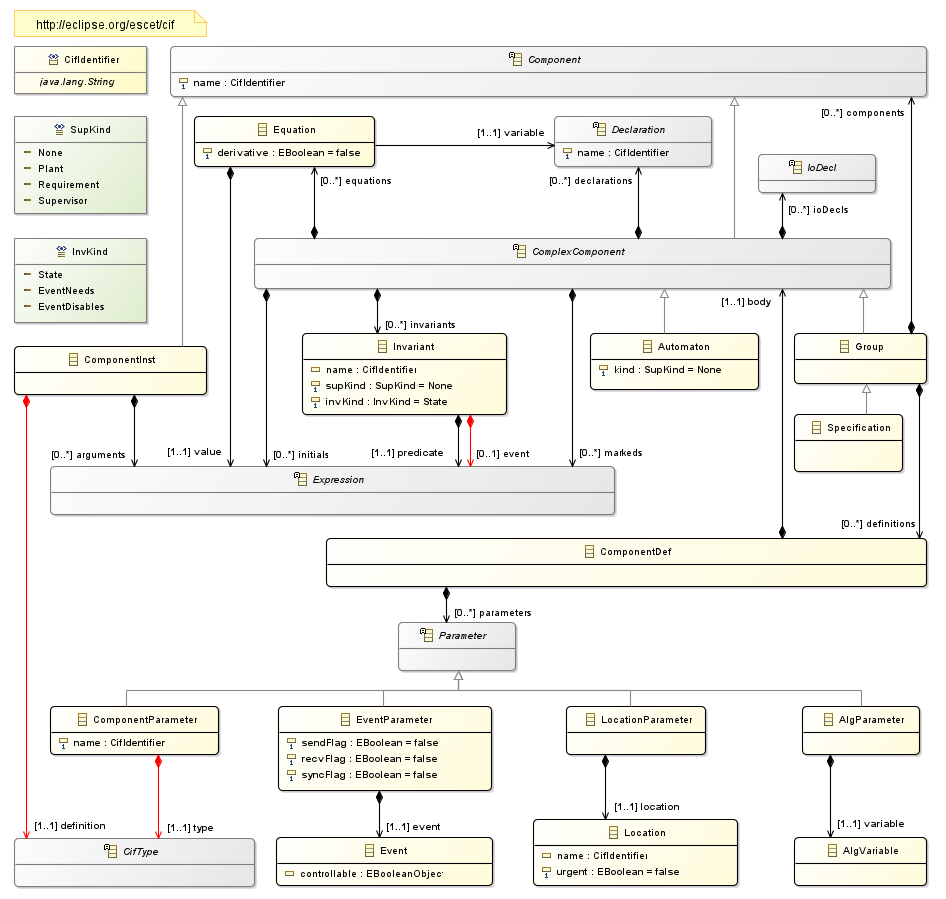
\includegraphics[width=\textwidth]{../model/images/cif.png}
  \caption{\textit{cif} package}\label{fig:pkg:cif}
\end{figure}

Figure~\ref{fig:pkg:cif} shows the \textit{cif} package.
This package contains classes that are used to represent the component
structure of CIF models. It also includes the component
definition/instantiation related classes.

The \cifclass{Component} class represents CIF components. There are three
types of components: automata (\cifclass{Automaton} class), groups
(\cifclass{Group} class), and component instantiations
(\cifclass{ComponentInst} class). Automata and groups share a common
base class (\cifclass{ComplexComponent}), since they share many features.
The root object of every CIF model is an instance of the
\cifclass{Specification} class, a special form of \cifclass{Group}.

The bottom part of the \textit{cif} package diagram deals with component
definitions (\cifclass{ComponentDef} class) and their parameters.
}

% CifIdentifier (datatype)
\newcommand{\dtypedocuCifIdentifier}{
A CIF identifier starts with a letter or an underscore character, and is
followed by zero or more letters, digits, and/or underscore characters.

Note that it is allowed to use keywords from the textual syntax as identifiers.
In the CIF textual syntax, this is allowed as well, but requires that the
keyword is prefixed with a dollar sign (\texttt{\$}). This prefix is not
allowed in the metamodel, as there is no ambiguity.
}

% InvKind (enumeration)
\newcommand{\enumdocuInvKind}{
Invariant kind. Indicates whether an invariant is a state (exclusion) invariant
or a state/event exclusion invariant, and for state/event exclusion invariants
also in what form it is written.
}

\newcommand{\enumlitdocuInvKindEventDisables}{
A state/event exclusion invariant, giving a sufficient condition for an event
to be disabled. A predicate and event are given with the invariant. The event
is disabled in states where the predicate holds. If the predicate does not
hold in a state, the event may or may not be enabled, depending on the
automata and other (invariant) restriction of the system.
}

\newcommand{\enumlitdocuInvKindEventNeeds}{
A state/event exclusion invariant, giving a necessary condition for an event
to be enabled. A predicate and event are given with the invariant. The event
is only enabled in states where the predicate holds. More precisely, if the
predicate does not hold in a state, the event is disabled.
}

\newcommand{\enumlitdocuInvKindState}{
A state (exclusion) invariant. A predicate is given with the invariant that
indicates which states are allowed. All states not satisfying the predicate
may never be active states, i.e. may never be reached.
}

% SupKind (enumeration)
\newcommand{\enumdocuSupKind}{
Supervisory kind. Indicates how an automaton or invariant is to be
interpreted for supervisory synthesis and related algorithms/tools.
}

\newcommand{\enumlitdocuSupKindNone}{
Regular automaton or invariant. Indicates that the kind is considered
irrelevant (it is just an automaton or invariant, nothing else). This kind is
usually used if the automaton or invariant is not to be used for synthesis,
verification, etc.
}

\newcommand{\enumlitdocuSupKindPlant}{
Plant automaton or invariant. A plant automaton specifies the behavior of
the uncontrolled physical system, or a part of it. Plant automata may abstract
away from details of the actual physical system, if those details are
considered irrelevant. A plant invariants restricts the behavior of the
uncontrolled physical system, or a part of it.
}

\newcommand{\enumlitdocuSupKindRequirement}{
Requirement automaton or invariant. A requirement automaton or invariant (or
requirement) represents the required behavior of the controlled system, or a
part of it. Requirements can be synthesized, verified, etc.
}

\newcommand{\enumlitdocuSupKindSupervisor}{
Supervisor automaton or invariant. A supervisor automaton (or supervisor) can
be used to control the uncontrolled plant. A supervisor invariant restricts the
behavior of the supervised system, or a part of it.
}

% AlgParameter (class)
\newcommand{\clsdocuAlgParameter}{
An algebraic (variable) parameter of a \cifclass{ComponentDef}.

Note that there are no constant parameters. However, constants may be provided
as arguments for algebraic parameters.
}

\newcommand{\featdocuAlgParametervariable}{
The algebraic variable declaration that represents the algebraic parameter.

\begin{constraints}
\citem{AlgParameter.noValue}
  The \emph{variable} declaration must not have a value, since the argument
  should provide it.
\end{constraints}
}

% ComplexComponent (abstract class)
\newcommand{\clsdocuComplexComponent}{
Base class for more complex components. That is, for components that have
declarations etc. This class was introduced to allow sharing of structural
features between the \cifclass{Automaton} and \cifclass{Group} classes.
% NOTE: unique name constraint in derived classes instead of this class.
}

\newcommand{\featdocuComplexComponentdeclarations}{
The declarations of the component.
}

\newcommand{\featdocuComplexComponentequations}{
The equations of the component.
}

\newcommand{\featdocuComplexComponentinitials}{
The initialization predicates of the component. A CIF model can only start
in states that satisfy the initialization predicates.

If no predicates are given, the initialization predicate is \emph{true}. If
multiple predicates are given, this feature represents the logical conjunction
of those predicates. Note that this represents the mathematical conjunction,
and not the short-circuit conjunction binary operator. As such, there is
no ordering between initialization predicates.

See the documentation of the derived classes for information on how to
combine the initialization predicates with other levels.

\begin{constraints}
\citem{ComplexComponent.initialTypes}
  The initialization predicates must have boolean types.
\end{constraints}
}

\newcommand{\featdocuComplexComponentinvariants}{
The invariants of the component. A CIF model can only be in a state
if that state satisfies the invariants.

If no invariants are given, the invariant is \emph{true}. If multiple
invariant are given, this feature represents the logical conjunction
of those invariants. Note that this represents the mathematical conjunction,
and not the short-circuit conjunction binary operator. As such, there is
no ordering between invariants.

See the documentation of the derived classes for information on how to
combine the invariants with other levels.
}

\newcommand{\featdocuComplexComponentioDecls}{
The I/O declarations of the component.

\begin{constraints}
\citem{ComplexComponent.maxOneSvgFile}
  Must not contain more than one \cifclass{SvgFile} declaration.
\citem{ComplexComponent.maxOnePrintFile}
  Must not contain more than one \cifclass{PrintFile} declaration.
\end{constraints}
}

\newcommand{\featdocuComplexComponentmarkeds}{
The marker predicates of the component. Used as liveness property for, among
others, supervisory controller synthesis.

If no predicates are given, the marker predicate is \emph{true}. If
multiple predicates are given, this feature represents the logical conjunction
of those predicates. Note that this represents the mathematical conjunction,
and not the short-circuit conjunction binary operator. As such, there is
no ordering between marker predicates.

See the documentation of the derived classes for information on how to
combine the marker predicates with other levels.

\begin{constraints}
\citem{ComplexComponent.markedTypes}
  The marker predicates must have boolean types.
\end{constraints}
}

% Component (abstract class)
\newcommand{\clsdocuComponent}{
Base class of all CIF components. Components model the structure of a CIF
model.
}

\newcommand{\featdocuComponentname}{
The name of the component.

\begin{constraints}
\citemnf{Component.name}
  Component names must not start with \texttt{e\_}, \texttt{c\_}, or
  \texttt{u\_}, as those prefixes are reserved for events.
\end{constraints}
}

% ComponentDef (class)
\newcommand{\clsdocuComponentDef}{
A component definition. Component definitions allow reuse of components. They
can be instantiated using a \cifclass{ComponentInst}. Note that component
definitions are not components themselves. They must be instantiated to
become actual components.

In the metamodel, the \emph{ComponentDef} class itself is just a wrapper that
has parameters and a body. The name of the body defines the name of the
component definition. The body is considered a part of the component
definition, and as such, the body (component) may not be referenced directly.

If we eliminate a component definition, the instantiation is replaced by the
body of the component definition, all reference parameters are substituted in
the body (which has become an actual component), and algebraic parameters
become local algebraic variables in that component (the body).

\begin{constraints}
\citem{ComponentDef.uniqueDecls}
  The names of all parameters, as well as the declarations and invariants in
  the body of the component definition, must be unique within that component
  definition. For bodies that are automata, we have to take into account the
  names of all declarations (including locations) and invariants (including
  location invariants) of those automata. For bodies that are groups, we have
  to take into account the names of all declarations, child components, and
  component definitions, of those groups.
\end{constraints}
}

\newcommand{\featdocuComponentDefbody}{
The body of the component definition.

Note that the body of a component definition is a \cifclass{ComplexComponent},
and not a \cifclass{Component}. As such, component instantiations are not
allowed as body. This constraint is implied by the CIF textual syntax.
Obviously, the body may \emph{contain} a component instantiation, if the body
is a group.

\begin{constraints}
\citem{ComponentDef.selfReference}
  The body of a component definition may not, directly or indirectly, contain
  an instantiation of the component definition itself. That is, a component
  definition may not be defined in terms of itself.
\end{constraints}
}

\newcommand{\featdocuComponentDefparameters}{
The parameters of the component definition.
}

% ComponentInst (class)
\newcommand{\clsdocuComponentInst}{
A component instantiation. Instantiates a \cifclass{ComponentDef}.
}

\newcommand{\featdocuComponentInstarguments}{
The arguments to match each of the parameters of the component definition.

\begin{constraints}
\citem{ComponentInst.argumentCount}
  The number of arguments of the component instantiation must be equal to the
  number of parameters of the component definition being instantiated.
\citem{ComponentInst.argumentTypes}
  The type of each argument must match the type of the corresponding parameter.
  That is:
  \begin{itemize}
  \item For each component parameter, the argument must be a reference to a
    matching component. That is, for each parameter with its component
    definition type, the argument must be a reference to a component that is
    an instance of that component definition.
  \item For each event parameter, the argument must be a reference to an event.

    If the parameter specifies the controllability of the event, the
    event used as argument must have the same controllability as the
    parameter. If the parameter does not specify the
    controllability, the controllability of the argument does not
    matter (it may have controllability, but it may also not have
    controllability).

    If the parameter specifies the type of the event, the event used as
    argument must have an equal type (including ranges). If the
    parameter does not specify the type of the event, the type of the event
    used as argument does not matter (it may have a type, but it may
    also not have a type).

    If the parameter specifies event usage restriction flags, the event
    used as argument must support all those usages. If the
    parameter specifies any flags, it requires that the event used as
    argument supports at least those usages. If the parameter does not
    specify any flags, it requires that the event used as argument
    supports all usages. If the event used as argument is an event
    declaration, it automatically supports all usages. If the event used as
    argument is an event parameter, its usage restriction flags should
    be checked. If the event used as argument does not have any flags, it
    supports all usages. If the event used as parameter does have one or more
    flags, it supports only those usages specified by the flags.

    It is not possible to use the `tau' event as argument.
  \item For each location parameter, the argument must be a reference to a
    location.
  \item For each algebraic parameter, the argument must be an
    expression with a compatible type. If the parameter's type has a
    range, the argument's type must have one as well, and the range of
    the type of the argument must be entirely contained in the range of
    the type of the parameter.
  \end{itemize}
\end{constraints}
}

\newcommand{\featdocuComponentInstdefinition}{
The component definition to instantiate.

This feature contains \cifclass{CifType} instances, to allow for wrapping
types to be used. See also Section~\ref{sec:scoping}.

\begin{constraints}
\citem{ComponentInst.compDefRef}
  The type must reference a component definition.
\citem{ComponentInst.compDefInScope}
  The component definition reference must satisfy the scoping rules.
\end{constraints}
}

% ComponentParameter (class)
\newcommand{\clsdocuComponentParameter}{
A component parameter of a \cifclass{ComponentDef}.
}

\newcommand{\featdocuComponentParametername}{
The name of the component parameter. Note that other parameters
get their name via the contained declaration. Since the component
parameter references a component definition, it does not contain
such a declaration, and the name is instead included in this class.

\begin{constraints}
\citemnf{ComponentParameter.name}
  Component parameter names must not start with \texttt{e\_}, \texttt{c\_}, or
  \texttt{u\_}, as those prefixes are reserved for events.
\end{constraints}
}

\newcommand{\featdocuComponentParametertype}{
The type of components that may be passed along as argument.

This feature contains \cifclass{CifType} instances, to allow for wrapping
types to be used. See also Section~\ref{sec:scoping}.

\begin{constraints}
\citem{ComponentParameter.allowedTypes}
  The type must be a component definition type.
\citem{ComponentParameter.typeInScope}
  The component definition reference must satisfy the scoping rules.
\end{constraints}
}

% Equation (class)
\newcommand{\clsdocuEquation}{
An equation specifying the defining expression of an algebraic variable, or
the derivative of a continuous variable.
}

\newcommand{\featdocuEquationderivative}{
Indicates whether this equation specifies the derivative of a continuous
variable (\emph{true}) or the defining expression of an algebraic variable
(\emph{false}).
}

\newcommand{\featdocuEquationvalue}{
The defining value (expression) of the algebraic variable, or the derivative
of the continuous variable.

\begin{constraints}
\citem{Equation.varValueMatch}
  The type of the expression must match the type of the variable. That is,
  for algebraic variables, it must match the type of the algebraic variable
  declaration, and for derivatives of continuous variables, it must be a
  real type. For integer types of algebraic variables, the type of the
  value must be entirely contained in the type of the algebraic variable.
\citem{Equation.selfReference}
  The value of an equation may not, directly or indirectly, refer to the
  variable (that is, the algebraic variable, or the derivative) of the
  equation. That is, the algebraic variable or derivative may not be defined
  in terms of itself.

  This constraint is needed to satisfy the \emph{AlgVariable.selfReference}
  and \emph{ContVariable.selfReference} constraints.
\end{constraints}
}

\newcommand{\featdocuEquationvariable}{
The continuous or algebraic variable that is given a value.

\begin{constraints}
\citem{Equation.variableInScope}
  The continuous or algebraic variable must be declared in the same (sub-)scope
  as where the equation is located.
\citem{Equation.variableType}
  If \emph{derivative} is \emph{true}, then the variable that is referenced
  must be a continuous variable. If \emph{derivative} is \emph{false}, then
  the variable that is referenced must be an algebraic variable.
\end{constraints}
}

% EventParameter (class)
\newcommand{\clsdocuEventParameter}{
An event parameter of a \cifclass{ComponentDef}.

\begin{constraints}
\citem{EventParameter.flagChannelOnly}
  The `send' (\texttt{!}), `receive' (\texttt{?}), and `synchronization'
  ($\sim$) flags may only be specified for channel parameters (event parameters
  with a data type, including \cifclass{VoidType}).
\end{constraints}
}

\newcommand{\featdocuEventParameterevent}{
The event declaration that represents the event parameter.
}

\newcommand{\featdocuEventParameterrecvFlag}{
Receive flag. If set, or if all flags unset, allows receiving use of the event
passed via this parameter. If not set, and any of the other flags are set,
receiving is not allowed.
}

\newcommand{\featdocuEventParametersendFlag}{
Send flag. If set, or if all flags unset, allows sending use of the event
passed via this parameter. If not set, and any of the other flags are set,
sending is not allowed.
}

\newcommand{\featdocuEventParametersyncFlag}{
Synchronization flag. If set, or if all flags unset, allows synchronizing use
of the event passed via this parameter. If not set, and any of the other flags
are set, synchronizing is not allowed.
}

% Group (class)
\newcommand{\clsdocuGroup}{
A group component. May contain other components, thus forming a
component hierarchy. This hierarchy can be used to structure the CIF model.

All invariants at this level are combined using logical
conjunction operators. The child component invariants are combined
using logical conjunction operators as well. Assuming
we have local invariants $i_1, i_2, \ldots, i_n$, and we have
child components $c_1, c_2, \ldots, c_m$, with child component invariants
$j_1, j_2, \ldots, j_m$, then the invariant for the
entire group becomes:
\[\bigwedge_{a=1}^n i_a \land \bigwedge_{b=1}^m j_b\]

In a similar way, the local initialization predicates are combined with the
child component initialization predicates, and the local marker predicates are
combined with the child component marker predicates.

Note that this uses mathematical conjunctions, and not the short-circuit
conjunction binary operators. As such, there is no ordering between invariants,
between initialization predicates, and between marker predicates.

\begin{constraints}
\citem{Group.uniqueDecls}
  The names of all declarations, invariants, child components, and component
  definitions defined in a group must be unique within that group.
\end{constraints}
}

\newcommand{\featdocuGroupcomponents}{
The sub-components of the group component.
}

\newcommand{\featdocuGroupdefinitions}{
The component definitions of the group component.
}

% Invariant (class)
\newcommand{\clsdocuInvariant}{
An invariant, with optional name and supervisory kind. Can either represent a
state (exclusion) invariant, or a state/event exclusion invariant.

\begin{constraints}
\citemnf{Invariant.unique}
  Invariants must be unique.
\end{constraints}
}

\newcommand{\featdocuInvariantevent}{
The event to exclude.

This feature contains an \cifclass{Expression} instance, to allow for wrapping
expressions to be used. See also Section~\ref{sec:scoping}.

\begin{constraints}
\citem{Invariant.eventOccurrence}
  The `event' feature must be set for state/event exclusion invariants, and
  must not be set for state (exclusion) invariants.
\citem{Invariant.eventRef}
  The event reference expression, if set, must refer to an event.
\citem{Invariant.eventInScope}
  The event reference, if set, must satisfy the scoping rules.
\end{constraints}
}

\newcommand{\featdocuInvariantinvKind}{
The invariant kind of the invariant. Indicates whether the invariant is a state
(exclusion) invariant, or a state/event exclusion invariant, and if applicable,
in what form it was written.
}

\newcommand{\featdocuInvariantname}{
The name of the invariant.

\begin{constraints}
\citemnf{Invariant.name}
  Invariant names must not start with \texttt{e\_}, \texttt{c\_}, or
  \texttt{u\_}, as those prefixes are reserved for events.
\end{constraints}
}

\newcommand{\featdocuInvariantpredicate}{
The predicate of the invariant. For a state invariant, it is the predicate that
must hold in the state. For state/event exclusion invariants, it is the
predicate that is the necessary/sufficient condition for the event to be
enabled/disabled.

\begin{constraints}
\citem{Invariant.type}
  The invariant predicate must have a boolean type.
\end{constraints}
}

\newcommand{\featdocuInvariantsupKind}{
The supervisory kind of the invariant.
}

% IoDecl (abstract class)
\newcommand{\clsdocuIoDecl}{
An I/O declaration. I/O declarations are used to couple the CIF model to
external input/output, outside of the simulation behavior/semantics of the
model.
}

% LocationParameter (class)
\newcommand{\clsdocuLocationParameter}{
A location parameter of a \cifclass{ComponentDef}.
}

\newcommand{\featdocuLocationParameterlocation}{
The location declaration that represents the location parameter.

\begin{constraints}
\citem{LocationParameter.nameOnly}
  The \emph{location} must only have a name, and no initialization
  predicates, marker predicates, invariants, edges, or urgency, since it is a
  placeholder for a location, and not an actual location.
\end{constraints}
}

% Parameter (abstract class)
\newcommand{\clsdocuParameter}{
A parameter of a \cifclass{ComponentDef}.
}

% Specification (class)
\newcommand{\clsdocuSpecification}{
A CIF specification. Also called a CIF model. The root object of every CIF
model is an instance of this class, which is a special form of
\cifclass{Group}.

\begin{constraints}
\citem{Specification.root}
  Specifications are the roots of all CIF models. That is, specifications have
  no parent. Also, the root of any CIF model must be exactly one object, which
  is a specification.
\citem{Specification.name}
  The name of any specification must be \texttt{"specification"}. Note that
  in the CIF textual syntax, the name of a specification cannot be specified.
\end{constraints}
}


%%%%%%%%%%%%%%%%%%%%%%%%%%%%%%%%%%%%%%%%%%%%%%%%%%%%%%%%%%%%%%%%%%%%%%%%%%%%%%%
% Package declarations
%%%%%%%%%%%%%%%%%%%%%%%%%%%%%%%%%%%%%%%%%%%%%%%%%%%%%%%%%%%%%%%%%%%%%%%%%%%%%%%
\newcommand{\pkgdocudeclarations}{
\begin{figure}
  \centering
  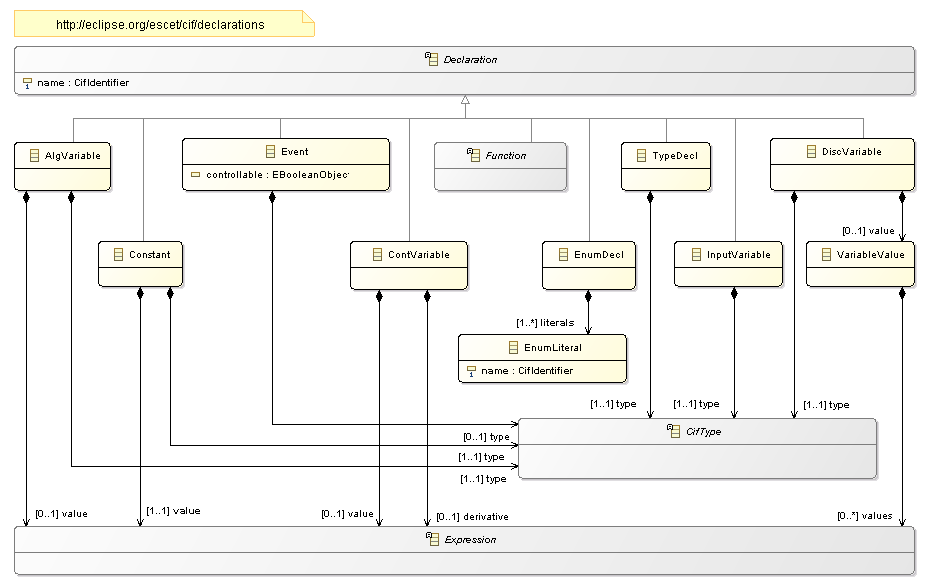
\includegraphics[width=\textwidth]{../model/images/declarations.png}
  \caption{\textit{declarations} package}\label{fig:pkg:declarations}
\end{figure}

Figure~\ref{fig:pkg:declarations} shows the \textit{declarations} package.
This package contains declaration classes used to declare `small' objects
(compared to for instance component definitions). The \cifclass{Declaration}
class is the main class. All declarations have a name. Note that the
\cifclass{Function} class is further defined in the \textit{functions}
package.
}

% AlgVariable (class)
\newcommand{\clsdocuAlgVariable}{
An algebraic variable declaration. An algebraic variable is a shortcut for an
expression. Everywhere the algebraic variable is used, its defining expression
could be used instead. Note that references to other objects in the expression
that defines the algebraic variable, are resolved in the context where the
algebraic variable is defined, and not in the context where the algebraic
variable is used.

A difference with constants is that constants must have constant values, while
algebraic variables may depend on the values of for instance variables and
locations. Another difference is in scoping. See also
Section~\ref{sec:scoping}.

Note that in the CIF textual syntax, the range of an integer type of an
algebraic variable, is optional. If it is not specified, and a range can be
determined for the value of the algebraic variable, that range is used as the
range of the type of the algebraic variable as well. This only applies to
algebraic variables that have an integer type directly. It for instance does
not apply to lists of integers.

\begin{constraints}
\citem{AlgVariable.typeValueMatch}
  The \emph{type} and \emph{value} (if specified) of the algebraic variable
  must match. This constraint does not apply to algebraic parameters. For
  integer types, the range of the type of the value must be entirely contained
  in the range of the type of the algebraic variable.
\end{constraints}
}

\newcommand{\featdocuAlgVariabletype}{
The type of the algebraic variable.

\begin{constraints}
\citem{AlgVariable.allowedTypes}
  Component and component definition types are not allowed for algebraic
  variables.
\end{constraints}
}

\newcommand{\featdocuAlgVariablevalue}{
The value of the algebraic variable (the defining expression).

\begin{constraints}
\citem{AlgVariable.selfReference}
  The value of an algebraic variable may not, directly or indirectly, refer to
  the algebraic variable itself. That is, an algebraic variable may not be
  defined in terms of itself. This includes the value of the algebraic
  variable (regardless of whether it is defined with the declaration or in
  one or more equations).
\citem{AlgVariable.uniqueValue}
  For each algebraic variable, the value must be uniquely defined. That
  is, either it is defined with the declaration itself (and not in any
  equation), or it is defined in a single equation in the same scope as where
  the variable is declared (and not in the declaration itself, not in multiple
  equations), or it is defined in an equation for each of the locations of the
  automaton that the variable is declared in (and not in the declaration
  itself, not in any equation in the automaton itself, not more than once per
  location).

  For algebraic variables that are part of an algebraic parameter, the value
  must not be set, since then the arguments should provide the value.
  See also the \cifclass{AlgParameter} class constraints.
\end{constraints}
}

% Constant (class)
\newcommand{\clsdocuConstant}{
A constant declaration. A constant is a shortcut for a constant value.
Everywhere the constant is used, its defining value could be used instead.
Note that references to other objects in the value expression that defines
the constant, are resolved in the context where the constant is defined, and
not in the context where the constant is used.

A difference with algebraic variables is that constants must have constant
values, while algebraic variable may depend on the values of for instance
variables and locations. Another difference is in scoping. See also
Section~\ref{sec:scoping}.

Note that in the CIF textual syntax, the range of an integer type of a constant,
is optional. If it is not specified, and a range can be determined for the
value of the constant, that range is used as the range of the type of the
constant as well. This only applies to constants that have an integer type
directly. It for instance does not apply to lists of integers.

\begin{constraints}
\citem{Constant.typeValueMatch}
  The \emph{type} and \emph{value} of the constant must match. For integer
  types, the range of the type of the value must be entirely contained in
  the range of the type of the constant.
\end{constraints}
}

\newcommand{\featdocuConstanttype}{
The type of the constant.

\begin{constraints}
\citem{Constant.allowedTypes}
  Component and component definition types are not allowed for constants.
\end{constraints}
}

\newcommand{\featdocuConstantvalue}{
The value of the constant (the defining expression).

\begin{constraints}
\citem{Constant.selfReference}
  The value of a constant may not, directly or indirectly, refer to the
  constant itself. That is, a constant may not be defined in terms of itself.
\citem{Constant.constantValue}
  The value of a constant must be constant, and may thus not refer to objects
  that can change value, such as discrete and algebraic variables. Note that
  expressions may refer to locations (`is the location active'). Since they can
  change as well, location references are not allowed either.

  Furthermore, user-defined functions are explicitly disallowed, as we can't
  statically determine whether they terminate.
\end{constraints}
}

% ContVariable (class)
\newcommand{\clsdocuContVariable}{
A continuous variable declaration. Continuous variables are implicitly real
typed variables, which change value according to their derivative, as time
passes.

Continuous variable declared in an \cifclass{Automaton}, may only be assigned
in the automaton in which they are declared. If they are not declared in an
automaton, they may not be assigned anywhere. They can however be accessed
(read) elsewhere.

\begin{constraints}
\citem{ContVariable.selfReference}
  The initial value of a continuous variable may not, directly or indirectly,
  refer to the continuous variable itself. That is, a continuous variable may
  not be defined in terms of itself. This includes the initial value of the
  continuous variable, but not its derivative (regardless of whether it is
  defined with the declaration or in one or more equations), which may be
  defined in terms of the continuous variable itself.

  The derivative of a continuous variable may not, directly or indirectly,
  refer to the derivative of that continuous variable itself. That is, a
  derivative may not be defined in terms of itself (regardless of whether it is
  defined with the declaration or in one or more equations).
\citem{ContVariable.uniqueDerivative}
  For each continuous variable, the derivative must be uniquely defined. That
  is, either it is defined with the declaration itself (and not in any
  equation), or it is defined in a single equation in the same scope as where
  the variable is declared (and not in the declaration itself, not in multiple
  equations), or it is defined in an equation for each of the locations of the
  automaton that the variable is declared in (and not in the declaration
  itself, not in any equation in the automaton itself, not more than once per
  location).
\end{constraints}
}

\newcommand{\featdocuContVariablederivative}{
The derivative of the continuous variable.

\begin{constraints}
\citem{ContVariable.derivativeType}
  If specified, the type of the derivative must be a real type.
\end{constraints}
}

\newcommand{\featdocuContVariablevalue}{
The initial value of the continuous variable. If not specified, defaults to
value \texttt{0.0}.

\begin{constraints}
\citem{ContVariable.valueType}
  If specified, the type of the initial value must be a real type.
\end{constraints}
}

% Declaration (abstract class)
\newcommand{\clsdocuDeclaration}{
Base class for `small' (compared to for instance component definitions)
CIF object declarations.
}

\newcommand{\featdocuDeclarationname}{
The name of the declaration.

\begin{constraints}
\citemnf{Declaration.name}
  Declaration names for non-event declarations must not start with
  \texttt{e\_}, \texttt{c\_}, or \texttt{u\_}, as those names are reserved
  for events.
\end{constraints}
}

% DiscVariable (class)
\newcommand{\clsdocuDiscVariable}{
A discrete variable declaration.

Discrete variables declared in automata are always local to the
\cifclass{Automaton} in which they are declared, and can be assigned
(modified) only in that automaton. They can however be accessed (read)
elsewhere.

This class is also used for the parameters and local variables of internal
user-defined functions.

\begin{constraints}
\citem{DiscVariable.typeValueMatch}
  Each of the possible values of the discrete variable, if specified, must
  match the type of the discrete variable. If the type of the discrete variable
  has a range, the ranges of the types of the values must be entirely contained
  in the range of the type of the discrete variable.
\citem{DiscVariable.occurrence}
  Discrete variables may not be declared in groups (including
  specifications). That is, they must be declared in automata.

  They may also be used in function parameters and as local variables in
  functions, but then they are usually not called discrete variables.
\end{constraints}
}

\newcommand{\featdocuDiscVariabletype}{
The type of the discrete variable.

\begin{constraints}
\citem{DiscVariable.allowedTypes}
  Component and component definition types are not allowed for discrete
  variables.
\end{constraints}
}

\newcommand{\featdocuDiscVariablevalue}{
The initial value of the discrete variable. If not specified, it has the
default value for its type. The default values for each type are:

\begin{itemize}
\item Booleans: \emph{false},
\item Integers (ranged): the value in the range that is closest to zero,
\item Integers (rangeless): \emph{0},
\item Reals: \emph{0.0},
\item Strings: \emph{""},
\item List (rangeless): empty list,
\item List (ranged): list with as few elements as possible, with each element
  the default value of the element type,
\item Set: empty set,
\item Dictionary: empty dictionary,
\item Tuple: tuple with for each field, the default value for the type of the
  field,
\item Function: function that returns the default value for the return type
  of the function,
\item Distribution: constant distribution with value \emph{false} for boolean
  distributions, \emph{0} for integer distributions, and \emph{0.0} for real
  distributions,
\item Enumerations: the first enumeration literal defined in the enumeration.
\end{itemize}

Some examples of default values for different integer ranges:

\begin{tabular}{ll}
\textbf{Range} & \textbf{Default value} \\
\hline
\range{0}{5}   & $0$  \\
\range{2}{5}   & $2$  \\
\range{-5}{-2} & $-2$ \\
\range{-5}{5}  & $0$  \\
\range{-5}{0}  & $0$  \\
\hline
\end{tabular}

Some examples of default values for different list types:

\begin{tabular}{ll}
\textbf{List type}       & \textbf{Default value} \\
\hline
\texttt{list int}        & \emph{[]}         \\
\texttt{list[3] int}     & \emph{[0, 0, 0]}  \\
\texttt{list[2..5] real} & \emph{[0.0, 0.0]} \\
\hline
\end{tabular}

\begin{constraints}
\citem{DiscVariable.selfReference}
  The values of a discrete variable may not, directly or indirectly, refer to
  the discrete variable itself. That is, a discrete variable may not be
  defined in terms of itself.
\end{constraints}
}

% EnumDecl (class)
\newcommand{\clsdocuEnumDecl}{
An enumeration declaration. An enumeration is a strongly typed set of values,
and is often clearer than arbitrary numbers.

Note that for equality purposes, two enumerations that define the same sequence
of values (same number of values, with the same names, in the same order), are
considered compatible types, and their enumeration literals (the values) can be
compared for equality.

Note that for scoping purposes, the literals are defined at the same level as
the enumeration declaration itself. This ensures that in the CIF textual syntax,
we don't have to prefix enumeration literals with the name of the enumeration
declaration.

\begin{constraints}
\citem{EnumDecl.uniqueLiterals}
  The names of the enumeration literals of the enumeration declarations must
  be unique with respect to the other literals defined in that same
  enumeration, as well as all the declarations at the same level as the
  enumeration declaration that the literals are a part of.
\end{constraints}
}

\newcommand{\featdocuEnumDeclliterals}{
The enumeration literals (values) that make up this enumeration.
}

% EnumLiteral (class)
\newcommand{\clsdocuEnumLiteral}{
An enumeration literal (value) as part of an \cifclass{EnumDecl}.
}

\newcommand{\featdocuEnumLiteralname}{
The name of the enumeration literal.

\begin{constraints}
\citemnf{EnumLiteral.name}
  Enumeration literal names must not start with \texttt{e\_}, \texttt{c\_}, or
  \texttt{u\_}, as those prefixes are reserved for events.
\end{constraints}
}

% Event (class)
\newcommand{\clsdocuEvent}{
An event declaration.

Note that events that are not in the alphabet of any automaton, are globally
disabled, since the alphabet of the specification is the union of the alphabets
of the automata. In other words, if an event is not used on any edge, it is
globally disabled. Event `tau' is an exception, as it is never in the alphabet,
since `tau' does not synchronize. Channels are exceptions as well, as they
require exactly one sender and one receiver, and if not further restricted by
any synchronizing automata, they are pure channels.

\begin{constraints}
\citemnf{Event.matchNameControllability}
  If the name of the event starts with \texttt{c\_}, the event must be defined
  to be controllable. If the name of the event starts with \texttt{u\_}, the
  event must be defined to be uncontrollable. If the name of the event starts
  with \texttt{e\_}, the event must not be defined to be controllable or
  uncontrollable. This is to ensure that the naming convention (which is also
  used for syntax highlighting), is not violated.
\end{constraints}
}

\newcommand{\featdocuEventcontrollable}{
Indicates the controllability of the event. If \emph{true}, the event is
controllable. If \emph{false}, the event is uncontrollable. If \emph{null},
the event is not defined as controllable or uncontrollable.
}

\newcommand{\featdocuEventtype}{
The type of the data communicated via this event, if applicable.

\begin{constraints}
\citem{Event.allowedTypes}
  Component and component definition types are not allowed for events.
\end{constraints}
}

% InputVariable (class)
\newcommand{\clsdocuInputVariable}{
An input variable declaration. An input variable is a variable for which the
value is not defined by the CIF specification, but by an external source.
It is allowed for the values of input variables to change at any time
(discontinuously), depending on the external source. Input variables are
read-only in the CIF specification.
}

\newcommand{\featdocuInputVariabletype}{
The type of the input variable.

\begin{constraints}
\citem{InputVariable.allowedTypes}
  Component and component definition types are not allowed for input variables.
\end{constraints}
}

% TypeDecl (class)
\newcommand{\clsdocuTypeDecl}{
A type declaration. Defines a reusable type. Mostly useful for types that
have somewhat larger textual forms, which can then be referred to by name.
}

\newcommand{\featdocuTypeDecltype}{
The type of the type declaration. This type and the type declaration have
compatible (equal) types.

\begin{constraints}
\citem{TypeDecl.allowedTypes}
  Component and component definition types are not allowed.
\citem{TypeDecl.selfReference}
  The type of a type declaration may not, directly or indirectly, refer to the
  type declaration itself. That is, a type declaration may not be defined in
  terms of itself.
\end{constraints}
}

% VariableValue (class)
\newcommand{\clsdocuVariableValue}{
Set of values that represents possible initial values of a
\cifclass{DiscVariable}.
}

\newcommand{\featdocuVariableValuevalues}{
The possible initial values of the variable. If one or more values are
specified, the initial value of the variable is one of those values. If no
value is given, the variable can have any value in its domain.
}


%%%%%%%%%%%%%%%%%%%%%%%%%%%%%%%%%%%%%%%%%%%%%%%%%%%%%%%%%%%%%%%%%%%%%%%%%%%%%%%
% Package automata
%%%%%%%%%%%%%%%%%%%%%%%%%%%%%%%%%%%%%%%%%%%%%%%%%%%%%%%%%%%%%%%%%%%%%%%%%%%%%%%
\newcommand{\pkgdocuautomata}{
\begin{figure}
  \centering
  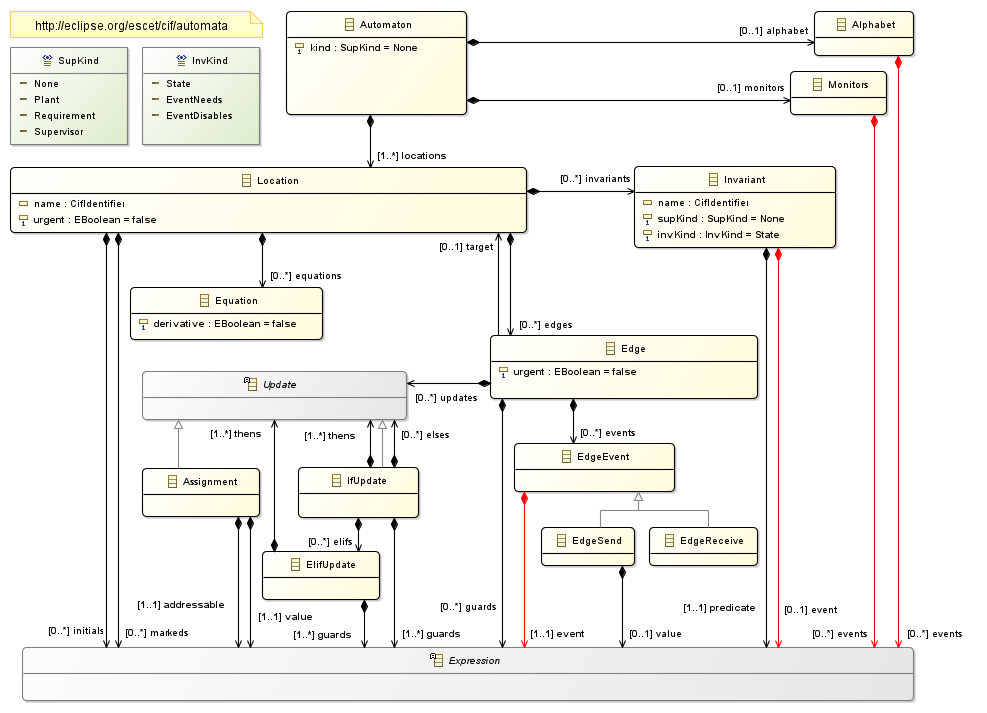
\includegraphics[width=\textwidth]{../model/images/automata.png}
  \caption{\textit{automata} package}\label{fig:pkg:automata}
\end{figure}

Figure~\ref{fig:pkg:automata} shows the \textit{automata} package.
This package contains classes related to automata. The \cifclass{Automaton}
class is the main class. Automata have at least one location. They may
optionally also have an alphabet. Locations may have outgoing edges, and edges
may have guards, updates, and events. This corresponds to most other
automaton-based languages.
}

% Alphabet (class)
\newcommand{\clsdocuAlphabet}{
An alphabet of an \cifclass{Automaton}.
}

\newcommand{\featdocuAlphabetevents}{
The events that define the alphabet. May be empty to denote an empty alphabet.
It is not possible to include the `tau' event in alphabets.

This feature contains \cifclass{Expression} instances, to allow for wrapping
expressions to be used. See also Section~\ref{sec:scoping}.

\begin{constraints}
\citemnf{Alphabet.uniqueEvents}
  Alphabets must contain unique events.
\citem{Alphabet.eventRefsOnly}
  The expressions must refer to events.
\citem{Alphabet.eventsInScope}
  The event references must satisfy the scoping rules.
\citem{Alphabet.eventParamSync}
  If an event reference refers to an event parameter, the event parameter
  should allow synchronization use. That is, the event parameter should not
  specify any flags (allow all usages) or should explicitly specify the
  synchronization ($\sim$) flag to allow synchronization.
\end{constraints}
}

% Assignment (class)
\newcommand{\clsdocuAssignment}{
An assignment update.

\begin{constraints}
\citem{Assignment.types}
  The type of the assigned value must match the type of the addressable that is
  assigned. If the variable being assigned has a ranged type, then the range of
  the type of the value must have overlap with the range of the type of the
  variable. It is considered a run-time error if the evaluated value expression
  results in a value that is outside of the range of the assigned variable.
\end{constraints}
}

\newcommand{\featdocuAssignmentaddressable}{
The addressable (a variable, a part of a variable, multiple variables, parts
of multiple variables, etc) to which to assign a value.

It is allowed to create a new key/value pair in a dictionary, if the key of the
last projection does not exist. It is not allowed to create a new key/value
pair, if the key of one of the other projections does not exist.

The indices of the projections of the addressables are evaluated in the
`old' state.

\begin{constraints}
\citem{Assignment.addressableSyntax}
  Addressables on edges may be discrete and continuous variable references 
  (possibly wrapped) with projections, and addressables in CIF/SVG input mappings may
  be input variable references (possibly wrapped) with projections. The variable
  references may optionally be wrapped in tuples (possibly multiple times). Projected
  string typed variables are not allowed.
\citem{Assignment.variablesInScope}
  The variables that are assigned on edges must be discrete or continuous
  variables declared in the automaton that contains the source location of the
  edge of this assignment update. Discrete and continuous variables may be mixed
  in a single assignment. The variables that are assigned in CIF/SVG input mappings
  must be input variables.
\end{constraints}
}

\newcommand{\featdocuAssignmentvalue}{
The value to assign to the variable(s).

This expression is evaluated in the `old' state.
}

% Automaton (class)
\newcommand{\clsdocuAutomaton}{
An automaton component. This class is the basic leaf component of all component
hierarchies.

All invariants at this level are combined using logical
conjunction operators. The location invariants are combined
with the location itself, using logical implication operators. Assuming
we have local invariants $i_1, i_2, \ldots, i_n$, and we have
locations $l_1, l_2, \ldots, l_m$, with location invariants
$j_1, j_2, \ldots, j_m$, then the invariant for the entire
automaton becomes:
\[\bigwedge_{a=1}^n i_a \land \bigwedge_{b=1}^m l_b \Rightarrow j_b\]

In a similar way, the local initialization predicates are combined with the
location initialization predicates, and the local marker predicates are
combined with the location marker predicates.

Note that this uses mathematical conjunctions, and not the short-circuit
conjunction binary operators. As such, there is no ordering between invariants,
between initialization predicates, and between marker predicates.

\begin{constraints}
\citem{Automaton.uniqueDecls}
  The names of all declarations, invariants and locations defined in an
  automaton must be unique within that automaton.
\citem{Automaton.validAlphabet}
  If an alphabet is specified, it must contain at least the events that occur
  on the edges of this automaton (excluding communication usage by means of
  sends and receives). Note that the `tau' event is never part of alphabets.
\citem{Automaton.noFuncDecl}
  Functions may not be defined in automata.
\citem{Automaton.uniqueUsagePerEvent}
  Each automaton must use a certain event in at most one way: synchronization,
  sending, or receiving. The events that are used to synchronize are determined
  by the alphabet. The send/receive uses are found via the edges.
\end{constraints}
}

\newcommand{\featdocuAutomatonalphabet}{
The alphabet of the automaton. If not specified, it defaults to the events used
on the edges of the automaton (excluding communication usage by means of sends
and receives). Note that the `tau' event is never part of alphabets.
}

\newcommand{\featdocuAutomatonkind}{
The supervisory kind of the automaton.
}

\newcommand{\featdocuAutomatonlocations}{
The locations of the automaton.
}

\newcommand{\featdocuAutomatonmonitors}{
The monitor events of the automaton. For details on monitors, see the
\cifclass{Monitors} class.

If not specified, the automaton does not monitor any events.
}

% Edge (class)
\newcommand{\clsdocuEdge}{
An outgoing edge of a \cifclass{Location} of an \cifclass{Automaton}.
}

\newcommand{\featdocuEdgeevents}{
The events of the edge. Specifying multiple events is equivalent to duplicating
the edge, with each edge containing one of the events of the original edge.
Specifying no events is equivalent to specifying a single `tau' event.

This feature contains \cifclass{Expression} instances, to allow for wrapping
expressions to be used. See also Section~\ref{sec:scoping}.

\begin{constraints}
\citemnf{Edge.uniqueEvents}
  Edges must contain unique events.
\citem{Edge.oneReceiveAllReceive}
  If one of the events performs a receive, the other events on that same edge
  must also perform receives, and the data types of their events must be equal.
  This is to ensure that the received value reference expression (if used), is
  available, and has a consistent type.

  We don't allow unequal but compatible types, as that would lead to a union
  of those types for the received value reference expression, and that would
  lead to a difference in type for multiple events on a single edge, and
  multiple edges with one event each.
\end{constraints}
}

\newcommand{\featdocuEdgeguards}{
The guard predicates of the edge. An edge is only enabled if the guard
evaluates to true in the current state.

If no predicates are given, the guard predicate is \emph{true}. If
multiple predicates are given, this feature represents the logical conjunction
of those predicates. Note that this represents the mathematical conjunction,
and not the short-circuit conjunction binary operator. As such, there is
no ordering between the guards of an edge.

\begin{constraints}
\citem{Edge.guardTypes}
  The guard predicates must have boolean types.
\end{constraints}
}

\newcommand{\featdocuEdgetarget}{
The target location (within this automaton) of the edge. If not set, the
edge is a self-loop, which means that the target location of the edge is equal
to the source location of the edge.

\begin{constraints}
\citem{Edge.targetInScope}
  The target location of the edge, if specified, must be declared in the same
  automaton as the source location of the edge. In particular, location
  parameters of component definitions are not allowed.
\end{constraints}
}

\newcommand{\featdocuEdgeupdates}{
The updates to execute if the edge is `executed'.

\begin{constraints}
\citem{Edge.uniqueVariables}
  The parts of the variables that are assigned must be unique. That is, it must
  never be possible to assign the same part of the same variable twice.

  Since we don't include the guards of conditional updates in the analysis,
  this may lead to false positives. We believe that in such cases, the update
  can easily be rewritten, and thus the false positives will not be a problem
  in practice.

  We include the projections in the analysis. For tuple projections, the index
  can always be statically evaluated, as the type checker needs the index to
  get the type of the field. Tuple field references are normalized to 0-based
  field indices. For lists, indices are evaluated if this is possible
  statically. Negative array indices are normalized. For non-array lists,
  negative indices can not be normalized statically. For dictionaries, the keys
  are statically evaluated, if possible. Since not all expressions can be
  statically evaluated, and also normalization is not always possible
  statically, overlap of parts of variables can not always be properly
  detected, potentially leading to false positives. We opt for false positives
  rather than runtime checks, to avoid having to handle such cases in many
  tools and transformations.
\end{constraints}
}

\newcommand{\featdocuEdgeurgent}{
Whether the edge is urgent. If an edge is urgent, and the guard is enabled,
then time may not progress.

\begin{constraints}
\citemnf{Edge.urgWhenLocUrg}
  An edge should not be urgent when the source location of the edge is also
  urgent, as that adds no additional constraint or behavior.
\end{constraints}
}

% EdgeEvent (class)
\newcommand{\clsdocuEdgeEvent}{
An event of an edge. Optionally with communication, see derived classes.
}

\newcommand{\featdocuEdgeEventevent}{
The event reference of the edge event.

This feature contains an \cifclass{Expression} instance, to allow for wrapping
expressions to be used. See also Section~\ref{sec:scoping}.

\begin{constraints}
\citem{EdgeEvent.eventRefsOnly}
  The expression must refer to an event.
\citem{EdgeEvent.eventsInScope}
  The event references must satisfy the scoping rules.
\citem{EdgeEvent.eventParamUse}
  If an event reference refers to an event parameter, the event parameter
  should allow the use of the event as it is used on this edge. That is, the
  event parameter should not specify any flags (allow all usages) or should
  explicitly specify the flag that allows the usage on this edge.
\end{constraints}
}

% EdgeReceive (class)
\newcommand{\clsdocuEdgeReceive}{
A receive event of an edge.

\begin{constraints}
\citem{EdgeReceive.commEvent}
  The \emph{event} must have a data type.
\end{constraints}
}

% EdgeSend (class)
\newcommand{\clsdocuEdgeSend}{
A send event of an edge.

\begin{constraints}
\citem{EdgeSend.commEvent}
  The \emph{event} must have a data type.
\end{constraints}
}

\newcommand{\featdocuEdgeSendvalue}{
The value to send as part of the communication. This expression is evaluated
in the `old' state, before any updates are processed.

\begin{constraints}
\citem{EdgeSend.allowedValue}
  If the \emph{event} has a non-void data type, then the \emph{value} is
  required. If the data type is \cifclass{VoidType}, then a \emph{value} is
  not allowed.
\citem{EdgeEvent.valueType}
  The type of the value must match the type of the event (first contained in
  the second).
\end{constraints}
}

% ElifUpdate (class)
\newcommand{\clsdocuElifUpdate}{
An `elif' (`else-if') alternative of an \cifclass{IfUpdate}.
}

\newcommand{\featdocuElifUpdateguards}{
The guard predicates for this alternative.

If multiple predicates are given, this feature represents the logical
conjunction of those predicates. Note that this represents the mathematical
conjunction, and not the short-circuit conjunction binary operator. As such,
there is no ordering between the guards.

\begin{constraints}
\citem{ElifUpdate.guardTypes}
  The guard predicates must have boolean types.
\end{constraints}
}

\newcommand{\featdocuElifUpdatethens}{
The update to execute for the \cifclass{ElifUpdate} if the `guards'
evaluate to \emph{true}.
}

% IfUpdate (class)
\newcommand{\clsdocuIfUpdate}{
A conditional update.
}

\newcommand{\featdocuIfUpdateelifs}{
The `else-if' (`elif') alternatives. Processed in order, if the `guards'
evaluate to \emph{false}.
}

\newcommand{\featdocuIfUpdateelses}{
The `else' updates. Executed if no other alternative has a \emph{true} guard.
}

\newcommand{\featdocuIfUpdateguards}{
The guard predicates for the `then' updates.

If multiple predicates are given, this feature represents the logical
conjunction of those predicates. Note that this represents the mathematical
conjunction, and not the short-circuit conjunction binary operator. As such,
there is no ordering between the guards.

\begin{constraints}
\citem{IfUpdate.guardTypes}
  The guard predicates must have boolean types.
\end{constraints}
}

\newcommand{\featdocuIfUpdatethens}{
The `then' updates. Executed if the `guards' evaluate to \emph{true}.
}

% Location (class)
\newcommand{\clsdocuLocation}{
A location of an \cifclass{Automaton}.
}

\newcommand{\featdocuLocationedges}{
The outgoing edges of the location.
}

\newcommand{\featdocuLocationequations}{
The equations of the location.
}

\newcommand{\featdocuLocationinitials}{
The initialization predicates of the location. A CIF model can only start in
states that satisfy the initialization predicates.

If no predicates are given, the initialization predicate is \emph{false}. If
multiple predicates are given, this feature represents the logical conjunction
of those predicates. Note that this represents the mathematical conjunction,
and not the short-circuit conjunction binary operator. As such, there is
no ordering between initialization predicates.

\begin{constraints}
\citem{Location.initialTypes}
  The initialization predicates must have boolean types.
\end{constraints}
}

\newcommand{\featdocuLocationinvariants}{
The invariants of the location. A CIF model can only be in a state
if that state satisfies the invariants.

If no invariants are given, the invariant is \emph{true}. If multiple
invariants are given, this feature represents the logical conjunction
of those invariants. Note that this represents the mathematical conjunction,
and not the short-circuit conjunction binary operator. As such, there is
no ordering between invariants.
}

\newcommand{\featdocuLocationmarkeds}{
The marker predicates of the location. Used as liveness property for,
among others, supervisory controller synthesis.

If no predicates are given, the marker predicate is \emph{false}. If
multiple predicates are given, this feature represents the logical conjunction
of those predicates. Note that this represents the mathematical conjunction,
and not the short-circuit conjunction binary operator. As such, there is
no ordering between marker predicates.

\begin{constraints}
\citem{Location.markedTypes}
  The marker predicates must have boolean types.
\end{constraints}
}

\newcommand{\featdocuLocationname}{
The name of the location. If a location is the only location in an automaton,
the name may be omitted, but then the location may not be referenced.

\begin{constraints}
\citem{Location.nameless}
  The name of a location must be set if one of the following conditions holds:
  (1) the location is not the only location of the automaton; (2) the location
  is referenced; (3) the location is a location parameter. In other words,
  if it is not a location parameter, it is the only location of the automaton,
  and it is never referenced, the name may be omitted.

  As for (2), it is not possible to refer to a nameless location in the CIF
  textual syntax. However, it is possible to do that in the metamodel, and as
  such the situation can result from for instance a model transformation.
\citemnf{Location.name}
  Location names must not start with \texttt{e\_}, \texttt{c\_}, or
  \texttt{u\_}, as those prefixes are reserved for events.
\end{constraints}
}

\newcommand{\featdocuLocationurgent}{
Whether the location is urgent. If a location is urgent, then time may not
progress in that location.
}

% Monitors (class)
\newcommand{\clsdocuMonitors}{
The monitor events of an \cifclass{Automaton}.

Automata that monitor events are used to monitor (track, observe) the
behavior (or progress) of those monitor events, as initiated by other
components. Monitoring is often used for verification components, supervisors,
etc.

Informally, if an automaton monitors an event, the event is never blocked by
that automaton (guard-wise).
}

\newcommand{\featdocuMonitorsevents}{
The set of monitor events.

If no events are specified for this feature, the automaton monitors all events
in its alphabet. This differs from an automaton not having a
\cifclass{Monitors} instance at all, as that means the automaton does not
monitor any events at all.

This feature contains \cifclass{Expression} instances, to allow for wrapping
expressions to be used. See also Section~\ref{sec:scoping}.

\begin{constraints}
\citemnf{Automaton.monitorsUniqueEvents}
  The set of monitor events must contain unique events.
\citem{Automaton.monitorsEventRefsOnly}
  The expressions must refer to events. Event `tau' is not allowed, as that
  event is never part of the alphabet, as it does not synchronize with other
  automata.
\citem{Automaton.monitorsEventsInScope}
  The event references must satisfy the scoping rules.
\citem{Automaton.monitorsSubsetAlphabet}
  The set of monitor events must be a subset of the alphabet.
\end{constraints}
}

% Update (abstract class)
\newcommand{\clsdocuUpdate}{
An update of an \cifclass{Edge} or \cifclass{SvgIn}.
}


%%%%%%%%%%%%%%%%%%%%%%%%%%%%%%%%%%%%%%%%%%%%%%%%%%%%%%%%%%%%%%%%%%%%%%%%%%%%%%%
% Package types
%%%%%%%%%%%%%%%%%%%%%%%%%%%%%%%%%%%%%%%%%%%%%%%%%%%%%%%%%%%%%%%%%%%%%%%%%%%%%%%
\newcommand{\pkgdocutypes}{
\begin{figure}
  \centering
  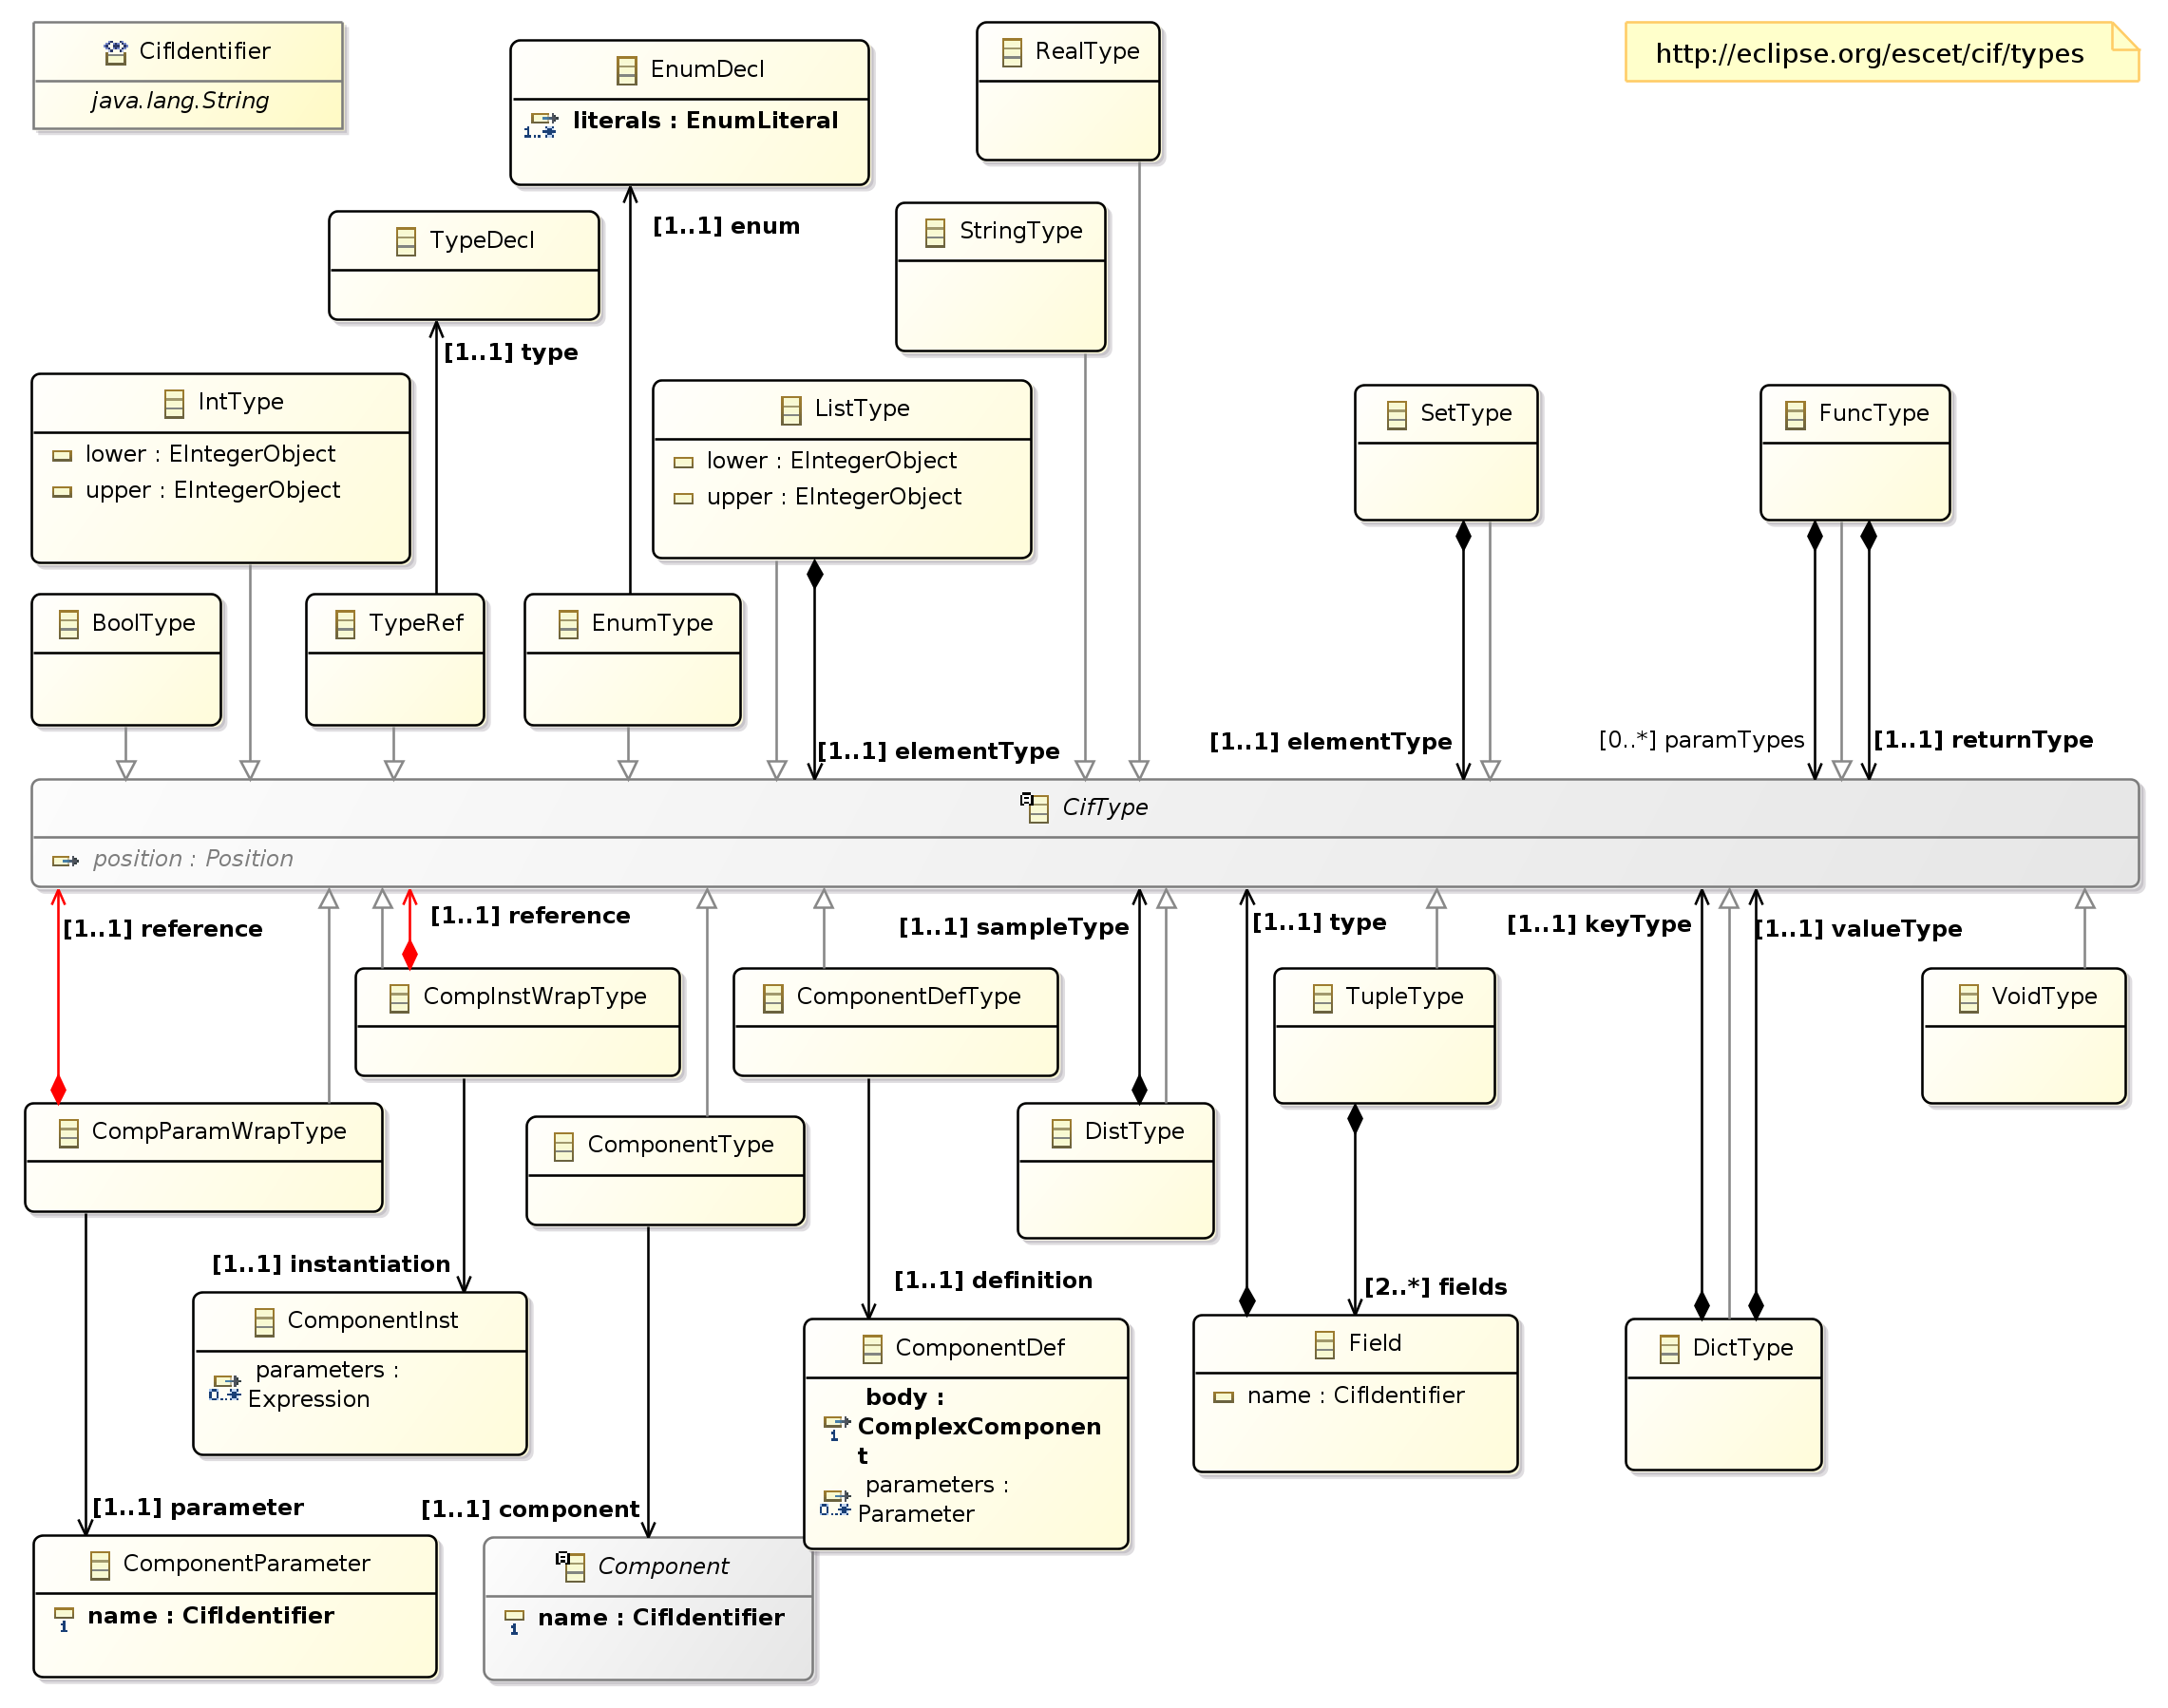
\includegraphics[width=\textwidth]{../model/images/types.png}
  \caption{\textit{types} package}\label{fig:pkg:types}
\end{figure}

Figure~\ref{fig:pkg:types} shows the \textit{types} package.
This package contains type classes, and is pretty standard compared to
other languages. The \cifclass{CifType} class is the main class. Of
particular interest may be the \cifclass{CompParamWrapType} and
\cifclass{CompInstWrapType} classes. They are used to keep track of references
via component parameters and component instantiations. See also
Section~\ref{sec:scoping}.
}

% BoolType (class)
\newcommand{\clsdocuBoolType}{
A boolean type. Represents boolean values.
}

% CifType (abstract class)
\newcommand{\clsdocuCifType}{
Base class for all CIF types.
}

% CompInstWrapType (class)
\newcommand{\clsdocuCompInstWrapType}{
Component instantiation reference wrapping type. Allows keeping track
of references via component instantiations. Similar to the
\cifclass{CompInstWrapExpression} class, but for type references instead of
expression references. Similar to the \cifclass{CompParamWrapType} class,
but for references via component instantiations instead of via component
parameters. See also Section~\ref{sec:scoping}.
}

\newcommand{\featdocuCompInstWrapTypeinstantiation}{
The component instantiation via which the object is referenced.

\begin{constraints}
\citem{CompInstWrapType.noCompDefBody}
  Components instantiations that are bodies of component definitions may not
  be referenced here, as the body \emph{is} the component definition.
\citem{CompInstWrapType.instantiationInScope}
  The component instantiation reference must satisfy the scoping rules.
\end{constraints}
}

\newcommand{\featdocuCompInstWrapTypereference}{
The object that is referenced via a component instantiation.

This feature contains \cifclass{CifType} instances, to allow for wrapping
types to be used.

\begin{constraints}
\citem{CompInstWrapType.reference}
  The \emph{reference} type must be a reference.
\end{constraints}
}

% CompParamWrapType (class)
\newcommand{\clsdocuCompParamWrapType}{
Component parameter reference wrapping type. Allows keeping track
of references via component parameters. Similar to the
\cifclass{CompParamWrapExpression} class, but for type references instead of
expression references. Similar to the \cifclass{CompInstWrapType} class,
but for references via component parameters instead of via component
instantiations. See also Section~\ref{sec:scoping}.
}

\newcommand{\featdocuCompParamWrapTypeparameter}{
The component parameter via which the object is referenced.

\begin{constraints}
\citem{CompParamWrapType.parameterInScope}
  The component parameter reference must satisfy the scoping rules.
\end{constraints}
}

\newcommand{\featdocuCompParamWrapTypereference}{
The object that is referenced via a component parameter.

This feature contains \cifclass{CifType} instances, to allow for wrapping
types to be used.

\begin{constraints}
\citem{CompParamWrapType.reference}
  The \emph{reference} type must be a reference.
\end{constraints}
}

% ComponentDefType (class)
\newcommand{\clsdocuComponentDefType}{
A component definition type.
}

\newcommand{\featdocuComponentDefTypedefinition}{
The component definition that is used as a type.

\begin{constraints}
\citem{ComponentDefType.definitionInScope}
  The component definition reference must satisfy the scoping rules.
\end{constraints}
}

% ComponentType (class)
\newcommand{\clsdocuComponentType}{
A component type.
}

\newcommand{\featdocuComponentTypecomponent}{
The component that is used as a type.

\begin{constraints}
\citem{ComponentType.noCompDefBody}
  Components that are bodies of component definitions may not be referenced
  here, as the body \emph{is} the component definition. In such cases a
  \cifclass{ComponentDefType} should be used instead.
\citem{ComponentType.noSpec}
  Specifications, which are technically components, may not be referenced here,
  as they serve as outer grouping only. Note that in the CIF textual syntax,
  they can't be referenced either, as they don't have a name.
\citem{ComponentType.componentInScope}
  The component reference must satisfy the scoping rules.
\end{constraints}
}

% DictType (class)
\newcommand{\clsdocuDictType}{
A dictionary type. Represents collections of key/value pairs, where keys are
unique within a single dictionary.
}

\newcommand{\featdocuDictTypekeyType}{
The type of the keys of the dictionary.

\begin{constraints}
\citem{DictType.allowedKeyTypes}
  Component and component definition types, as well as function and
  distribution types, are not allowed for dictionary keys.
\end{constraints}
}

\newcommand{\featdocuDictTypevalueType}{
The type of the values of the dictionary.

\begin{constraints}
\citem{DictType.allowedValueTypes}
  Component and component definition types are not allowed for dictionary
  values.
\end{constraints}
}

% DistType (class)
\newcommand{\clsdocuDistType}{
A distribution type. Represents stochastic distributions that produce values
(samples) according to a certain probability function.
}

\newcommand{\featdocuDistTypesampleType}{
The type of the samples produces by the distribution.

\begin{constraints}
\citem{DistType.allowedSampleTypes}
  Only booleans, integers (without range), and reals are allowed as sample
  types.
\end{constraints}
}

% EnumType (class)
\newcommand{\clsdocuEnumType}{
An enumeration type. Represents the enumeration literals of a certain
enumeration.
}

\newcommand{\featdocuEnumTypeenum}{
The enumeration of which the enumeration literals make up this type.

\begin{constraints}
\citem{EnumRef.enumInScope}
  The enumeration reference must satisfy the scoping rules.
\end{constraints}
}

% Field (class)
\newcommand{\clsdocuField}{
A field of a tuple type.
}

\newcommand{\featdocuFieldname}{
The name of the field. Note that the name is mandatory in the CIF textual
syntax, but is optional to allow for anonymous tuple fields that result from
standard library functions, etc.
}

\newcommand{\featdocuFieldtype}{
The type of the field.

\begin{constraints}
\citem{Field.allowedTypes}
  Component and component definition types are not allowed for tuple fields.
\end{constraints}
}

% FuncType (class)
\newcommand{\clsdocuFuncType}{
A function type. Represents functions.
}

\newcommand{\featdocuFuncTypeparamTypes}{
The types of the parameters of the function.

\begin{constraints}
\citem{FuncType.allowedParamTypes}
  Component and component definition types are not allowed for function
  parameters.
\end{constraints}
}

\newcommand{\featdocuFuncTypereturnType}{
The type of the result of the function.

\begin{constraints}
\citem{FuncType.allowedReturnTypes}
  Component and component definition types are not allowed for function
  return values.
\end{constraints}
}

% IntType (class)
\newcommand{\clsdocuIntType}{
An integer type. Represents a subset of all integer values.

The range of integer types is optional. If not specified, the range is
\range{-2^{31}}{2^{31}-1}. See also the \cifclass{IntExpression} class.

\begin{constraints}
\citem{IntType.neitherOrBoth}
  Either the \emph{lower} bound and the \emph{upper} bound are specified, or
  neither of them are.
\citem{IntType.validRange}
  If the bounds are specified, the \emph{lower} bound value must be less than
  or equal to the \emph{upper} bound value, to make sure we have a valid
  (non-empty) range.
\end{constraints}
}

\newcommand{\featdocuIntTypelower}{
The lower bound (inclusive) of the values that make up this type. If it is not
specified, it is implicitly $-2^{31}$.
}

\newcommand{\featdocuIntTypeupper}{
The upper bound (inclusive) of the values that make up this type. If it is not
specified, it is implicitly $2^{31}-1$.
}

% ListType (class)
\newcommand{\clsdocuListType}{
A list type. Represents ordered collections of elements, possibly with
duplicates.

The range of list types is optional. If not specified, the range is
\range{0}{2^{31}-1}. This follows from the use of integers for the ranges. See
also the \cifclass{IntType} and \cifclass{IntExpression} classes.

\begin{constraints}
\citem{ListType.neitherOrBoth}
  Either the \emph{lower} bound and the \emph{upper} bound are specified, or
  neither of them are.
\citem{ListType.nonNegativeRangeBounds}
  If the bounds are specified, they must be non-negative.
\citem{ListType.validRange}
  If the bounds are specified, the \emph{lower} bound value must be less than
  or equal to the \emph{upper} bound value, to make sure we have a valid
  (non-empty) range.
\end{constraints}
}

\newcommand{\featdocuListTypeelementType}{
The type of the elements of the list.

\begin{constraints}
\citem{ListType.allowedTypes}
  Component and component definition types are not allowed for list elements.
\end{constraints}
}

\newcommand{\featdocuListTypelower}{
The lower bound (inclusive) of the allowed sizes of the lists that are values
of this type. If it is not specified, it is implicitly $0$.
}

\newcommand{\featdocuListTypeupper}{
The upper bound (inclusive) of the allowed sizes of the lists that are values
of this type. If it is not specified, it is implicitly $2^{31}-1$.
}

% RealType (class)
\newcommand{\clsdocuRealType}{
A real type. Represents a subset of all real values.

Real values are implemented using Java's \texttt{double} data type, which is
conceptually associated with double-precision 64-bit format IEEE 754 values
as specified in IEEE Standard for Binary Floating-Point Arithmetic, ANSI/IEEE
Standard 754-1985 (IEEE, New York). The IEEE 754 standard includes not only
positive and negative numbers that consist of a sign and magnitude, but also
positive and negative zeros, positive and negative infinities, and a special
Not-a-Number (NaN) value. A NaN value is used to represent the result of
certain invalid operations such as dividing zero by zero. We explicitly
exclude positive and negative infinities, as wel as NaN values, and any
operation that results in them is considered a run-time evaluation error.
Negative zero values are automatically converted to positive zero values.
See also the \cifclass{RealExpression} class.
}

% SetType (class)
\newcommand{\clsdocuSetType}{
A set type. Represents unordered collections of elements, without duplicates.
}

\newcommand{\featdocuSetTypeelementType}{
The type of the elements of the set.

\begin{constraints}
\citem{SetType.allowedTypes}
  Component and component definition types, as well as function and
  distribution types, are not allowed for set elements.
\end{constraints}
}

% StringType (class)
\newcommand{\clsdocuStringType}{
A string type. Represents string values, in other words, it represents texts.
}

% TupleType (class)
\newcommand{\clsdocuTupleType}{
A tuple type. Represents ordered collections of elements, where the number of
elements is fixed, and each element can have a different type.
}

\newcommand{\featdocuTupleTypefields}{
The fields of the tuple.

\begin{constraints}
\citem{TupleType.uniqueFieldNames}
  The names of the fields of the tuple type must be unique with respect to
  the other fields defined in that same tuple type.
\end{constraints}
}

% TypeRef (class)
\newcommand{\clsdocuTypeRef}{
A type reference. Represents the same values as the values of the referred
type declaration.
}

\newcommand{\featdocuTypeReftype}{
The \cifclass{TypeDecl} that this type reference refers to.

\begin{constraints}
\citem{TypeRef.typeInScope}
  The type declaration reference must satisfy the scoping rules.
\end{constraints}
}

% VoidType (class)
\newcommand{\clsdocuVoidType}{
A void type. Used to represent the type of a channel over which no data is
communicated.

\begin{constraints}
\citem{VoidType.occurrence}
  The `void' type may only be used as type of events (and event parameters). It
  may not be used in other types (such as list types), in type declarations,
  etc.
\end{constraints}
}


%%%%%%%%%%%%%%%%%%%%%%%%%%%%%%%%%%%%%%%%%%%%%%%%%%%%%%%%%%%%%%%%%%%%%%%%%%%%%%%
% Package expressions
%%%%%%%%%%%%%%%%%%%%%%%%%%%%%%%%%%%%%%%%%%%%%%%%%%%%%%%%%%%%%%%%%%%%%%%%%%%%%%%
\newcommand{\pkgdocuexpressions}{
\begin{figure}
  \centering
  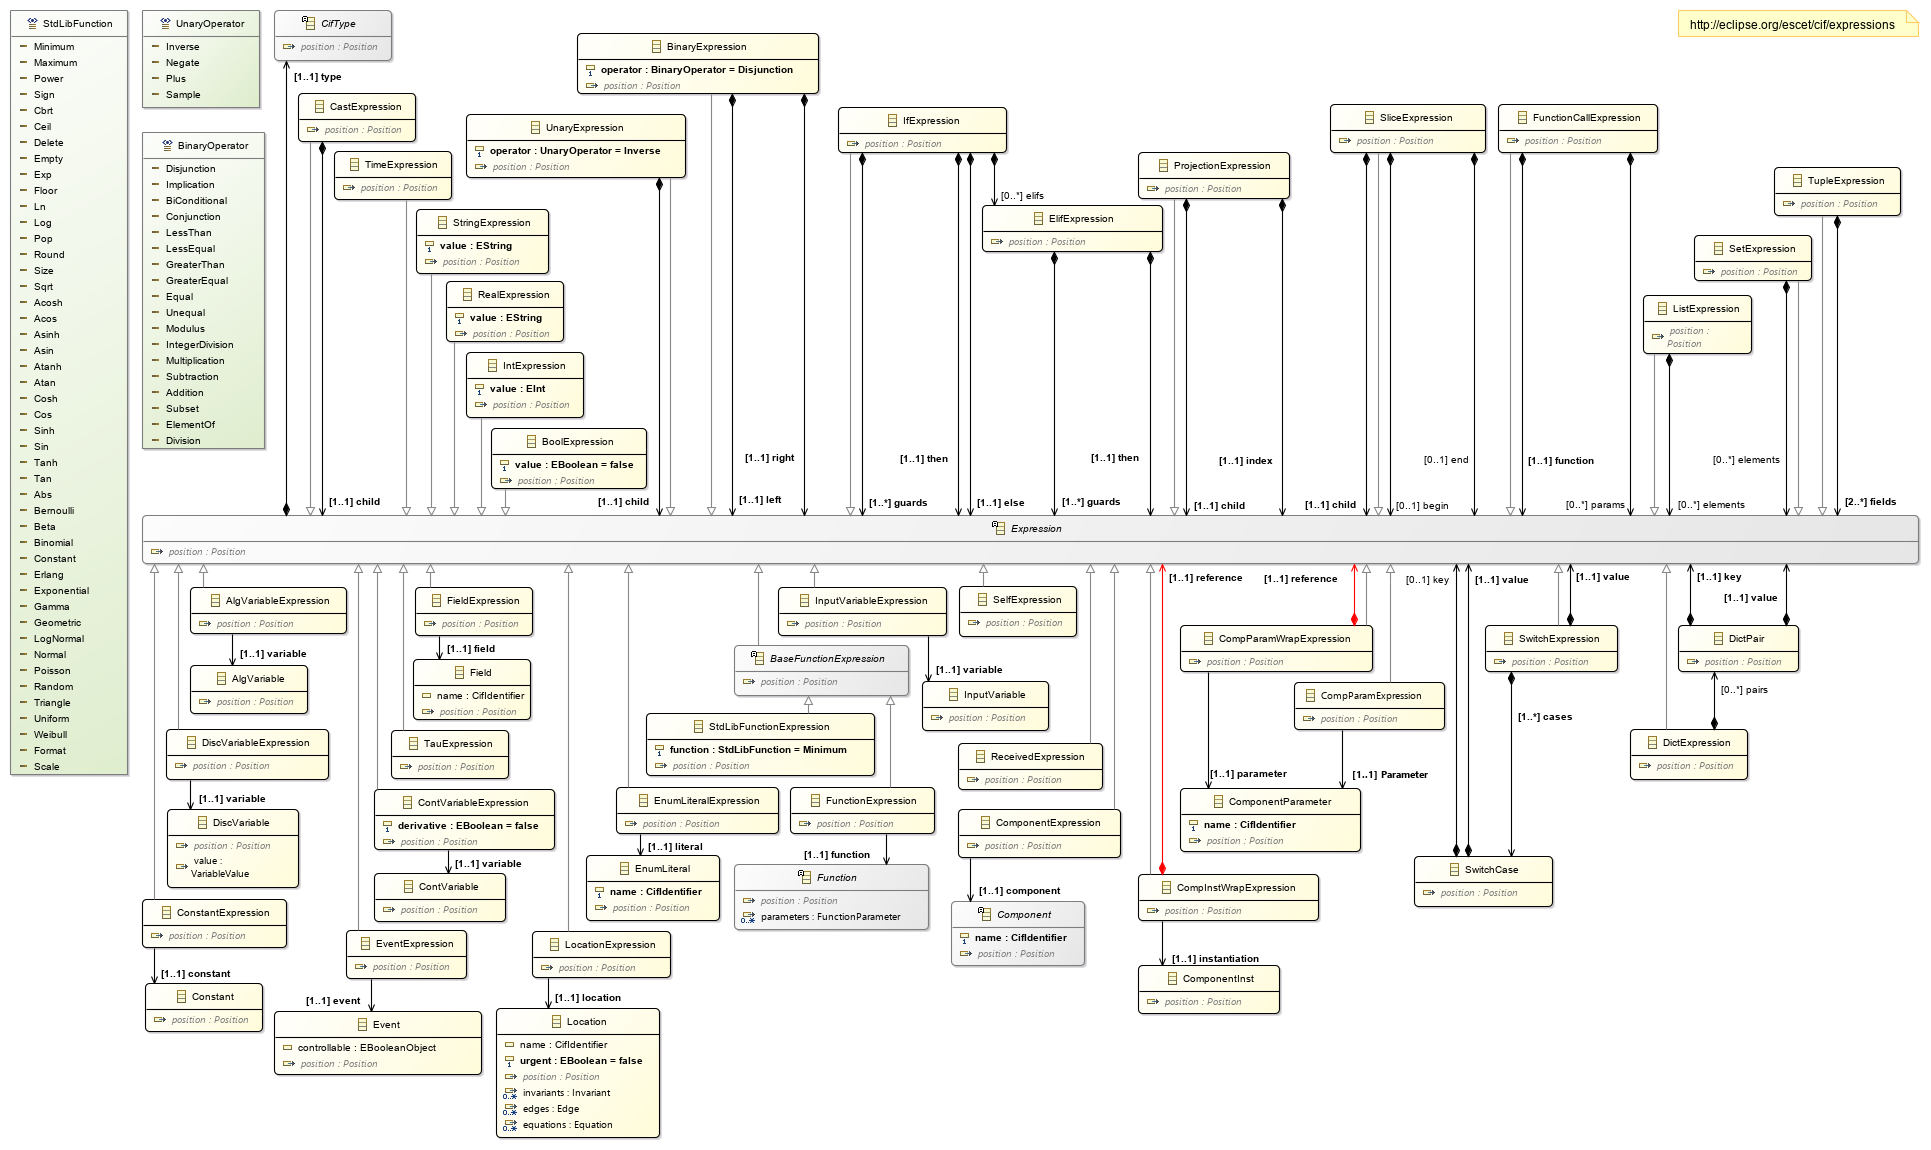
\includegraphics[angle=90,width=.8\textwidth]
                  {../model/images/expressions.png}
  \caption{\textit{expressions} package}\label{fig:pkg:expressions}
\end{figure}

Figure~\ref{fig:pkg:expressions} shows the \textit{expressions} package.
This package contains expression classes, and is pretty standard compared to
other languages.

The \cifclass{Expression} class is the main class. Note that all expressions
have a mandatory type. The derived classes above the \cifclass{Expression}
class represent literals, operators, collections, etc.

The derived classes below \cifclass{Expression} all deal with references to
objects in the CIF language. Of particular interest may be the
\cifclass{CompParamWrapExpression} and \cifclass{CompInstWrapExpression}
classes. They are used to keep track of references via component parameters
and component instantiations. See also Section~\ref{sec:scoping}.
}

% BinaryOperator (enumeration)
\newcommand{\enumdocuBinaryOperator}{
Binary operators for the \cifclass{BinaryExpression}. Type constraints are
listed in the \cifclass{BinaryExpression} class documentation.
}

\newcommand{\enumlitdocuBinaryOperatorAddition}{
Integer addition binary operator ($+$), as well as list concatenation, string
concatenation, and dictionary update.
}

\newcommand{\enumlitdocuBinaryOperatorBiConditional}{
Logical biconditional (or `if and only if') binary operator
($\Leftrightarrow$).
}

\newcommand{\enumlitdocuBinaryOperatorConjunction}{
Logical conjunction binary operator ($\land$), as well as set intersection
($\cap$).

Note that even though expressions are side effect free, evaluation may still
fail. Implementations must guarantee short circuit evaluation of this operator.
Note that when manipulating expressions, the operands may only be switched if
the resulting expression evaluates to the same value as the original expression
did, when using short circuit evaluation semantics for both the original and
resulting expression.
}

\newcommand{\enumlitdocuBinaryOperatorDisjunction}{
Logical disjunction binary operator ($\lor$), as well as set union ($\cup$).

Note that even though expressions are side effect free, evaluation may still
fail. Implementations must guarantee short circuit evaluation of this operator.
Note that when manipulating expressions, the operands may only be switched if
the resulting expression evaluates to the same value as the original expression
did, when using short circuit evaluation semantics for both the original and
resulting expression.
}

\newcommand{\enumlitdocuBinaryOperatorDivision}{
Real division binary operator ($/$).

Division by zero is considered a run-time error.
}

\newcommand{\enumlitdocuBinaryOperatorElementOf}{
Element-of binary operator ($\in$).
}

\newcommand{\enumlitdocuBinaryOperatorEqual}{
Equality binary operator ($=$).
}

\newcommand{\enumlitdocuBinaryOperatorGreaterEqual}{
Greater than or equal comparison binary operator ($\geq$).
}

\newcommand{\enumlitdocuBinaryOperatorGreaterThan}{
Greater than comparison binary operator ($>$).
}

\newcommand{\enumlitdocuBinaryOperatorImplication}{
Logical implication (or material condition, or material implication) binary
operator ($\Rightarrow$).

Note that even though expressions are side effect free, evaluation may still
fail. Implementations must guarantee short circuit evaluation of this operator.
Note that when manipulating expressions, the operands may only be switched if
the resulting expression evaluates to the same value as the original expression
did, when using short circuit evaluation semantics for both the original and
resulting expression.
}

\newcommand{\enumlitdocuBinaryOperatorIntegerDivision}{
Integer division binary operator ($\mathrm{div}$). Note that this operator has
the truncated division, or round towards zero, semantics.

\begin{tabular}{|l|l|l|l|} \hline
$\boldsymbol{a}$ & $\boldsymbol{b}$
                 & $\boldsymbol{a}~\boldsymbol{\mathrm{div}}~\boldsymbol{b}$
                 & $\boldsymbol{a} \boldsymbol{\bmod} \boldsymbol{b}$ \\ \hline
$7$   & $4$   & $1$   & $3$  \\
$7$   & $-4$  & $-1$  & $3$ \\
$-7$  & $4$   & $-1$  & $-3$  \\
$-7$  & $-4$  & $1$   & $-3$ \\
\hline\end{tabular}

Division by zero is considered a run-time error.
}

\newcommand{\enumlitdocuBinaryOperatorLessEqual}{
Less than or equal comparison binary operator ($\leq$).
}

\newcommand{\enumlitdocuBinaryOperatorLessThan}{
Less than comparison binary operator ($<$).
}

\newcommand{\enumlitdocuBinaryOperatorModulus}{
Integer modulus binary operator ($\bmod$). Note that
$a \bmod b \equiv a - b\cdot(a~\mathrm{div}~b)$. The result has the same sign
as the divident (the first operand).
For examples, see the \emph{IntegerDivision} binary operator.

It is considered a run-time error if the second operand evaluates to zero.
}

\newcommand{\enumlitdocuBinaryOperatorMultiplication}{
Multiplication binary operator ($*$).
}

\newcommand{\enumlitdocuBinaryOperatorSubset}{
Subset binary operator ($\subseteq$).
}

\newcommand{\enumlitdocuBinaryOperatorSubtraction}{
Subtraction binary operator ($-$), as well as set difference ($\setminus$), and
dictionary update.
}

\newcommand{\enumlitdocuBinaryOperatorUnequal}{
Inequality binary operator ($\not=$).
}

% StdLibFunction (enumeration)
\newcommand{\enumdocuStdLibFunction}{
Standard library functions. Parameter types and return types are listed in the
\cifclass{StdLibFunctionExpression} class documentation.
}

\newcommand{\enumlitdocuStdLibFunctionAbs}{
Absolute value function: $abs(x) = |x|$.
}

\newcommand{\enumlitdocuStdLibFunctionAcos}{
Arc cosine function, with a result in the range \range{0}{\pi}.

It is considered a run-time error if evaluation of the absolute value of the
argument results in a number larger than one.
}

\newcommand{\enumlitdocuStdLibFunctionAcosh}{
Inverse hyperbolic cosine function.
}

\newcommand{\enumlitdocuStdLibFunctionAsin}{
Arc sine function, with a result in the range \range{-\pi/2}{\pi/2}.

It is considered a run-time error if evaluation of the absolute value of the
argument results in a number larger than one.
}

\newcommand{\enumlitdocuStdLibFunctionAsinh}{
Inverse hyperbolic sine function.
}

\newcommand{\enumlitdocuStdLibFunctionAtan}{
Arc tangent function, with a result in the range \range{-\pi/2}{\pi/2}.
}

\newcommand{\enumlitdocuStdLibFunctionAtanh}{
Inverse hyperbolic tangent function.
}

\newcommand{\enumlitdocuStdLibFunctionBernoulli}{
Bernoulli distribution function.
}

\newcommand{\enumlitdocuStdLibFunctionBeta}{
Beta distribution function.
}

\newcommand{\enumlitdocuStdLibFunctionBinomial}{
Binomial distribution function.
}

\newcommand{\enumlitdocuStdLibFunctionCbrt}{
Cubic root function: $cbrt(x) = \sqrt[3]{x}$.
}

\newcommand{\enumlitdocuStdLibFunctionCeil}{
Ceiling function. Rounds up (towards $\infty$). In other words, results in the
smallest integer value that is not less than the argument.
}

\newcommand{\enumlitdocuStdLibFunctionConstant}{
Constant distribution function (useful for debugging/testing).
}

\newcommand{\enumlitdocuStdLibFunctionCos}{
Cosine function, with angle given in radians.
}

\newcommand{\enumlitdocuStdLibFunctionCosh}{
Hyperbolic cosine function: $cosh(x) = (e^{x}+e^{-x})/2$.
}

\newcommand{\enumlitdocuStdLibFunctionDelete}{
Delete function, to remove an element from a list, by using a zero-based index.
Negative indices count from the end of the list backwards.

It is considered a run-time error if an index is out of range for the list.
}

\newcommand{\enumlitdocuStdLibFunctionEmpty}{
Empty function, to check whether containers are empty.
}

\newcommand{\enumlitdocuStdLibFunctionErlang}{
Erlang distribution function.
}

\newcommand{\enumlitdocuStdLibFunctionExp}{
Exponential function: $exp(x) = e^x$.
}

\newcommand{\enumlitdocuStdLibFunctionExponential}{
Exponential distribution function.
}

\newcommand{\enumlitdocuStdLibFunctionFloor}{
Floor function. Rounds down (towards $-\infty$). In other words, results in the
largest integer value that is not exceed the argument.
}

\newcommand{\enumlitdocuStdLibFunctionFormat}{
Formatting function. Applies a format pattern (first argument, string literal)
to the remaining arguments.
}

\newcommand{\enumlitdocuStdLibFunctionGamma}{
Gamma distribution function.
}

\newcommand{\enumlitdocuStdLibFunctionGeometric}{
Geometric distribution function.
}

\newcommand{\enumlitdocuStdLibFunctionLn}{
Natural logarithmic function.

It is considered a run-time error if evaluation of the argument results in a
non-positive number.
}

\newcommand{\enumlitdocuStdLibFunctionLog}{
Logarithmic (base 10) function.

It is considered a run-time error if evaluation of the argument results in a
non-positive number.
}

\newcommand{\enumlitdocuStdLibFunctionLogNormal}{
Log-normal distribution function.
}

\newcommand{\enumlitdocuStdLibFunctionMaximum}{
Maximum value function:
$max(x, y) = \begin{cases}
             x & \text{if~} x >= y, \\
             y & \text{if~} x < y.
             \end{cases}$
}

\newcommand{\enumlitdocuStdLibFunctionMinimum}{
Minimum value function:
$min(x, y) = \begin{cases}
             x & \text{if~} x <= y, \\
             y & \text{if~} x > y.
             \end{cases}$
}

\newcommand{\enumlitdocuStdLibFunctionNormal}{
Normal distribution function.
}

\newcommand{\enumlitdocuStdLibFunctionPoisson}{
Poisson distribution function.
}

\newcommand{\enumlitdocuStdLibFunctionPop}{
Pops the first element from a list, and returns a tuple of the element and the
list without that element.

It is considered a run-time error if the list is empty.
}

\newcommand{\enumlitdocuStdLibFunctionPower}{
Power (exponentiation) function: $pow(a, b) = a^b$. Note that $0^0 = 1$.

It is considered a run-time error if one of the following conditions holds
during evaluation:
\begin{itemize}
\item the base is zero, and the exponent is negative,
\item the base is negative, and the exponent is a non-integer number.
\end{itemize}
}

\newcommand{\enumlitdocuStdLibFunctionRandom}{
Random (standard uniform) distribution function.
}

\newcommand{\enumlitdocuStdLibFunctionRound}{
Round function. Rounds to the nearest integer value. If the value is exactly
between two integer values, it is rounded up (towards $\infty$). That is:
$round(x) = \left\lfloor x + 0.5 \right\rfloor$.
}

\newcommand{\enumlitdocuStdLibFunctionScale}{
Linear scaling with offset. A value $v$ is interpreted in input interval
\range{inmin}{inmax}, and transformed to a value in output interval
\range{outmin}{outmax}:

$scale(v, inmin, inmax, outmin, outmax) =
outmin + fraction * (outmax - outmin)$ \\
with $fraction = (v - inmin) / (inmax - inmin)$

The intervals may be increasing or decreasing. The input value does not have
to be included in the input interval. In that case it helps to think of the
function as applying a linear transformation.

It is considered a run-time error if the input interval is empty
($inmin = inmax$), as that leads to division by zero.
}

\newcommand{\enumlitdocuStdLibFunctionSign}{
Sign (or signum) function:
$sign(x) = \begin{cases}
           -1 & \text{if~} x < 0, \\
           0  & \text{if~} x = 0, \\
           1  & \text{if~} x > 0.
           \end{cases}$
}

\newcommand{\enumlitdocuStdLibFunctionSin}{
Sine function, with angle given in radians.
}

\newcommand{\enumlitdocuStdLibFunctionSinh}{
Hyperbolic sine function: $sinh(x) = (e^{x}-e^{-x})/2$.
}

\newcommand{\enumlitdocuStdLibFunctionSize}{
Function to get the size of a string, list, set, or dictionary.
}

\newcommand{\enumlitdocuStdLibFunctionSqrt}{
Square root function: $sqrt(x) = \sqrt x$.

It is a run-time error if the argument evaluates to a negative number.
}

\newcommand{\enumlitdocuStdLibFunctionTan}{
Tangent function, with angle given in radians.
}

\newcommand{\enumlitdocuStdLibFunctionTanh}{
Hyberbolic tangent function: $tanh(x) = sinh(x)/cosh(x)$.
}

\newcommand{\enumlitdocuStdLibFunctionTriangle}{
Triangle distribution function.
}

\newcommand{\enumlitdocuStdLibFunctionUniform}{
Uniform distribution function.
}

\newcommand{\enumlitdocuStdLibFunctionWeibull}{
Weibull distribution function.
}

% UnaryOperator (enumeration)
\newcommand{\enumdocuUnaryOperator}{
Unary operators for the \cifclass{UnaryExpression}. Type constraints are
listed in the \cifclass{UnaryExpression} class documentation.
}

\newcommand{\enumlitdocuUnaryOperatorInverse}{
Logical inverse unary operator ($\lnot$).
}

\newcommand{\enumlitdocuUnaryOperatorNegate}{
Numerical negation (or additive inverse, or opposite) unary operator ($-$).
}

\newcommand{\enumlitdocuUnaryOperatorPlus}{
Numerical plus unary operator ($+$). Identity operator.
}

\newcommand{\enumlitdocuUnaryOperatorSample}{
Sample unary operator. Draws a sample from a stochastic distribution, resulting
in a tuple, with the sampled value, and the original distribution with a
modified seed.
}

% AlgVariableExpression (class)
\newcommand{\clsdocuAlgVariableExpression}{
An algebraic variable reference expression.

\begin{constraints}
\citem{AlgVariableExpression.type}
  The type of this expression must match the type of the referenced algebraic
  variable. For ranged types, the range of the type of this expression must
  be equal to the range of the type of the algebraic variable, if it is
  specified.
\end{constraints}
}

\newcommand{\featdocuAlgVariableExpressionvariable}{
The referenced algebraic variable.

\begin{constraints}
\citem{AlgVariableExpression.variableInScope}
  The algebraic variable reference must satisfy the scoping rules.
\end{constraints}
}

% BaseFunctionExpression (abstract class)
\newcommand{\clsdocuBaseFunctionExpression}{
Base class for function reference expressions.
}

% BinaryExpression (class)
\newcommand{\clsdocuBinaryExpression}{
A binary expression.

\begin{constraints}
\citem{BinaryExpression.type}
  The types of the left child expression, right child expression, and the type
  of the binary expression itself (the result type), depend on the
  \cifclass{BinaryOperator}. Table~\ref{tbl:bin-expr-types}
  lists the allowed combinations.

  Note that for the \cifenumlit{BinaryOperator.Equal} and
  \cifenumlit{BinaryOperator.Unequal} binary operators, the types of the
  left and right child expressions must be equal. However, component types
  and component definition types, as well as function and distribution types,
  are not allowed, as those types don't support value equality. For ranged
  types, the ranges are ignored.

  Note that for the \cifenumlit{BinaryOperator.ElementOf} binary operator,
  the type of the left child expressions must not be a component type, a
  component definition type, a function type, or a distribution types,
  as those types don't support value equality. For ranged types, the ranges
  are ignored.

  For the \cifenumlit{BinaryOperator.Modulus} binary operator, the result
  range calculation is simplified, leading not only to simpler calculations,
  but also to more intuitive result ranges. It does however result in larger
  result ranges (over-approximations).

  For integer types, if one of the operands has a rangeless integer type,
  the result type is also rangeless, if the result type is an integer type as
  well.

  For list types, if one of the operands is an array, we try to keep the result
  an array as well. However, over approximations are sometimes used for the
  result types.
\citem{BinaryExpression.divideByZero}
  For the \cifenumlit{BinaryOperator.IntegerDivision} and
  \cifenumlit{BinaryOperator.Modulus} binary operators, if the
  right child expression has an integer type with range \range{0}{0}, then
  the model is invalid, as this can only result in a division by zero run-time
  evaluation error.
\end{constraints}

\begin{table}
  \small
  \centering
  \begin{tabular}{l l l l}
    \textbf{Operator} & \textbf{Left type} & \textbf{Right type}
                      & \textbf{Result type} \\
    \hline
    Implication     & bool  & bool  & bool \\
    BiConditional   & bool  & bool  & bool \\
    Disjunction     & bool  & bool  & bool \\
                    & set t & set t & set t \\
    Conjunction     & bool  & bool  & bool \\
                    & set t & set t & set t \\
    LessThan        & int / real & int / real & bool \\
    LessEqual       & int / real & int / real & bool \\
    GreaterThan     & int / real & int / real & bool \\
    GreaterEqual    & int / real & int / real & bool \\
    Equal           & $t$ & $t$ & bool \\
    Unequal         & $t$ & $t$ & bool \\
    Addition        & int \range{l_1}{u_1} &
                      int \range{l_2}{u_2} &
                      int \range{l_1 + l_2}{u_1 + u_2} \\
                    & int & int & int \\
                    & int & real & real \\
                    & real & int & real \\
                    & real & real & real \\
                    & list t & list t & list t \\
                    & list \range{l_1}{u_1} t &
                      list \range{l_2}{u_2} t &
                      list \range{l_1 + l_2}{u_1 + u_2} t \\
                    & string & string & string \\
                    & dict(k:v) & dict(k:v) & dict(k:v) \\
    Subtraction     & int \range{l_1}{u_1} &
                      int \range{l_2}{u_2} &
                      int \range{l_1 - u_2}{u_1 - l_2} \\
                    & int & int & int \\
                    & int & real & real \\
                    & real & int & real \\
                    & real & real & real \\
                    & set t & set t & set t \\
                    & dict(k:v) & dict(k:v) & dict(k:v) \\
                    & dict(k:v) & set k & dict(k:v) \\
                    & dict(k:v) & list k & dict(k:v) \\
                    & dict(k:v) & list \range{l}{u} k & dict(k:v) \\[3pt]
    Multiplication  & int \range{l_1}{u_1} &
                      int \range{l_2}{u_2} &
                      int \rangeBig
                            {\mathrm{min}\left(
                             \begin{array}{@{}r@{\,}c@{\,}r@{}l@{}}
                                 l_1 & \cdot & l_2 & , \\
                                 l_1 & \cdot & u_2 & , \\
                                 u_1 & \cdot & l_2 & , \\
                                 u_1 & \cdot & u_2
                             \end{array}
                             \right)
                            }
                            {\mathrm{max}\left(
                             \begin{array}{@{}r@{\,}c@{\,}r@{}l@{}}
                                 l_1 & \cdot & l_2 & , \\
                                 l_1 & \cdot & u_2 & , \\
                                 u_1 & \cdot & l_2 & , \\
                                 u_1 & \cdot & u_2
                             \end{array}
                             \right)
                            } \\[20pt]
                    & int  & int  & int \\
                    & int  & real & real \\
                    & real & int  & real \\
                    & real & real & real \\
    Division        & int / real & int / real & real \\
    IntegerDivision & int \range{l_1}{u_1} &
                      int \range{l_2}{u_2} &
                      int \rangeV
                            {\mathrm{min}\{x~\mathrm{div}~y~|~
                                           x \in \mathrange{l_1}{u_1},
                                           y \in \mathrange{l_2}{u_2},
                                           y \neq 0
                                         \}}
                            {\mathrm{max}\{x~\mathrm{div}~y~|~
                                           x \in \mathrange{l_1}{u_1},
                                           y \in \mathrange{l_2}{u_2},
                                           y \neq 0
                                         \}} \\[10pt]
                    & int & int & int \\
    Modulus         & int \range{l_1}{u_1} &
                      int \range{l_2}{u_2} &
                      int
                      \rangeV
                       {\left(
                        \begin{array}{@{}rl@{}}
                          \mathrm{min}(0, -\mathrm{max}(|l_2|, |u_2|) + 1)
                                  & \text{if~} l_1 <    0 \\
                          0       & \text{if~} l_1 \geq 0
                        \end{array}
                        \right)}
                       {\left(
                        \begin{array}{@{}rl@{}}
                          \mathrm{max}(0,  \mathrm{max}(|l_2|, |u_2|) - 1)
                                  & \text{if~} u_1 \geq 0 \\
                          0       & \text{if~} u_1 <    0
                        \end{array}
                        \right)}\\[5pt]
                    & int & int & int \\
    ElementOf       & t & list t & bool \\
                    & t & list \range{l}{u} t & bool \\
                    & t & set t & bool \\
                    & k & dict(k:v) & bool \\
    Subset          & set t & set t & bool \\
    \hline
  \end{tabular}
  \caption{Binary expression type constraints.}
  \label{tbl:bin-expr-types}
\end{table}
}

\newcommand{\featdocuBinaryExpressionleft}{
The left child of the binary expression.
}

\newcommand{\featdocuBinaryExpressionoperator}{
The binary operator of the binary expression.
}

\newcommand{\featdocuBinaryExpressionright}{
The right child of the binary expression.
}

% BoolExpression (class)
\newcommand{\clsdocuBoolExpression}{
A boolean value literal expression.

\begin{constraints}
\citem{BoolExpression.type}
  The type of a boolean expression must be a boolean type.
\end{constraints}
}

\newcommand{\featdocuBoolExpressionvalue}{
The boolean value.
}

% CastExpression (class)
\newcommand{\clsdocuCastExpression}{
Cast expression.

It is considered a run-time error if casting from a string value, and the
string value is not a valid textual representation of a value for the result
type.

\begin{constraints}
\citem{CastExpression.type}
  The types of the child expression and the cast expression itself must match.
  For $t$ to $t$ casts, the types must be exactly equal. That is, for ranged
  types the ranges must be equal as well. Table~\ref{tbl:cast-expr-types} lists
  the allowed combinations.
\end{constraints}

\begin{table}
  \centering
  \begin{tabular}{l l l l}
    \textbf{Child type} & \textbf{Cast/result type} \\
    \hline
    int & real \\
    int & string \\
    real & string \\
    bool & string \\
    string & int (rangeless) \\
    string & real \\
    string & bool \\
    automaton reference (including `self') & string \\
    t & t \\
    \hline
  \end{tabular}
  \caption{Cast expression type constraints.}
  \label{tbl:cast-expr-types}
\end{table}
}

\newcommand{\featdocuCastExpressionchild}{
The child of the cast expression.
}

% CompInstWrapExpression (class)
\newcommand{\clsdocuCompInstWrapExpression}{
Component instantiation reference wrapping expression. Allows keeping track
of references via component instantiations. Similar to the
\cifclass{CompInstWrapType} class, but for expression references instead of
type references. Similar to the \cifclass{CompParamWrapExpression} class,
but for references via component instantiations instead of via component
parameters. See also Section~\ref{sec:scoping}.

\begin{constraints}
\citem{CompInstWrapExpression.type}
  The type of the component instantiation reference wrapping expression
  must be equal to the type of its reference expression.
\end{constraints}
}

\newcommand{\featdocuCompInstWrapExpressioninstantiation}{
The component instantiation via which the object is referenced.

\begin{constraints}
\citem{CompInstWrapExpression.noCompDefBody}
  Components instantiations that are bodies of component definitions may not
  be referenced here, as the body \emph{is} the component definition.
\citem{CompInstWrapExpression.instantiationInScope}
  The component instantiation reference must satisfy the scoping rules.
\end{constraints}
}

\newcommand{\featdocuCompInstWrapExpressionreference}{
The object that is referenced via a component instantiation.

This feature contains \cifclass{Expression} instances, to allow for wrapping
expressions to be used.

\begin{constraints}
\citem{CompInstWrapExpression.reference}
  The \emph{reference} expression must be a reference.
\end{constraints}
}

% CompParamExpression (class)
\newcommand{\clsdocuCompParamExpression}{
A component parameter reference expression.

\begin{constraints}
\citem{CompParamExpression.type}
  The type of the component parameter reference expression must match the
  type of the referenced component parameter.
\end{constraints}
}

\newcommand{\featdocuCompParamExpressionparameter}{
The referenced component parameter.

\begin{constraints}
\citem{CompParamExpression.parameterInScope}
  The component parameter must satisfy the scoping rules.
\end{constraints}
}

% CompParamWrapExpression (class)
\newcommand{\clsdocuCompParamWrapExpression}{
Component parameter reference wrapping expression. Allows keeping track
of references via component parameters. Similar to the
\cifclass{CompParamWrapType} class, but for expression references instead of
type references. Similar to the \cifclass{CompInstWrapExpression} class,
but for references via component parameters instead of via component
instantiations. See also Section~\ref{sec:scoping}.

\begin{constraints}
\citem{CompParamWrapExpression.type}
  The type of the component parameter reference wrapping expression
  must be equal to the type of its reference expression.
\end{constraints}
}

\newcommand{\featdocuCompParamWrapExpressionparameter}{
The component parameter via which the object is referenced.

\begin{constraints}
\citem{CompParamWrapExpression.parameterInScope}
  The component parameter reference must satisfy the scoping rules.
\end{constraints}
}

\newcommand{\featdocuCompParamWrapExpressionreference}{
The object that is referenced via a component parameter.

This feature contains \cifclass{Expression} instances, to allow for wrapping
expressions to be used.

\begin{constraints}
\citem{CompParamWrapExpression.reference}
  The \emph{reference} expression must be a reference.
\end{constraints}
}

% ComponentExpression (class)
\newcommand{\clsdocuComponentExpression}{
A component reference expression.

\begin{constraints}
\citem{ComponentExpression.type}
  The type of the component reference expression must be a component type that
  refers to the same component as this expression does.
\end{constraints}
}

\newcommand{\featdocuComponentExpressioncomponent}{
The referenced component.

\begin{constraints}
\citem{ComponentExpression.noCompDefBody}
  Components that are bodies of component definitions may not be referenced
  here, as the body \emph{is} the component definition.
\citem{ComponentExpression.noSpec}
  Specifications, which are technically components, may not be referenced here,
  as they serve as outer grouping only. Note that in the CIF textual syntax,
  they can't be referenced either, as they don't have a name.
\citem{ComponentExpression.componentInScope}
  The component reference must satisfy the scoping rules.
\end{constraints}
}

% ConstantExpression (class)
\newcommand{\clsdocuConstantExpression}{
A constant reference expression.

\begin{constraints}
\citem{ConstantExpression.type}
  The type of this expression must match the type of the referenced constant.
  For ranged types, the range of the type of this expression must be equal to
  the range of the type of the constant, if specified.
\end{constraints}
}

\newcommand{\featdocuConstantExpressionconstant}{
The referenced constant.

\begin{constraints}
\citem{ConstantExpression.constantInScope}
  The constant reference must satisfy the scoping rules.
\end{constraints}
}

% ContVariableExpression (class)
\newcommand{\clsdocuContVariableExpression}{
A continuous variable reference expression.

\begin{constraints}
\citem{ContVariableExpression.type}
  The type of the variable reference expression must be a real type.
\end{constraints}
}

\newcommand{\featdocuContVariableExpressionderivative}{
Indicates whether this reference is a reference to the derivative of the
variable (\emph{true}) or to the variable itself (\emph{false}).
}

\newcommand{\featdocuContVariableExpressionvariable}{
The referenced continuous variable.

\begin{constraints}
\citem{ContVariableExpression.variableInScope}
  The continuous variable reference must satisfy the scoping rules.
\end{constraints}
}

% DictExpression (class)
\newcommand{\clsdocuDictExpression}{
A dictionary literal expression.

It is considered a run-time error if a dictionary literal has duplicate keys.

\begin{constraints}
\citem{DictExpression.type}
  The type of the dictionary expression must be a dictionary type. Each of the
  keys of the pairs must match the key type of the dictionary type. Each of the
  values of the pairs must match the value type of the dictionary type. For
  ranged types, the ranges (if specified) of the keys and values must be
  contained in the range of the key type and value type respectively.
\end{constraints}
}

\newcommand{\featdocuDictExpressionpairs}{
The key/value pairs of the dictionary.
}

% DictPair (class)
\newcommand{\clsdocuDictPair}{
A single key/value pair for a \cifclass{DictExpression}.
}

\newcommand{\featdocuDictPairkey}{
The key of the key/value pair.
}

\newcommand{\featdocuDictPairvalue}{
The value of the key/value pair.
}

% DiscVariableExpression (class)
\newcommand{\clsdocuDiscVariableExpression}{
A discrete variable reference expression.

\begin{constraints}
\citem{DiscVariableExpression.type}
  The type of the discrete variable reference expression must match the type
  of the referenced discrete variable. For ranged types, the ranges (if
  specified) must be equal.
\end{constraints}
}

\newcommand{\featdocuDiscVariableExpressionvariable}{
The referenced discrete variable.

\begin{constraints}
\citem{DiscVariableExpression.variableInScope}
  The discrete variable reference must satisfy the scoping rules.
\end{constraints}
}

% ElifExpression (class)
\newcommand{\clsdocuElifExpression}{
An `elif' (`else-if') alternative of an \cifclass{IfExpression}.
}

\newcommand{\featdocuElifExpressionguards}{
The guard predicates for this alternative.

If multiple predicates are given, this feature represents the logical
conjunction of those predicates. Note that this represents the mathematical
conjunction, and not the short-circuit conjunction binary operator. As such,
there is no ordering between the guards.

\begin{constraints}
\citem{ElifExpression.guardTypes}
  The guard predicates must have boolean types.
\end{constraints}
}

\newcommand{\featdocuElifExpressionthen}{
The value that the \cifclass{IfExpression} evaluates to if the `guard'
evaluates to \emph{true}.
}

% EnumLiteralExpression (class)
\newcommand{\clsdocuEnumLiteralExpression}{
An enumeration literal reference expression.

\begin{constraints}
\citem{EnumLiteralExpression.type}
  The type of an enumeration literal expression must be equal to the
  enumeration that the literal is a part of.
\end{constraints}
}

\newcommand{\featdocuEnumLiteralExpressionliteral}{
The referenced enumeration literal.

\begin{constraints}
\citem{EnumLiteralExpression.literalInScope}
  The enumeration literal reference must satisfy the scoping rules.
\end{constraints}
}

% EventExpression (class)
\newcommand{\clsdocuEventExpression}{
An event reference expression.

Only used for event references, as events can't be used in a value context. It
is part of the expression tree, to allow wrapping expressions to be used. See
also Section~\ref{sec:scoping}.

Can not be used to refer to the `tau' event.

\begin{constraints}
\citem{EventExpression.type}
  The type of an event expression must be a boolean type.
\end{constraints}
}

\newcommand{\featdocuEventExpressionevent}{
The referenced event.

\begin{constraints}
\citem{EventExpression.eventInScope}
  The event reference must satisfy the scoping rules.
\citem{EventExpression.occurrence}
  Events may only be used in places where they are directly used as event
  reference (such as events on edges, in alphabets, in monitor sets, in
  component instantiation arguments for event parameters, etc). They may thus
  explicitly not be used in functions, guards, initial values of variables,
  etc.
\end{constraints}
}

% Expression (abstract class)
\newcommand{\clsdocuExpression}{
Base class for all CIF expressions.
}

\newcommand{\featdocuExpressiontype}{
The type of the expression.
}

% FieldExpression (class)
\newcommand{\clsdocuFieldExpression}{
A tuple field reference expression.

\begin{constraints}
\citem{FieldExpression.occurrence}
  Instances of \emph{FieldExpression} may only occur in the \emph{index}
  feature of the \cifclass{ProjectionExpression} class. They must not be
  wrapped in other expressions.
\citem{FieldExpression.type}
  The type of a field expression must be an integer type, with as range the
  single value that corresponds to the 0-based index of the field in the tuple
  type of which it is a part.
\end{constraints}
}

\newcommand{\featdocuFieldExpressionfield}{
The referenced tuple field.

\begin{constraints}
\citem{FieldExpression.fieldInScope}
  The field reference must satisfy the scoping rules. For the details, see the
  \cifclass{ProjectionExpression}.
\end{constraints}
}

% FunctionCallExpression (class)
\newcommand{\clsdocuFunctionCallExpression}{
A function call expression.

\begin{constraints}
\citem{FunctionCallExpression.type}
  The type of the function call expression must match the types of the function
  and its parameters. That is, the function must have a function type. The
  type of the functional call expression must match the result type of the
  function type. For ranged types, the ranges (if specified) must be equal.
  The count and types of the arguments must match the parameter types of the
  function type. For ranged types, the ranges (if specified) of the arguments
  must be contained in the ranges of the parameter types of the function type.
\end{constraints}
}

\newcommand{\featdocuFunctionCallExpressionarguments}{
The function arguments for the function call.
}

\newcommand{\featdocuFunctionCallExpressionfunction}{
The function to call.
}

% FunctionExpression (class)
\newcommand{\clsdocuFunctionExpression}{
A user-defined function reference expression.

\begin{constraints}
\citem{FunctionExpression.type}
  The type of a function reference expression must be a function type, with
  a return type matching the return type of the referenced function, and
  parameter types matching the types of the parameters of the referenced
  function. For ranged types, the ranges must match exactly.
\end{constraints}
}

\newcommand{\featdocuFunctionExpressionfunction}{
The referenced user-defined function.

\begin{constraints}
\citem{FunctionExpression.functionInScope}
  The function reference must satisfy the scoping rules.
\end{constraints}
}

% IfExpression (class)
\newcommand{\clsdocuIfExpression}{
A conditional expression.

\begin{constraints}
\citem{IfExpression.type}
  The type of the `then' expression, the type of the `else' expression,
  the types of the `thens' of the `elif' expressions (if any), and the type
  of this expression, must all match.

  Component and component definition types are not allowed.

  For integer types, for `then' range \range{lt}{ut}, for `else' range
  \range{le}{ue}, for `elif' ranges \range{{lf}_n}{{uf}_n}, in case of $n$
  `elif' alternatives, $0 < n$, the range of this expression must be equal to
  \range{lt \min le \min
              \left( \underset{0 \leq i < n}{\mathrm{min}}({lf}_i) \right)}
        {ut \max ue \max
              \left( \underset{0 \leq i < n}{\mathrm{max}}({uf}_i) \right)}.
  That is, the ranges are merged. Similarly, ranges for other ranged types are
  merged.

  Note that the guards of the alternatives are not taken into account. Also,
  if one of the alternatives has a non-ranged integer type, the result has a
  non-ranged integer type as well. Similar notes apply to other ranged types.
\end{constraints}
}

\newcommand{\featdocuIfExpressionelifs}{
The `elif' (`else-if') alternatives. Processed in order, if the `guard'
evaluates to \emph{false}.
}

\newcommand{\featdocuIfExpressionelse}{
The `else' value. Returned if no other alternative has a \emph{true} guard.
}

\newcommand{\featdocuIfExpressionguards}{
The guard predicates for the `then' value.

If multiple predicates are given, this feature represents the logical
conjunction of those predicates. Note that this represents the mathematical
conjunction, and not the short-circuit conjunction binary operator. As such,
there is no ordering between the guards.

\begin{constraints}
\citem{IfExpression.guardTypes}
  The guard predicates must have boolean types.
\end{constraints}
}

\newcommand{\featdocuIfExpressionthen}{
The `then' value. Returned if the `guard' evaluates to \emph{true}.
}

% InputVariableExpression (class)
\newcommand{\clsdocuInputVariableExpression}{
An input variable reference expression.

\begin{constraints}
\citem{InputVariableExpression.type}
  The type of this expression must match the type of the referenced input
  variable. For ranged types, the ranges (if specified) must be equal.
\end{constraints}
}

\newcommand{\featdocuInputVariableExpressionvariable}{
The referenced input variable.

\begin{constraints}
\citem{InputVariableExpression.variableInScope}
  The input variable reference must satisfy the scoping rules.
\end{constraints}
}

% IntExpression (class)
\newcommand{\clsdocuIntExpression}{
An integer value literal expression.

The value of integer value literal expressions is encoded using the \emph{EInt}
datatype, which matches 32-bit integers in the range \range{-2^{31}}{2^{31}-1}.
Note that integer values are also used for the bounds of ranges
(see \cifclass{IntType}), which means that both values and integer type
ranges are limited to that given range of integers.

Operations that result in overflow or underflow should be considered
errors, and under no circumstance should wrapping or saturation take place.

If operations depend only on integer types with ranges, we enforce that no
overflow can ever happen, by using static semantic constraints, as to avoid
run-time overflow detection. If one of the operands involves a rangeless
integer type, range checking is disabled for that operation, deferring the
responsibility to run-time, and thus the implementation.

\begin{constraints}
\citem{IntExpression.type}
  The type of an integer expression with value $v$ must be an integer type
  with range \range{v}{v}.
\end{constraints}
}

\newcommand{\featdocuIntExpressionvalue}{
The integer value. May be negative, zero, or positive.
}

% ListExpression (class)
\newcommand{\clsdocuListExpression}{
A list literal expression.

Operations that result in overflow on the sizes of lists should be considered
errors.

If operations depend only on list types with ranges, we enforce that no
out-of-range errors can ever happen, by using static semantic constraints, as
to avoid run-time out-of-range detection. If one of the operands involves a
rangeless list type, range checking is disabled for that operation, deferring
the responsibility to run-time, and thus the implementation.

\begin{constraints}
\citem{ListExpression.type}
  The type of the list expression must be a list type, with range \range{n}{n}
  for a list of $n$ elements. Each of the elements must match the element type
  of the list type. For ranged element types, the ranges (if specified) of the
  types of the elements must be contained in the range of the element type of
  the list type.
\end{constraints}
}

\newcommand{\featdocuListExpressionelements}{
The elements of the list.
}

% LocationExpression (class)
\newcommand{\clsdocuLocationExpression}{
A location reference expression. Represents an `is the location active'
boolean expression.

\begin{constraints}
\citem{LocationExpression.type}
  The type of a location expression must be a boolean type.
\end{constraints}
}

\newcommand{\featdocuLocationExpressionlocation}{
The referenced location.

\begin{constraints}
\citem{LocationExpression.locationInScope}
  The location reference must satisfy the scoping rules.
\end{constraints}
}

% ProjectionExpression (class)
\newcommand{\clsdocuProjectionExpression}{
Projection expression.

Lists can be indexed using a zero-based index. Negative indices count from
the end of the list backwards. It is considered a run-time error if an index
is out of range for the list.

Dictionaries can be indexed using keys. It is considered a run-time error if
a key is not in the dictionary. An exception is the last projection of an
addressable, as a new key/value pair is created if the key does not exist for
such a projection.

Strings can be indexed similar to lists.

Tuples can be indexed using a zero-based index. It is considered a run-time
error if an index is out of range (negative or greater than or equal to the
size of the tuple).

Tuples can also be indexed using field names. In such a case, the
\emph{index} expression must be a \cifclass{FieldExpression}, which must not
be wrapped by any other expressions.

\begin{constraints}
\citem{ProjectionExpression.type}
  The types of the child expression and the projection expression itself must
  match. Table~\ref{tbl:proj-expr-types} lists the allowed combinations.
\end{constraints}

\begin{table}
  \centering
  \begin{tabular}{l l l l}
    \textbf{Child type} & \textbf{Index (type)} &
      \textbf{Projection/result type} \\
    \hline
    list t & int & t \\
    list t & int[a..b] & t \\
    list \range{l}{u} t & int & t \\
    list \range{l}{u} t & int[a..b] & t \\
    dict(k:v) & k & v \\
    string & int & string \\
    tuple(t1 f1, t2 f2, \ldots, tn fn) & int i & ti \\
    tuple(t1 f1, t2 f2, \ldots, tn fn) & field fi & ti \\
    \hline
  \end{tabular}
  \caption{Projection expression type constraints.}
  \label{tbl:proj-expr-types}
\end{table}
}

\newcommand{\featdocuProjectionExpressionchild}{
The child expression of the projection expression. This is the value that is
being projected.
}

\newcommand{\featdocuProjectionExpressionindex}{
The projection index of the projection expression. This indicates what to
project from the child expression.

\begin{constraints}
\citem{ProjectionExpression.indexInScope}
  For projection on tuples, the fields of the tuple type of the child
  expression are in scope, and the fields take precedence over any other
  objects with those names, in the same scope.
\end{constraints}
}

% RealExpression (class)
\newcommand{\clsdocuRealExpression}{
A real number value literal expression.

\begin{constraints}
\citem{RealExpression.type}
  The type of a real expression must be a real type.
\end{constraints}
}

\newcommand{\featdocuRealExpressionvalue}{
The real number value. Note that real numbers are represented in the metamodel
as strings, to keep the original formatting, and to keep the precise value.
For details on the representation of real numbers in the implementation, see
the \cifclass{RealType} class.

The syntax of the strings is CIF textual syntax for real numbers. Note that
this explicitly excludes negative real numbers, which are real numbers with
a unary negation operator.
}

% ReceivedExpression (class)
\newcommand{\clsdocuReceivedExpression}{
A reference to the value received as part of a channel communication.

\begin{constraints}
\citem{ReceivedExpression.scope}
  The received value only exists in the updates of edges, for edges where a
  value is received. Received values may not be assigned (are read-only).
  They may be used on the right hand side of assignments, as projection indices
  in the addressables, and in guards for `if' updates.
\citem{ReceivedExpression.type}
  The type of a received value reference expression must have the same type as
  the type of the event or events over which data is communicated. If multiple
  events are present on the edge, they must have equal types. If communication
  over a \cifclass{VoidType} channel is performed, the received value does not
  exist, as there a no values for `void' types.
\end{constraints}
}

% SelfExpression (class)
\newcommand{\clsdocuSelfExpression}{
A self reference to an automaton or automaton definition.

\begin{constraints}
\citem{SelfExpression.scope}
  The self expression may only be used within automata and automaton
  definitions.
\citem{SelfExpression.type}
  The type of a self expression must be an automaton type or automaton
  definition type, referring to the automaton or automaton definition in which
  the self expression is used.
\end{constraints}
}

% SetExpression (class)
\newcommand{\clsdocuSetExpression}{
A set literal expression.

\begin{constraints}
\citem{SetExpression.type}
  The type of the set expression must be a set type. Each of the
  elements must match the element type of the set type. For ranged element
  types, the ranges (if specified) of the types of the elements must be
  contained in the range of the element type of the set type.
\end{constraints}
}

\newcommand{\featdocuSetExpressionelements}{
The elements of the set.
}

% SliceExpression (class)
\newcommand{\clsdocuSliceExpression}{
Slice expression.

Lists can also be sliced, using a $begin$ and $end$ index. This results in a
part of the original list, for the sub-range \range{begin}{end-1}. Both indices
are optional. An omitted $begin$ index equals $0$, and an omitted $end$ index
equals the length of the list. Indices may be negative to count from the end
of the list backwards. Out of range slice indices are handled gracefully. An
index that is too large is replaced by the list size. A lower bound larger
than the upper bound results in an empty list. This applies to negative
indices as well.

Strings can be sliced similar to lists.

\begin{constraints}
\citem{SliceExpression.type}
  The types of the child expression and the slice expression itself must
  match. Table~\ref{tbl:slice-expr-types} lists the allowed combinations.
\end{constraints}

\begin{table}
  \centering
  \begin{tabular}{l l l l}
    \textbf{Child type} & \textbf{begin} & \textbf{end} &
      \textbf{Slice/result type} \\
    \hline
    list              t & int/int \range{a}{b}/omit
                        & int/int \range{a}{b}/omit
                        & list t \\
    list \range{l}{l} t & int/int \range{y}{y}/omit
                        & int/int \range{z}{z}/omit
                        & \parbox[t]{55mm}{list \range{w}{w}, \\
                          with $w$ only possible result size} \\
    list \range{l}{l} t & int (other)
                        & int (other)
                        & list \range{0}{l} \\
    list \range{l}{u} t & \parbox[t]{35mm}{int/int \range{y}{y}/omit, \\
                          with $0<=y<=l$}
                        & \parbox[t]{35mm}{int/int \range{z}{z}/omit, \\
                          with $0<=z<=l$}
                        & \parbox[t]{55mm}{list \range{v}{w}, \\
                          with $v$ and $w$ as narrow as possible} \\
    list \range{l}{u} t & int (other)
                        & int (other)
                        & list \range{0}{u} \\
    string              & int & int & string \\
    \hline
  \end{tabular}
  \caption{Slice expression type constraints.}
  \label{tbl:slice-expr-types}
\end{table}
}

\newcommand{\featdocuSliceExpressionbegin}{
The begin index. May be omitted to default to $0$.
}

\newcommand{\featdocuSliceExpressionchild}{
The child expression. This is the value that is being sliced.
}

\newcommand{\featdocuSliceExpressionend}{
The end index. May be omitted to default to the length of the list.
}

% StdLibFunctionExpression (class)
\newcommand{\clsdocuStdLibFunctionExpression}{
Standard library function reference expression.

\begin{constraints}
\citem{StdLibFunctionExpression.occurrence}
  Standard library function references may only occur as the `function` of
  a \cifclass{FunctionCallExpression}. They must occur there directly, as
  the value of the `function' feature, without any other expressions around
  them. This is mainly to ensure that distribution standard library functions
  can not be passed around as values.
\citem{StdLibFunctionExpression.occurrenceDist}
  Standard library function references for distribution functions, may only
  in the `value' of the \cifclass{DiscVariable} class. That is, distributions
  may only be created in the initial values of discrete variables, declared
  in automata.
\citem{StdLibFunctionExpression.type}
  The type of the standard library expression depends on the
  \cifclass{StdLibFunction}, and for some functions, also on the arguments.
  Tables~\ref{tbl:stdlib-types}, \ref{tbl:stdlib-trig-types}, and
  \ref{tbl:stdlib-dist-types} list the allowed combinations.

  For integer types, if one of the arguments has a rangeless integer type,
  the result type is also rangeless, if the result type is an integer type as
  well. Similar relations hold for other ranged types.

  The \cifenumlit{StdLibFunction.Format} function has as first argument a
  string typed value, and may additionally have more arguments, of any type.
\citem{StdLibFunctionExpression.formatPatternLiteral}
  The first argument to the \cifenumlit{StdLibFunction.Format} function must
  be a string literal expression, to use as format pattern.
\citem{StdLibFunctionExpression.formatPattern}
  The format pattern of the \cifenumlit{StdLibFunction.Format} function must
  not have any decoding errors, explicit indices must not result in integer
  overflow, used indices (1-based, either implicit or explicit) may not be out
  of range, and the values corresponding to the specifiers must have
  appropriate types.
\citemnf{StdLibFunctionExpression.formatUsed}
  The format pattern (first argument) of the \cifenumlit{StdLibFunction.Format}
  function should contain specifiers with indices (1-based, either implicit or
  explicit) that refer to each of the other arguments of the function call.
\end{constraints}

\begin{table}
  \centering
  \begin{tabular}{l l l l}
    \textbf{Function} & \textbf{Argument types} & \textbf{Result type} \\
    \hline
    Abs   & int \range{l}{u}
          & int \rangeV
                  {\mathrm{min}\{|x|~|~x \in \mathrange{l}{u}\}}
                  {\mathrm{max}\{|x|~|~x \in \mathrange{l}{u}\}} \\[3pt]
          & int & int \\
          & real & real \\
    Cbrt & real & real \\
    Ceil & real & int \\
    Delete & list t, int & list t \\
           & list t, int[a..b] & list t \\
           & list \range{l}{u} t, int &
             list \range{0 \max l - 1}{0 \max u - 1} t \\
           & list \range{l}{u} t, int[a..b] &
             list \range{0 \max l - 1}{0 \max u - 1} t \\
    Empty & list t & bool \\
          & list \range{l}{u} t & bool \\
          & set t & bool \\
          & dict(k:v) & bool \\
    Exp & real & real \\
    Floor & real & int \\
    Format & string, \ldots & string \\
    Ln & real & real \\
    Log & real & real \\
    Minimum & int \range{l_1}{u_1}, int \range{l_2}{u_2}
            & int \range{l_1 \min l_2}{u_1 \min u_2} \\
            & int, int & int \\
            & real, int & real \\
            & int, real & real \\
            & real, real & real \\
    Maximum & int \range{l_1}{u_1}, int \range{l_2}{u_2}
            & int \range{l_1 \max l_2}{u_1 \max u_2} \\
            & int, int & int \\
            & real, int & real \\
            & int, real & real \\
            & real, real & real \\
    Pop & list t & tuple(t, list t) \\
        & list \range{l}{u} t &
          tuple(t, list \range{0 \max l - 1}{0 \max u - 1} t) \\
    Power & int \range{l_1}{u_1}, int \range{l_2}{u_2}, $l_2 >= 0$
          & int \rangeV
                  {\mathrm{min}\{x^y~|~
                                 x \in \mathrange{l_1}{u_1},
                                 y \in \mathrange{l_2}{u_2}
                               \}}
                  {\mathrm{max}\{x^y~|~
                                 x \in \mathrange{l_1}{u_1},
                                 y \in \mathrange{l_2}{u_2}
                               \}} \\
          & int / real, int / real & real \\
    Round & real & int \\
    Scale & int / real, int / real, \ldots (5 arguments) & real \\
    Sign  & int \range{l}{u}
          & int \rangeBig
                     {\left(
                      \begin{array}{@{}rl@{}}
                        -1 & \text{if~} l < 0 \\
                         0 & \text{if~} l = 0 \\
                         1 & \text{if~} l > 0
                      \end{array}
                      \right)}
                     {\left(
                      \begin{array}{@{}rl@{}}
                        -1 & \text{if~} u < 0 \\
                         0 & \text{if~} u = 0 \\
                         1 & \text{if~} u > 0
                      \end{array}
                      \right)} \\
          & int & int\range{-1}{1} \\
          & real & int\range{-1}{1} \\
    Size & string & int \\
         & list t & int \\
         & list \range{l}{u} t & int \range{l}{u} \\
         & set t & int \\
         & dict(k:v) & int \\
    Sqrt & real & real \\
    \hline
  \end{tabular}
  \caption{General standard library function type constraints.}
  \label{tbl:stdlib-types}
\end{table}

\begin{table}
  \centering
  \begin{tabular}{l l l l}
    \textbf{Function} & \textbf{Argument types} & \textbf{Result type} \\
    \hline
    Acosh & real & real \\
    Acos & real & real \\
    Asinh & real & real \\
    Asin & real & real \\
    Atanh & real & real \\
    Atan & real & real \\
    Cosh & real & real \\
    Cos & real & real \\
    Sinh & real & real \\
    Sin & real & real \\
    Tanh & real & real \\
    Tan & real & real \\
    \hline
  \end{tabular}
  \caption{Trigonometric standard library function type constraints.}
  \label{tbl:stdlib-trig-types}
\end{table}

\begin{table}
  \centering
  \begin{tabular}{l l l l}
    \textbf{Function} & \textbf{Argument types} & \textbf{Result type} \\
    \hline
    Bernoulli & real & dist bool \\
    Beta & real, real & dist real \\
    Binomial & real, int & dist int \\
    Constant & bool & dist bool \\
             & int & dist int \\
             & real & dist real \\
    Erlang & int, real & dist real \\
    Exponential & real & dist real \\
    Gamma & real, real & dist real \\
    Geometric & real & dist int \\
    LogNormal & real, real & dist real \\
    Normal & real, real & dist real \\
    Poisson & real & dist int \\
    Random & - & dist real \\
    Triangle & real, real, real & dist real \\
    Uniform & int, int & dist int \\
            & real, real & dist real \\
    Weibull & real, real & dist real \\
  \end{tabular}
  \caption{Distribution standard library function type constraints.}
  \label{tbl:stdlib-dist-types}
\end{table}
}

\newcommand{\featdocuStdLibFunctionExpressionfunction}{
The referenced standard library function.
}

% StringExpression (class)
\newcommand{\clsdocuStringExpression}{
A string value literal expression.

\begin{constraints}
\citem{StringExpression.type}
  The type of a string expression must be a string type.
\end{constraints}
}

\newcommand{\featdocuStringExpressionvalue}{
The string value.
}

% SwitchCase (class)
\newcommand{\clsdocuSwitchCase}{
A single case of a \cifclass{SwitchExpression}.
}

\newcommand{\featdocuSwitchCasekey}{
The key of the switch case. If specified, the case can only be selected if the
`value' of the \cifclass{SwitchExpression} is equal to this key. If not
specified, the case is an `else' case and it can always be selected.

This feature contains \cifclass{Expression} instances. If the `value' of the
switch expression refers to an automaton, the key is a location reference.
The expression is stored in such a way that it refers to the location from the
scope of this expression. Wrapping expressions may thus be used. See also
Section~\ref{sec:scoping}. In the textual syntax, only an identifier (possibly
escaped) may be used in such cases.

\begin{constraints}
\citem{SwitchCase.keyType}
  If the `key' is specified, and if the `value' of the switch expression does
  not refer to an automaton, the type of the `key' expression and the type of
  that `value' must be type compatible (ignoring ranges).
\citem{SwitchCase.keyLocRef}
  If the `key' is specified, and if the `value' of the switch expression refers
  to an automaton, the `key' must be a reference to a location of that
  automaton. The reference must be valid from the scope of this expression.
  In the textual syntax, only an identifier (possibly escaped) may be used.
\end{constraints}
}

\newcommand{\featdocuSwitchCasevalue}{
The value of the switch case. The value is used as result of the switch
expression if the case is selected.

\begin{constraints}
\citem{SwitchCase.valueType}
  Component types and component definition types are not allowed for values of
  cases, as components and component definitions are not meant to be used as
  values.
\end{constraints}
}

% SwitchExpression (class)
\newcommand{\clsdocuSwitchExpression}{
A switch expression.

\begin{constraints}
\citem{SwitchExpression.type}
  The type of the switch expression must be the union of the types of the
  `value' expressions of the `cases'. This implies that those expressions must
  be type compatible (ignoring ranges).
\citem{SwitchExpression.complete}
  The `cases', possibly including an `else`, must be complete for all locations
  of the automaton, or all possible values of the type of the switch value
  otherwise.
\citem{SwitchExpression.overspecified}
  The `cases' must not be overspecified (same location or value multiple times
  as \emph{key} of one of the cases).
\citemnf{SwitchExpression.superfluousElse}
  The `cases' must not be overspecified (an `else' is present while all
  locations or values are already specified as `key' of a case).
\citemnf{SwitchExpression.singleCase}
  There must be at least two cases (including any `else' case, if present).
\end{constraints}
}

\newcommand{\featdocuSwitchExpressioncases}{
The cases of the switch. They are processed in order.

\begin{constraints}
\citem{SwitchExpression.elseOccurrence}
  At most one of the `cases' may be an `else'. If it is present, it must be the
  last of the `cases'.
\citem{SwitchExpression.elseMandatory}
  If the `value' does not refer to an automaton, and it can not be statically
  determined whether the switch expression is complete without an `else' case,
  an `else' case is mandatory.
\end{constraints}
}

\newcommand{\featdocuSwitchExpressionvalue}{
The control value of the switch expression.

\begin{constraints}
\citem{SwitchExpression.valueEquality}
  If the `value' does not refer to an automaton, it must have a type that
  supports value equality.
\citem{SwitchExpression.valueType}
  Component types and component definition types are only allowed if the
  `value' refers to an automaton.
\end{constraints}
}

% TauExpression (class)
\newcommand{\clsdocuTauExpression}{
A `tau' event reference expression. Refers to the implicitly always present
non-synchronizing `tau' event. This event is neither controllable nor
uncontrollable.

\begin{constraints}
\citem{TauExpression.occurrence}
  Instances of \cifclass{TauExpression} are only allowed in the `events'
  feature of the \cifclass{EdgeEvent} class.
\citem{TauExpression.type}
  The type of a `tau` expression must be a boolean type, similar to event
  expressions.
\end{constraints}
}

% TimeExpression (class)
\newcommand{\clsdocuTimeExpression}{
A reference to the implicitly always available, global variable `time'.

\begin{constraints}
\citem{TimeExpression.type}
  The type of a time reference expression must be a real type.
\end{constraints}
}

% TupleExpression (class)
\newcommand{\clsdocuTupleExpression}{
A tuple literal expression.

\begin{constraints}
\citem{TupleExpression.type}
  The type of the tuple expression must be a tuple type. Each of the
  fields must match the type of the corresponding field of the tuple type.
  For ranged types, the ranges (if specified) of the types of the fields
  (elements) must be equal to the range of the type of the corresponding field
  of the tuple type.
\end{constraints}
}

\newcommand{\featdocuTupleExpressionfields}{
The fields (elements) of the tuple.
}

% UnaryExpression (class)
\newcommand{\clsdocuUnaryExpression}{
A unary expression.

\begin{constraints}
\citem{UnaryExpression.type}
  The types of the child expression and the unary expression itself (the
  result type), depend on the \cifclass{UnaryOperator}.
  Table~\ref{tbl:un-expr-types} lists the allowed combinations.

  For integer types, if the child has a rangeless integer type,
  the result type is also rangeless, if the result type is an integer type as
  well. Similar relations hold for other ranged types.
\end{constraints}

\begin{table}
  \centering
  \begin{tabular}{l l l l}
    \textbf{Operator} & \textbf{Child type} & \textbf{Result type} \\
    \hline
    Inverse & bool & bool \\
    Negate  & int \range{l}{u} & int \range{-u}{-l} \\
            & int & int \\
            & real & real \\
    Plus    & int \range{l}{u} & int \range{l}{u} \\
            & int & int \\
            & real & real \\
    Sample  & dist t & tuple(t, dist t) \\
    \hline
  \end{tabular}
  \caption{Unary expression type constraints.}
  \label{tbl:un-expr-types}
\end{table}
}

\newcommand{\featdocuUnaryExpressionchild}{
The child of the unary expression.
}

\newcommand{\featdocuUnaryExpressionoperator}{
The unary operator of the unary expression.
}


%%%%%%%%%%%%%%%%%%%%%%%%%%%%%%%%%%%%%%%%%%%%%%%%%%%%%%%%%%%%%%%%%%%%%%%%%%%%%%%
% Package functions
%%%%%%%%%%%%%%%%%%%%%%%%%%%%%%%%%%%%%%%%%%%%%%%%%%%%%%%%%%%%%%%%%%%%%%%%%%%%%%%
\newcommand{\pkgdocufunctions}{
\begin{figure}
  \centering
  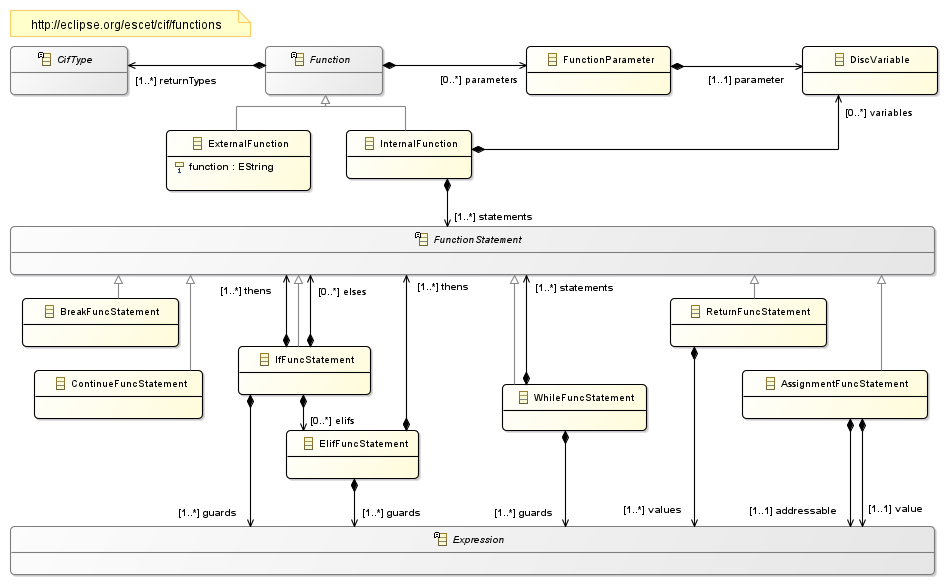
\includegraphics[width=\textwidth]{../model/images/functions.png}
  \caption{\textit{functions} package}\label{fig:pkg:functions}
\end{figure}

Figure~\ref{fig:pkg:functions} shows the \textit{functions} package.
The \cifclass{Function} class acts as a base class for all user-defined
functions. We have two concrete variants of user-defined functions: internal
user-defined functions, which are fully defined within the CIF specification,
and external user-defined function, for which the header is defined in the
CIF specification, and the actual implementation resides outside of the CIF
specification. The upper part of the diagram is mostly concerned with the
features common to all user-defined functions. The lower part contains the
statements that can be used in the internal user-defined functions.
}

% AssignmentFuncStatement (class)
\newcommand{\clsdocuAssignmentFuncStatement}{
An assignment internal function statement.

\begin{constraints}
\citem{AssignmentFuncStatement.types}
  The type of the assigned value must match the type of the addressable that is
  assigned. For ranged types, if the variable being assigned has a ranged
  type with a range, then the range of the type of the value must have
  overlap with the range of the type of the variable. It is considered a
  run-time error if the evaluated value expression results in a value that
  is outside of the range of the assigned variable.
\end{constraints}
}

\newcommand{\featdocuAssignmentFuncStatementaddressable}{
The addressable (a variable, a part of a variable, multiple variables, parts
of multiple variables, etc) to which to assign a value.

It is allowed to create a new key/value pair in a dictionary, if the key of the
last projection does not exist. It is not allowed to create a new key/value
pair, if the key of one of the other projections does not exist.

\begin{constraints}
\citem{AssignmentFuncStatement.addressableSyntax}
  Addressables may be discrete variable references (non-wrapped), with
  projections, and may optionally be wrapped in tuples (possibly multiple
  times). Projected string typed variables are not allowed.
\citem{AssignmentFuncStatement.variablesInScope}
  The variables that are assigned must be local variables declared in the
  same function as the assignment statement, or they must be parameters of that
  same function. Local variables and parameters may be mixed in a single
  assignment.
\citem{AssignmentFuncStatement.uniqueVariables}
  The parts of variables that are assigned must be unique. That is, it must
  never be possible to assign the same part of the same variable twice. We do
  include the projections in the analysis, but only as far as we can statically
  evaluate and normalize the indices. See the `Edge.uniqueVariables' constraint
  for the complete details.
\end{constraints}
}

\newcommand{\featdocuAssignmentFuncStatementvalue}{
The value to assign to the variables.
}

% BreakFuncStatement (class)
\newcommand{\clsdocuBreakFuncStatement}{
A break internal function statement. Breaks out of the closest enclosing
while statement.

\begin{constraints}
\citem{BreakFuncStatement.occurrence}
  Break statements may only occur in the body of while statements.
\end{constraints}
}

% ContinueFuncStatement (class)
\newcommand{\clsdocuContinueFuncStatement}{
A continue internal function statement. Continues with the next iteration
(if any) of the closest enclosing while statement, or breaks out of it
(if the guards no longer hold).

\begin{constraints}
\citem{ContinueFuncStatement.occurrence}
  Continue statements may only occur in the body of while statements.
\end{constraints}
}

% ElifFuncStatement (class)
\newcommand{\clsdocuElifFuncStatement}{
An `elif' (`else-if') alternative of an \cifclass{IfFuncStatement}.
}

\newcommand{\featdocuElifFuncStatementguards}{
The guard predicates for this alternative.

If multiple predicates are given, this feature represents the logical
conjunction of those predicates. Note that this represents the mathematical
conjunction, and not the short-circuit conjunction binary operator. As such,
there is no ordering between the guards.

\begin{constraints}
\citem{ElifFuncStatement.guardTypes}
  The guard predicates must have boolean types.
\end{constraints}
}

\newcommand{\featdocuElifFuncStatementthens}{
The statements to execute for the \cifclass{ElifFuncStatement} if the `guards'
evaluate to \emph{true}.
}

% ExternalFunction (class)
\newcommand{\clsdocuExternalFunction}{
An external user-defined function. The CIF specification only defines the
header of the function, and the actual implementation resides outside of the
CIF specification.

External user-defined functions are generally used to allow access from within
CIF specifications to algorithms and functions defined in other languages.
Functions are used to perform calculations, rather than for parts of the
system that have run-time behavior, such as discrete event control algorithms,
or hybrid dynamics.

\begin{constraints}
\citem{ExternalFunction.uniqueParams}
  The names of all parameters of the function, must be unique within that
  function.
\end{constraints}
}

\newcommand{\featdocuExternalFunctionfunction}{
A textual reference to the external implementation of the function. The
contents is interpreted by the tooling, such as for instance simulators.
}

% Function (abstract class)
\newcommand{\clsdocuFunction}{
Base class for all external user-defined functions.

We use value semantics for the parameters of functions.

\begin{constraints}
\citem{Function.sideEffectFree}
  All user-defined functions in CIF are pure mathematical functions and
  therefore, must be deterministic, and may not have side effects.

  This is enforced for internal user-defined functions by not allowing the use
  of variable `time', the scoping rules regarding references to objects outside
  of the function, and the restricted use of distribution standard library
  functions.

  For external user-defined functions, it is (often) impossible to check this
  constraint in an implementation, and the responsibility for checking this is
  therefore delegated to the end user. Practically, this means that for
  instance logging statements in functions, while essentially side effects, may
  be permitted, as long as the function returns the same value, if given the
  same arguments. This is essential for correct simulation results, as the
  results of function calls may for instance be cached by a simulator.
\end{constraints}

% Unique name constraints in derived classes.
}

\newcommand{\featdocuFunctionparameters}{
The parameters of the user-defined function.
}

\newcommand{\featdocuFunctionreturnTypes}{
The return types of the user-defined function. If multiple types are defined,
then the return type of the function is a tuple with nameless fields of those
types.

\begin{constraints}
\citem{Function.allowedReturnTypes}
  Component types and component definition types are not allowed in return
  types of functions, as components and component definitions are not meant to
  be used as values.
\end{constraints}
}

% FunctionParameter (class)
\newcommand{\clsdocuFunctionParameter}{
A parameter of a user-defined function.
}

\newcommand{\featdocuFunctionParameterparameter}{
The discrete variable, doubling as the function parameter. Reusing the
\cifclass{DiscVariable} class makes it possible to use the same references
as for discrete variables, also for function parameters.

\begin{constraints}
\citem{FunctionParameter.allowedTypes}
  Component types and component definition types are not allowed for function
  parameters, as components and component definitions are not meant to be used
  as values.
\citem{FunctionParameter.noValue}
  The \emph{parameter} declaration must not have a value, since the function
  argument should provide it.
\end{constraints}
}

% FunctionStatement (abstract class)
\newcommand{\clsdocuFunctionStatement}{
Base class for all statements of internal user-defined functions.
}

% IfFuncStatement (class)
\newcommand{\clsdocuIfFuncStatement}{
A conditional internal function statement.
}

\newcommand{\featdocuIfFuncStatementelifs}{
The `else-if' (`elif') alternatives. Processed in order, if the `guards'
evaluate to \emph{false}.
}

\newcommand{\featdocuIfFuncStatementelses}{
The `else' statements. If present, these statements are executed if no other
alternative has a \emph{true} guard.
}

\newcommand{\featdocuIfFuncStatementguards}{
The guard predicates for the `then' statements.

If multiple predicates are given, this feature represents the logical
conjunction of those predicates. Note that this represents the mathematical
conjunction, and not the short-circuit conjunction binary operator. As such,
there is no ordering between the guards.

\begin{constraints}
\citem{IfFuncStatement.guardTypes}
  The guard predicates must have boolean types.
\end{constraints}
}

\newcommand{\featdocuIfFuncStatementthens}{
The `then' statements. Executed if the `guards' evaluate to \emph{true}.
}

% InternalFunction (class)
\newcommand{\clsdocuInternalFunction}{
An internal user-defined function. The function is completely defined within
the CIF specification.

\begin{constraints}
\citem{InternalFunction.uniqueDecls}
  The names of all parameters and local variables in the body of the function,
  must be unique within that function.
\citem{InternalFunction.endWithReturn}
  All executions/evaluations of the function must end with a return statement.
\citemnf{InternalFunction.unreachable}
  Unreachable statements are not allowed.
\end{constraints}
}

\newcommand{\featdocuInternalFunctionstatements}{
The statements that form the body of the internal user-defined function.
}

\newcommand{\featdocuInternalFunctionvariables}{
The local variable declarations of the internal user-defined function.
Reusing the \cifclass{DiscVariable} class makes it possible to use the same
references as for discrete variables, also for local variables of functions.

\begin{constraints}
\citem{InternalFunction.allowedVarTypes}
  Component types and component definition types are not allowed for local
  variables of functions, as components and component definitions are not
  meant to be used as values.
\citem{InternalFunction.deterministicVarInit}
  Local variables of functions must have at most one initial value. That is,
  they may not be initialized in a non-deterministic way. In other words,
  they are either given an explicit initial value, or they get the default
  value for their type. For the default values for each of the CIF types,
  see the \emph{value} feature of the \cifclass{DiscVariable} class.
\end{constraints}
}

% ReturnFuncStatement (class)
\newcommand{\clsdocuReturnFuncStatement}{
A return internal function statement.
}

\newcommand{\featdocuReturnFuncStatementvalues}{
The return values of the return statement.

\begin{constraints}
\citem{ReturnFuncStatement.types}
  The types of the return values must match the return types of the function.
  For ranged types, if a return type has a ranged type with a range, then
  the range of the type of the corresponding return value, must be entirely
  contained in the range of the return type.
\end{constraints}
}

% WhileFuncStatement (class)
\newcommand{\clsdocuWhileFuncStatement}{
A while internal function statement.
}

\newcommand{\featdocuWhileFuncStatementguards}{
The guard predicates for the `while' statements.

If multiple predicates are given, this feature represents the logical
conjunction of those predicates. Note that this represents the mathematical
conjunction, and not the short-circuit conjunction binary operator. As such,
there is no ordering between the guards.

\begin{constraints}
\citem{WhileFuncStatement.guardTypes}
  The guard predicates must have boolean types.
\end{constraints}
}

\newcommand{\featdocuWhileFuncStatementstatements}{
The statements that form the body of the while statement.
}


%%%%%%%%%%%%%%%%%%%%%%%%%%%%%%%%%%%%%%%%%%%%%%%%%%%%%%%%%%%%%%%%%%%%%%%%%%%%%%%
% Package cifsvg
%%%%%%%%%%%%%%%%%%%%%%%%%%%%%%%%%%%%%%%%%%%%%%%%%%%%%%%%%%%%%%%%%%%%%%%%%%%%%%%
\newcommand{\pkgdocucifsvg}{
\begin{figure}
  \centering
  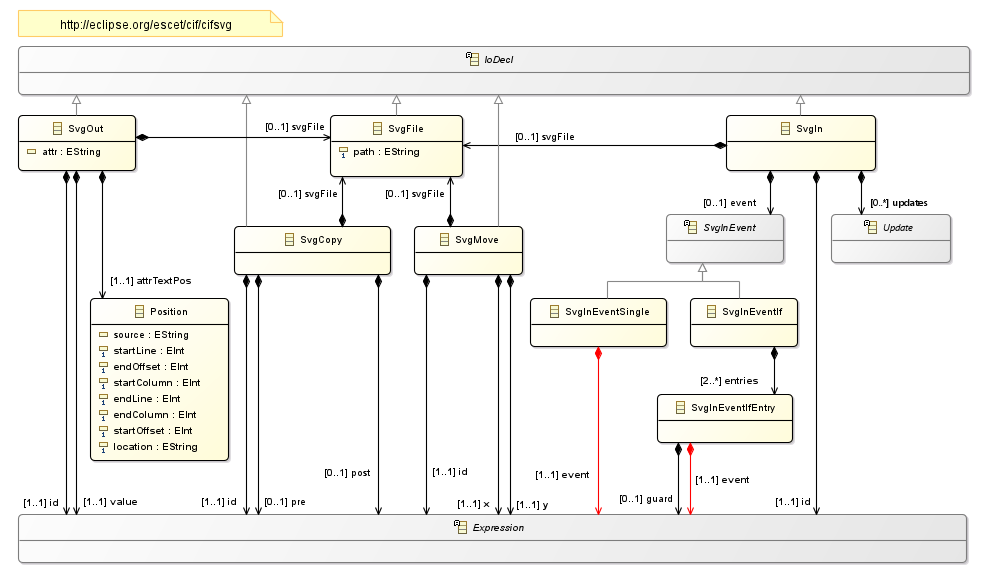
\includegraphics[width=\textwidth]{../model/images/cifsvg.png}
  \caption{\textit{cifsvg} package}\label{fig:pkg:cifsvg}
\end{figure}

Figure~\ref{fig:pkg:cifsvg} shows the \textit{cifsvg} package.
This package contains classes that describe CIF/SVG I/O declarations, used to
couple CIF models to SVG images, for SVG visualization. CIF/SVG I/O
declarations fall outside of the simulation behavior/semantics of the model.
The \cifclass{SvgFile} class declares the SVG file to use, the
other declarations specifies how to modify the SVG image during simulation, and
how to interact with it.
}

% SvgCopy (class)
\newcommand{\clsdocuSvgCopy}{
SVG copy declaration. Copies a part of the SVG tree, and renames the copied
elements.

\begin{constraints}
\citem{SvgCopy.svgFileDefined}
  Either the copy declaration specifies an SVG file to use, or one of the
  ancestors of the copy declaration does.
\citemnf{SvgCopy.overlap}
  The tree to copy must not be a subtree of any other tree that is copied, as
  the result is then dependent on the order of application of the copies.
  Copying the exact same tree (same root elements) multiple times however,
  does not pose any problems.
\citem{SvgCopy.unique}
  The ids of the elements in copied tree, after prefixing and/or postfixing
  them, should be unique in the SVG image.
\citem{SvgCopy.prePost}
  A prefix value or a postfix value must be specified, or both of them, but not
  neither of them.
\citem{SvgCopy.nonRoot}
  Copying the root element of an SVG image's XML tree is not allowed, as copies
  are added as siblings of their originals, and there can only be one root
  element.
\end{constraints}
}

\newcommand{\featdocuSvgCopyid}{
The `id' of the SVG element that is root of the tree to copy.

\begin{constraints}
\citem{SvgCopy.idType}
  The `id' expression must have a string type.
\citem{SvgCopy.idStaticEval}
  The expression must be statically evaluable, after elimination of component
  definition/instantiation, and checking for cycles. In particular, it must not
  change during simulation.
\citem{SvgCopy.idExists}
  An element with the given `id` must exist in the SVG image.
\citem{SvgCopy.idValidName}
  The `id' must be a valid XML/SVG name.
\end{constraints}
}

\newcommand{\featdocuSvgCopypost}{
The text to postfix to the names of copied SVG elements.

\begin{constraints}
\citem{SvgCopy.postType}
  The `post' expression must have a string type.
\citem{SvgCopy.postStaticEval}
  The expression must be statically evaluable, after elimination of component
  definition/instantiation, and checking for cycles. In particular, it must not
  change during simulation.
\citem{SvgCopy.postValidName}
  The `post' must be a valid XML/SVG name postfix.
\end{constraints}
}

\newcommand{\featdocuSvgCopypre}{
The text to prefix to the names of copied SVG elements.

\begin{constraints}
\citem{SvgCopy.preType}
  The `pre' expression must have a string type.
\citem{SvgCopy.preStaticEval}
  The expression must be statically evaluable, after elimination of component
  definition/instantiation, and checking for cycles. In particular, it must not
  change during simulation.
\citem{SvgCopy.preValidName}
  The `pre' must be a valid XML/SVG name prefix.
\end{constraints}
}

\newcommand{\featdocuSvgCopysvgFile}{
If specified, indicates the SVG image to use for the copy declaration. If not
specified, the SVG image specified by the closest ancestor that specifies an
SVG image is used.
}

% SvgFile (class)
\newcommand{\clsdocuSvgFile}{
A declaration of the SVG file to use for the CIF/SVG declarations. If specified
in a component, it applies to that component and all its children recursively,
unless overridden in a deeper scope or CIF/SVG declaration. If specified in
a CIF/SVG declaration, it applies only to that specific CIF/SVG declaration.

\begin{constraints}
\citem{SvgFile.validSvgFile}
  The SVG file must exist on disk, and be a valid SVG file.
\end{constraints}
}

\newcommand{\featdocuSvgFilepath}{
The absolute or relative local file system path to the SVG image to use. May
use both \texttt{/} and \texttt{\textbackslash} as file separators. If
relative, the path is relative to the path of the CIF file.
}

% SvgIn (class)
\newcommand{\clsdocuSvgIn}{
A CIF/SVG input mapping. Used to specify how clicking a certain element of the
SVG image influences the traces chosen by the CIF simulator. In other words,
it turns a certain element of the SVG image into an interactive SVG element.

\begin{constraints}
\citem{SvgIn.svgFileDefined}
  Either the input mapping specifies an SVG file to use, or one of the
  ancestors of the input mapping does.
\citem{SvgIn.unique}
  No two input mappings may be defined for the same element `id', per SVG file.
\citem{SvgIn.eventOrUpdate}
  Either the input mapping specifies which event to choose during simulation or
  which updates to execute during simulation.
\end{constraints}
}

\newcommand{\featdocuSvgInid}{
The `id' of the interactive SVG element.

\begin{constraints}
\citem{SvgIn.idType}
  The `id' expression must have a string type.
\citem{SvgIn.idStaticEval}
  The expression must be statically evaluable, after elimination of component
  definition/instantiation, and checking for cycles. In particular, it must not
  change during simulation.
\citem{SvgIn.idExists}
  An element with the given `id` must exist in the SVG image.
\citem{SvgIn.idValidName}
  The `id' must be a valid XML/SVG name.
\end{constraints}
}

\newcommand{\featdocuSvgInevent}{
A specification of which event to choose during simulation, when the
interactive SVG element for this input mapping is clicked.
}

\newcommand{\featdocuSvgInupdates}{
A specification of which updates to execute during simulation, when the
interactive SVG element for this input mapping is clicked.

\begin{constraints}
\citem{SvgIn.uniqueVariables}
  The parts of variables that are assigned must be unique. That is, it must
  never be possible to assign the same part of the same variable twice. We do
  include the projections in the analysis, but only as far as we can statically
  evaluate and normalize the indices. See the `Edge.uniqueVariables' constraint
  for the complete details.
\end{constraints}
}

\newcommand{\featdocuSvgInsvgFile}{
If specified, indicates the SVG image to use for the input mapping. If not
specified, the SVG image specified by the closest ancestor that specifies an
SVG image is used.
}

% SvgInEvent (abstract class)
\newcommand{\clsdocuSvgInEvent}{
A specification of the which event to choose during simulation, when an
interactive SVG element for an input mapping is clicked.
}

% SvgInEventIf (class)
\newcommand{\clsdocuSvgInEventIf}{
CIF/SVG input mapping event choice using an if/then/else construction.
}

\newcommand{\featdocuSvgInEventIfentries}{
The entries of the if/then/else. The first entry is the `if'. The remaining
entries are `elif' entries. If the last entry has no `guard', the entry
represents and `else'. The entries are evaluated in the given order.

It is considered a runtime error if none of the entries can be chosen at
runtime.

\begin{constraints}
\citem{SvgInEventIf.else}
  Only the last entry may be an `else', and may thus omit the `guard'.
\end{constraints}
}

% SvgInEventIfEntry (class)
\newcommand{\clsdocuSvgInEventIfEntry}{
A single entry of a CIF/SVG input mapping `if' event choice.
}

\newcommand{\featdocuSvgInEventIfEntryevent}{
The event to choose if the \emph{guard} holds.

This feature contains \cifclass{Expression} instances, to allow for wrapping
expressions to be used. See also Section~\ref{sec:scoping}.

\begin{constraints}
\citem{SvgInEventIfEntry.event}
  The event reference expression must refer to an event.
\citem{SvgInEventIfEntry.eventInScope}
  The event reference must satisfy the scoping rules.
\end{constraints}
}

\newcommand{\featdocuSvgInEventIfEntryguard}{
The guard predicates of the entry. The entry is only `chosen' if the guard
evaluates to \emph{true}.

If no predicate is given, the entry acts as an emph{else}, and can always
be chosen (essentially a \emph{true} guard).

\begin{constraints}
\citem{SvgInEventIfEntry.guardType}
  The guard predicate must have a boolean type.
\end{constraints}
}

% SvgInEventSingle (class)
\newcommand{\clsdocuSvgInEventSingle}{
CIF/SVG input mapping event choice that always chooses the same event.
}

\newcommand{\featdocuSvgInEventSingleevent}{
The event to choose.

This feature contains \cifclass{Expression} instances, to allow for wrapping
expressions to be used. See also Section~\ref{sec:scoping}.

\begin{constraints}
\citem{SvgInEventSingle.event}
  The event reference expression must refer to an event.
\citem{SvgInEventSingle.eventInScope}
  The event reference must satisfy the scoping rules.
\end{constraints}
}

% SvgMove (class)
\newcommand{\clsdocuSvgMove}{
SVG move declaration. Moves a shape to an absolute position.

\begin{constraints}
\citem{SvgMove.svgFileDefined}
  Either the move declaration specifies an SVG file to use, or one of the
  ancestors of the move declaration does.
\citem{SvgMove.noTransform}
  If an SVG element is moved, it must not also have an SVG output mapping for
  the `transform' attribute, as that would override the move.
\citem{SvgMove.unique}
  No two move declarations may be defined for the same element `id', per SVG
  file.
\end{constraints}
}

\newcommand{\featdocuSvgMoveid}{
The `id' of the SVG element for which the shape is to be moved.

\begin{constraints}
\citem{SvgMove.idType}
  The `id' expression must have a string type.
\citem{SvgMove.idStaticEval}
  The expression must be statically evaluable, after elimination of component
  definition/instantiation, and checking for cycles. In particular, it must not
  change during simulation.
\citem{SvgMove.idExists}
  An element with the given `id` must exist in the SVG image.
\citem{SvgMove.idValidName}
  The `id' must be a valid XML/SVG name.
\end{constraints}
}

\newcommand{\featdocuSvgMovesvgFile}{
If specified, indicates the SVG image to use for the move declaration. If not
specified, the SVG image specified by the closest ancestor that specifies an
SVG image is used.
}

\newcommand{\featdocuSvgMovex}{
The x coordinate of the upper left corner of the bounding box of the shape to
move, relative to the upper left corner of the canvas, after moving.

\begin{constraints}
\citem{SvgMove.xType}
  The `x' expression must have an numeric (integer or real) type.
\citem{SvgMove.xStaticEval}
  The expression must be statically evaluable, after elimination of component
  definition/instantiation, and checking for cycles. In particular, it must not
  change during simulation.
\end{constraints}
}

\newcommand{\featdocuSvgMovey}{
The y coordinate of the upper left corner of the bounding box of the shape to
move, relative to the upper left corner of the canvas, after moving.

\begin{constraints}
\citem{SvgMove.yType}
  The `y' expression must have an numeric (integer or real) type.
\citem{SvgMove.yStaticEval}
  The expression must be statically evaluable, after elimination of component
  definition/instantiation, and checking for cycles. In particular, it must not
  change during simulation.
\end{constraints}
}

% SvgOut (class)
\newcommand{\clsdocuSvgOut}{
A CIF/SVG output mapping. Used to specify how the state of the CIF model is to
be used to update the SVG image, during simulation.

\begin{constraints}
\citem{SvgOut.svgFileDefined}
  Either the output mapping specifies an SVG file to use, or one of the
  ancestors of the output mapping does.
\citem{SvgOut.unique}
  No two output mappings may be defined for the same element `id' and attribute
  name, per SVG file. Similarly, no two output mappings may be defined for the
  same text node (taking into account that different element ids may lead to
  the same text node), per SVG file.
\end{constraints}
}

\newcommand{\featdocuSvgOutattr}{
If specified, indicates the name of the attribute of which to change the value.
If not specified, indicates that the text of the element is to be changed.

\begin{constraints}
\citem{SvgOut.textNode}
  If no attribute name is specified, the SVG element must have a text node.
\citem{SvgOut.attrValidName}
  If an attribute name is specified, it must be a valid XML/SVG name.
\citemnf{SvgOut.elemNameInSvg11}
  If an attribute name is specified, the name of the element (not its `id'),
  must be defined in the SVG 1.1 standard.
\citemnf{SvgOut.attrNameInSvg11}
  If an attribute name is specified, the attribute name must be defined for
  the element, in the SVG 1.1 standard.
\citem{SvgOut.attrId}
  If an attribute name is specified, it must not be the \texttt{id}
  attribute, in any casing.
\citem{SvgOut.attrStyle}
  If an attribute name is specified, it must not be the \texttt{style}
  attribute, in any casing.
\end{constraints}
}

\newcommand{\featdocuSvgOutattrTextPos}{
Position information for the attribute string literal of the output mapping, or
for the \texttt{text} keyword of the output mapping.
}

\newcommand{\featdocuSvgOutid}{
The `id' of the SVG element to modify.

\begin{constraints}
\citem{SvgOut.idType}
  The `id' expression must have a string type.
\citem{SvgOut.idStaticEval}
  The expression must be statically evaluable, after elimination of component
  definition/instantiation, and checking for cycles. In particular, it must not
  change during simulation.
\citem{SvgOut.idExists}
  An element with the given `id` must exist in the SVG image.
\citem{SvgOut.idValidName}
  The `id' must be a valid XML/SVG name.
\end{constraints}
}

\newcommand{\featdocuSvgOutsvgFile}{
If specified, indicates the SVG image to use for the output mapping. If not
specified, the SVG image specified by the closest ancestor that specifies an
SVG image is used.
}

\newcommand{\featdocuSvgOutvalue}{
The expression to evaluate to obtain the value to use as output, to set the
value of the attribute or text label.

\begin{constraints}
\citem{SvgOut.valueType}
  Component types and component definition types are not allowed for the value,
  as components and component definitions are not meant to be used as values.
\end{constraints}
}


%%%%%%%%%%%%%%%%%%%%%%%%%%%%%%%%%%%%%%%%%%%%%%%%%%%%%%%%%%%%%%%%%%%%%%%%%%%%%%%
% Package print
%%%%%%%%%%%%%%%%%%%%%%%%%%%%%%%%%%%%%%%%%%%%%%%%%%%%%%%%%%%%%%%%%%%%%%%%%%%%%%%
\newcommand{\pkgdocuprint}{
\begin{figure}
  \centering
  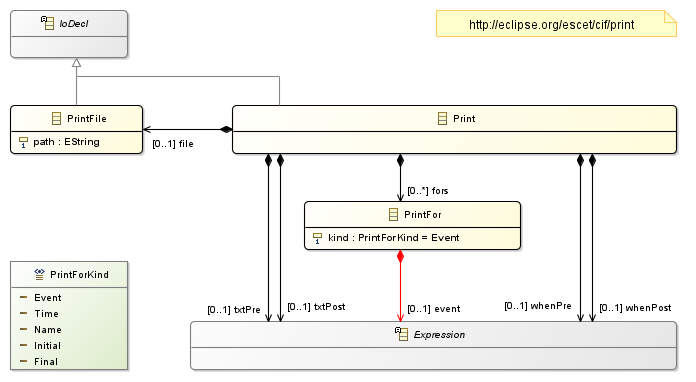
\includegraphics[width=\textwidth]{../model/images/print.png}
  \caption{\textit{print} package}\label{fig:pkg:print}
\end{figure}

Figure~\ref{fig:pkg:print} shows the \textit{print} package.
This package contains classes that describe print I/O declarations, used to
produce textual output from CIF models. Print I/O declarations fall outside of
the simulation behavior/semantics of the model. The \cifclass{PrintFile} class
declares the file (or target) to which to print the text, while the
\cifclass{Print} class specifies what to print and when to print it.
}

% PrintForKind (enumeration)
\newcommand{\enumdocuPrintForKind}{
Specifies the kind of a 'for' filter of a \cifclass{PrintFor} class.
}

\newcommand{\enumlitdocuPrintForKindEvent}{
Filter that includes all event transitions.
}

\newcommand{\enumlitdocuPrintForKindFinal}{
Filter that includes the virtual transition after the last (final or deadlock)
state.
}

\newcommand{\enumlitdocuPrintForKindInitial}{
Filter that includes the virtual transition before the first (initial) state.
}

\newcommand{\enumlitdocuPrintForKindName}{
Filter that includes the event transitions for a specific event.
}

\newcommand{\enumlitdocuPrintForKindTime}{
Filter that includes all time transitions.
}

% Print (class)
\newcommand{\clsdocuPrint}{
Print I/O declaration. Specifies what to print and when to print it.

\begin{constraints}
\citem{Print.txtPrePost}
  A pre/source or post/target state text must be specified, or both of them,
  but not neither of them.
\end{constraints}
}

\newcommand{\featdocuPrintfile}{
The file (or target) to which to print the text.

If not specified, the file specified by the closest ancestor that specifies a
\cifclass{PrintFile} is used. If none exists, \texttt{":stdout"} is used.
}

\newcommand{\featdocuPrintfors}{
The `for' filters for this print declaration. Only transitions for which at
least one of the filters matches, lead to text being printed. If no filters
are specified, it defaults to \texttt{initial, event, time}.

\begin{constraints}
\citemnf{Print.duplFor}
  The `for' filters should not contain duplicates (be overspecified). That is,
  specifying the same kind multiple times should be avoided (except
  \cifenumlit{PrintForKind.Name}). Furthermore, specifying the same event
  multiple times should be avoided. Finally, specifying
  \cifenumlit{PrintForKind.Event} (all events) and
  \cifenumlit{PrintForKind.Name} (specific event) should be avoided.
\end{constraints}
}

\newcommand{\featdocuPrinttxtPost}{
If specified, indicates the text to print for the post/target state.

Evaluation result is converted to a textual representation. String typed
results are a special case, as no double quotes are added, and escaping is not
performed.

\begin{constraints}
\citemnf{Print.txtPostType}
  The type of a print declaration post text, if specified, must not have a
  component or component definition type.
\end{constraints}
}

\newcommand{\featdocuPrinttxtPre}{
If specified, indicates the text to print for the pre/source state.

Evaluation result is converted to a textual representation. String typed
results are a special case, as no double quotes are added, and escaping is not
performed.

\begin{constraints}
\citemnf{Print.txtPreType}
  The type of a print declaration pre text, if specified, must not have a
  component or component definition type.
\end{constraints}
}

\newcommand{\featdocuPrintwhenPost}{
If specified, filters post/target states. Text is only printed if the predicate
holds for a post/target state.

\begin{constraints}
\citem{Print.whenPostType}
  The `when` `post` predicate must have a boolean type.
\end{constraints}
}

\newcommand{\featdocuPrintwhenPre}{
If specified, filters pre/source states. Text is only printed if the predicate
holds for a pre/source state.

\begin{constraints}
\citem{Print.whenPreType}
  The `when' `pre' predicate must have a boolean type.
\end{constraints}
}

% PrintFile (class)
\newcommand{\clsdocuPrintFile}{
The file (or target) to which to print text. Applies to the scope in which it
is specified, and all child scopes recursively, unless overridden in a deeper
scope.
}

\newcommand{\featdocuPrintFilepath}{
The path of file (or target). If it refers to a file, it must be an absolute
or relative local file system path to the file. May use both \texttt{/} and
\texttt{\textbackslash} as file separators. If relative, the path is relative
to the path of the CIF file. Special values, such as \texttt{":stdout"}, are
supported as well.
}

% PrintFor (class)
\newcommand{\clsdocuPrintFor}{
A `for' filter of a \cifclass{Print}. Filters transitions to keep only those
that match the `for' filter.

\begin{constraints}
\citem{PrintFor.eventSpecified}
  The `event' must be specified if and only if the `kind' is
  \cifenumlit{PrintForKind.Name}.
\end{constraints}
}

\newcommand{\featdocuPrintForevent}{
The event to include, for this `for' filter.

This feature contains \cifclass{Expression} instances, to allow for wrapping
expressions to be used. See also Section~\ref{sec:scoping}.

\begin{constraints}
\citem{PrintFor.event}
  The event reference expression must refer to an event.
\citem{PrintFor.eventInScope}
  The event reference must satisfy the scoping rules.
\end{constraints}
}

\newcommand{\featdocuPrintForkind}{
The kind of the `for' filter.
}


%%%%%%%%%%%%%%%%%%%%%%%%%%%%%%%%%%%%%%%%%%%%%%%%%%%%%%%%%%%%%%%%%%%%%%%%%%%%%%%
% Package annotations
%%%%%%%%%%%%%%%%%%%%%%%%%%%%%%%%%%%%%%%%%%%%%%%%%%%%%%%%%%%%%%%%%%%%%%%%%%%%%%%
\newcommand{\pkgdocuannotations}{
\begin{figure}
  \centering
  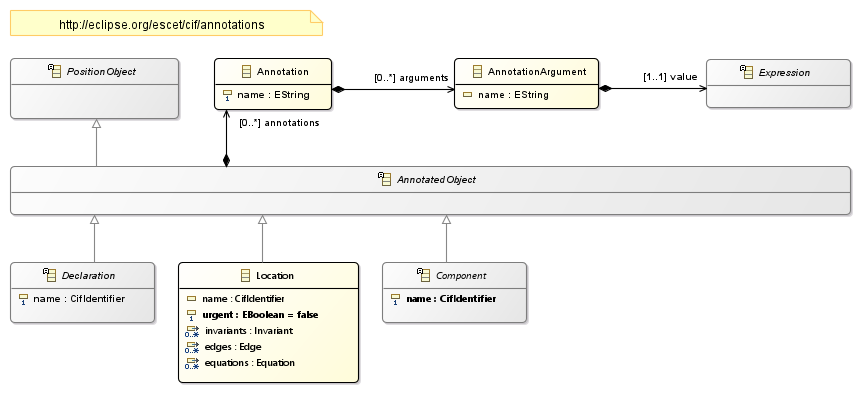
\includegraphics[width=\textwidth]{../model/images/annotations.png}
  \caption{\textit{annotations} package}\label{fig:pkg:annotations}
\end{figure}

Figure~\ref{fig:pkg:annotations} shows the \textit{annotations} package.
The main class is the \cifclass{Annotation} class. It represents a single
annotations on a single object. The \cifclass{AnnotationArgument} class
represents a single arguments of an annotation. And the
\cifclass{AnnotatedObject} class is the base class for all objects
that can be annotated.
}

% AnnotatedObject (abstract class)
\newcommand{\clsdocuAnnotatedObject}{
Base class for all objects that can be annotated.
}

\newcommand{\featdocuAnnotatedObjectannotations}{
The annotations of the annotated object.

\begin{constraints}
\citem{AnnotatedObject.onlyForSupportedObjects}
  Currently only the following objects support annotations:
  \begin{itemize}
    \item Algebraic variables.
    \item Constants.
    \item Continuous variables.
    \item Discrete variables. But not parameters and local variables of internal user-defined functions.
    \item Events.
    \item Input variables.
    \item Locations of automata.
  \end{itemize}
\end{constraints}
}

% Annotation (class)
\newcommand{\clsdocuAnnotation}{
An annotation.

\begin{constraints}
\citem{Annotation.annotationSpecificErrors}
  The annotation and its arguments must satisfy any additional constraints
  imposed on the annotation by the registered annotation provider.
\citemnf{Annotation.annotationSpecificWarnings}
  The annotation and its arguments must satisfy any additional constraints
  imposed on the annotation by the registered annotation provider.
\end{constraints}
}

\newcommand{\featdocuAnnotationarguments}{
The arguments of the annotation.

\begin{constraints}
\citem{Annotation.uniqueArguments}
  The names of each of the arguments must be unique within the annotation.
\end{constraints}
}

\newcommand{\featdocuAnnotationname}{
The name of the annotation.

\begin{constraints}
\citem{Annotation.validName}
  The name must be a CIF identifier, or multiple CIF identifiers joined
  together using colons (\texttt{:}). For instance, \texttt{name} or
  \texttt{some:name}.
\citemnf{Annotation.registeredName}
  The annotation name must be a registered annotation name, within the
  environment where the CIF model is used.
\end{constraints}
}

% AnnotationArgument (class)
\newcommand{\clsdocuAnnotationArgument}{
An argument of an \cifclass{Annotation}.
}

\newcommand{\featdocuAnnotationArgumentname}{
The name of the annotation argument.

\begin{constraints}
\citem{AnnotationArgument.validName}
  The name must be a CIF identifier, or multiple CIF identifiers joined
  together using periods (\texttt{.}). For instance, \texttt{arg} or
  \texttt{some.arg}.
\end{constraints}
}

\newcommand{\featdocuAnnotationArgumentvalue}{
The value of the annotation argument.
}

%%%%%%%%%%%%%%%%%%%%%%%%%%%%%%%%%%%%%%%%%%%%%%%%%%%%%%%%%%%%%%%%%%%%%%%%%%%%%%%
%% Copyright (c) 2010, 2023 Contributors to the Eclipse Foundation
%%
%% See the NOTICE file(s) distributed with this work for additional
%% information regarding copyright ownership.
%%
%% This program and the accompanying materials are made available under the terms
%% of the MIT License which is available at https://opensource.org/licenses/MIT
%%
%% SPDX-License-Identifier: MIT
%%%%%%%%%%%%%%%%%%%%%%%%%%%%%%%%%%%%%%%%%%%%%%%%%%%%%%%%%%%%%%%%%%%%%%%%%%%%%%%

%\newcommand{\cifpkg}[1]{\textit{#1} (Section~\ref{cifpkg:#1})}
%\newcommand{\cifclass}[1]{\textit{#1} (Section~\ref{cifclass:#1})}
%\newcommand{\cifattr}[1]{\textit{#1} (Section~\ref{cifattr:#1})}
%\newcommand{\cifenumlit}[1]{\textit{#1} (Section~\ref{cifenumlit:#1})}
%\newcommand{\cifclassDetail}[7]{\item {#1} \textbf{#2} {#3} :
%    {\textit{#4}} {#5} {#6} \hfill \\ {#7}}
%\newcommand{\cifenumlitDetail}[4]{\item literal \textbf{#1} {#2} {#3}
%    \hfill \\ {#4}}
%\newcommand{\hook}{\hspace*{5pt}\raisebox{2.5pt}{$\llcorner$}}
%\newcommand{\hookindent}{\hspace*{15pt}}

\section{Package cif}\label{cifpkg:cif}
\pkgdocucif

\begin{description}
\item[Package URI] http://eclipse.org/escet/cif
\item[Namespace prefix] cif
\item[Sub-packages] \cifpkg{declarations}, \cifpkg{automata}, \cifpkg{types}, \cifpkg{expressions}, \cifpkg{functions}, \cifpkg{cifsvg}, \cifpkg{print}, \cifpkg{annotations}
\end{description}

\subsection{CifIdentifier (datatype)}\label{cifclass:CifIdentifier}
\dtypedocuCifIdentifier

\begin{description}
\item[Name] CifIdentifier
\item[Instance class name] java.lang.String
\item[Basetype] http://www.eclipse.org/emf/2002/Ecore\#EString
\item[Pattern] \verb@[A-Za-z_][A-Za-z0-9_]*@
\end{description}

\subsection{InvKind (enumeration)}\label{cifclass:InvKind}
\enumdocuInvKind

\begin{description}
\cifenumlitDetail{EventDisables}{}{\label{cifenumlit:InvKind.EventDisables}}{\enumlitdocuInvKindEventDisables}
\cifenumlitDetail{EventNeeds}{}{\label{cifenumlit:InvKind.EventNeeds}}{\enumlitdocuInvKindEventNeeds}
\cifenumlitDetail{State}{(default)}{\label{cifenumlit:InvKind.State}}{\enumlitdocuInvKindState}
\end{description}

\subsection{SupKind (enumeration)}\label{cifclass:SupKind}
\enumdocuSupKind

\begin{description}
\cifenumlitDetail{None}{(default)}{\label{cifenumlit:SupKind.None}}{\enumlitdocuSupKindNone}
\cifenumlitDetail{Plant}{}{\label{cifenumlit:SupKind.Plant}}{\enumlitdocuSupKindPlant}
\cifenumlitDetail{Requirement}{}{\label{cifenumlit:SupKind.Requirement}}{\enumlitdocuSupKindRequirement}
\cifenumlitDetail{Supervisor}{}{\label{cifenumlit:SupKind.Supervisor}}{\enumlitdocuSupKindSupervisor}
\end{description}

\subsection{AlgParameter (class)}\label{cifclass:AlgParameter}
\clsdocuAlgParameter

~\\ \noindent \emph{EObject} \\
\hook~\positionclass{PositionObject} \\
\hookindent\hook~\cifclass{Parameter} \\
\hookindent\hookindent\hook~\emph{AlgParameter}

~\\ \noindent Direct derived classes:
none

\begin{description}
\positionclassDetail{cont}{position}{{[0..1]}}{Position}{(inherited from \textit{PositionObject})}{\label{positionattr:AlgParameter.position}}
{\featdocuPositionObjectposition}
\cifclassDetail{cont}{variable}{{[1]}}{AlgVariable}{}{\label{cifattr:AlgParameter.variable}}
{\featdocuAlgParametervariable}
\end{description}


\subsection{ComplexComponent (abstract class)}\label{cifclass:ComplexComponent}
\clsdocuComplexComponent

~\\ \noindent \emph{EObject} \\
\hook~\positionclass{PositionObject} \\
\hookindent\hook~\cifclass{Component} \\
\hookindent\hookindent\hook~\emph{ComplexComponent}

~\\ \noindent Direct derived classes:
\cifclass{Automaton}, \cifclass{Group}

\begin{description}
\positionclassDetail{cont}{position}{{[0..1]}}{Position}{(inherited from \textit{PositionObject})}{\label{positionattr:ComplexComponent.position}}
{\featdocuPositionObjectposition}
\cifclassDetail{attr}{name}{{[1]}}{CifIdentifier}{(inherited from \textit{Component})}{\label{cifattr:ComplexComponent.name}}
{\featdocuComponentname}
\cifclassDetail{cont}{declarations}{{[0..*]}}{Declaration}{}{\label{cifattr:ComplexComponent.declarations}}
{\featdocuComplexComponentdeclarations}
\cifclassDetail{cont}{equations}{{[0..*]}}{Equation}{}{\label{cifattr:ComplexComponent.equations}}
{\featdocuComplexComponentequations}
\cifclassDetail{cont}{initials}{{[0..*]}}{Expression}{}{\label{cifattr:ComplexComponent.initials}}
{\featdocuComplexComponentinitials}
\cifclassDetail{cont}{invariants}{{[0..*]}}{Invariant}{}{\label{cifattr:ComplexComponent.invariants}}
{\featdocuComplexComponentinvariants}
\cifclassDetail{cont}{ioDecls}{{[0..*]}}{IoDecl}{}{\label{cifattr:ComplexComponent.ioDecls}}
{\featdocuComplexComponentioDecls}
\cifclassDetail{cont}{markeds}{{[0..*]}}{Expression}{}{\label{cifattr:ComplexComponent.markeds}}
{\featdocuComplexComponentmarkeds}
\end{description}


\subsection{Component (abstract class)}\label{cifclass:Component}
\clsdocuComponent

~\\ \noindent \emph{EObject} \\
\hook~\positionclass{PositionObject} \\
\hookindent\hook~\emph{Component}

~\\ \noindent Direct derived classes:
\cifclass{ComplexComponent}, \cifclass{ComponentInst}

\begin{description}
\positionclassDetail{cont}{position}{{[0..1]}}{Position}{(inherited from \textit{PositionObject})}{\label{positionattr:Component.position}}
{\featdocuPositionObjectposition}
\cifclassDetail{attr}{name}{{[1]}}{CifIdentifier}{}{\label{cifattr:Component.name}}
{\featdocuComponentname}
\end{description}


\subsection{ComponentDef (class)}\label{cifclass:ComponentDef}
\clsdocuComponentDef

~\\ \noindent \emph{EObject} \\
\hook~\positionclass{PositionObject} \\
\hookindent\hook~\emph{ComponentDef}

~\\ \noindent Direct derived classes:
none

\begin{description}
\positionclassDetail{cont}{position}{{[0..1]}}{Position}{(inherited from \textit{PositionObject})}{\label{positionattr:ComponentDef.position}}
{\featdocuPositionObjectposition}
\cifclassDetail{cont}{body}{{[1]}}{ComplexComponent}{}{\label{cifattr:ComponentDef.body}}
{\featdocuComponentDefbody}
\cifclassDetail{cont}{parameters}{{[0..*]}}{Parameter}{}{\label{cifattr:ComponentDef.parameters}}
{\featdocuComponentDefparameters}
\end{description}


\subsection{ComponentInst (class)}\label{cifclass:ComponentInst}
\clsdocuComponentInst

~\\ \noindent \emph{EObject} \\
\hook~\positionclass{PositionObject} \\
\hookindent\hook~\cifclass{Component} \\
\hookindent\hookindent\hook~\emph{ComponentInst}

~\\ \noindent Direct derived classes:
none

\begin{description}
\positionclassDetail{cont}{position}{{[0..1]}}{Position}{(inherited from \textit{PositionObject})}{\label{positionattr:ComponentInst.position}}
{\featdocuPositionObjectposition}
\cifclassDetail{attr}{name}{{[1]}}{CifIdentifier}{(inherited from \textit{Component})}{\label{cifattr:ComponentInst.name}}
{\featdocuComponentname}
\cifclassDetail{cont}{arguments}{{[0..*]}}{Expression}{}{\label{cifattr:ComponentInst.arguments}}
{\featdocuComponentInstarguments}
\cifclassDetail{cont}{definition}{{[1]}}{CifType}{}{\label{cifattr:ComponentInst.definition}}
{\featdocuComponentInstdefinition}
\end{description}


\subsection{ComponentParameter (class)}\label{cifclass:ComponentParameter}
\clsdocuComponentParameter

~\\ \noindent \emph{EObject} \\
\hook~\positionclass{PositionObject} \\
\hookindent\hook~\cifclass{Parameter} \\
\hookindent\hookindent\hook~\emph{ComponentParameter}

~\\ \noindent Direct derived classes:
none

\begin{description}
\positionclassDetail{cont}{position}{{[0..1]}}{Position}{(inherited from \textit{PositionObject})}{\label{positionattr:ComponentParameter.position}}
{\featdocuPositionObjectposition}
\cifclassDetail{attr}{name}{{[1]}}{CifIdentifier}{}{\label{cifattr:ComponentParameter.name}}
{\featdocuComponentParametername}
\cifclassDetail{cont}{type}{{[1]}}{CifType}{}{\label{cifattr:ComponentParameter.type}}
{\featdocuComponentParametertype}
\end{description}


\subsection{Equation (class)}\label{cifclass:Equation}
\clsdocuEquation

~\\ \noindent \emph{EObject} \\
\hook~\positionclass{PositionObject} \\
\hookindent\hook~\emph{Equation}

~\\ \noindent Direct derived classes:
none

\begin{description}
\positionclassDetail{cont}{position}{{[0..1]}}{Position}{(inherited from \textit{PositionObject})}{\label{positionattr:Equation.position}}
{\featdocuPositionObjectposition}
\cifclassDetail{attr}{derivative}{{[1]}}{EBoolean}{}{\label{cifattr:Equation.derivative}}
{\featdocuEquationderivative}
\cifclassDetail{cont}{value}{{[1]}}{Expression}{}{\label{cifattr:Equation.value}}
{\featdocuEquationvalue}
\cifclassDetail{ref}{variable}{{[1]}}{Declaration}{}{\label{cifattr:Equation.variable}}
{\featdocuEquationvariable}
\end{description}


\subsection{EventParameter (class)}\label{cifclass:EventParameter}
\clsdocuEventParameter

~\\ \noindent \emph{EObject} \\
\hook~\positionclass{PositionObject} \\
\hookindent\hook~\cifclass{Parameter} \\
\hookindent\hookindent\hook~\emph{EventParameter}

~\\ \noindent Direct derived classes:
none

\begin{description}
\positionclassDetail{cont}{position}{{[0..1]}}{Position}{(inherited from \textit{PositionObject})}{\label{positionattr:EventParameter.position}}
{\featdocuPositionObjectposition}
\cifclassDetail{cont}{event}{{[1]}}{Event}{}{\label{cifattr:EventParameter.event}}
{\featdocuEventParameterevent}
\cifclassDetail{attr}{recvFlag}{{[1]}}{EBoolean}{}{\label{cifattr:EventParameter.recvFlag}}
{\featdocuEventParameterrecvFlag}
\cifclassDetail{attr}{sendFlag}{{[1]}}{EBoolean}{}{\label{cifattr:EventParameter.sendFlag}}
{\featdocuEventParametersendFlag}
\cifclassDetail{attr}{syncFlag}{{[1]}}{EBoolean}{}{\label{cifattr:EventParameter.syncFlag}}
{\featdocuEventParametersyncFlag}
\end{description}


\subsection{Group (class)}\label{cifclass:Group}
\clsdocuGroup

~\\ \noindent \emph{EObject} \\
\hook~\positionclass{PositionObject} \\
\hookindent\hook~\cifclass{Component} \\
\hookindent\hookindent\hook~\cifclass{ComplexComponent} \\
\hookindent\hookindent\hookindent\hook~\emph{Group}

~\\ \noindent Direct derived classes:
\cifclass{Specification}

\begin{description}
\positionclassDetail{cont}{position}{{[0..1]}}{Position}{(inherited from \textit{PositionObject})}{\label{positionattr:Group.position}}
{\featdocuPositionObjectposition}
\cifclassDetail{attr}{name}{{[1]}}{CifIdentifier}{(inherited from \textit{Component})}{\label{cifattr:Group.name}}
{\featdocuComponentname}
\cifclassDetail{cont}{declarations}{{[0..*]}}{Declaration}{(inherited from \textit{ComplexComponent})}{\label{cifattr:Group.declarations}}
{\featdocuComplexComponentdeclarations}
\cifclassDetail{cont}{equations}{{[0..*]}}{Equation}{(inherited from \textit{ComplexComponent})}{\label{cifattr:Group.equations}}
{\featdocuComplexComponentequations}
\cifclassDetail{cont}{initials}{{[0..*]}}{Expression}{(inherited from \textit{ComplexComponent})}{\label{cifattr:Group.initials}}
{\featdocuComplexComponentinitials}
\cifclassDetail{cont}{invariants}{{[0..*]}}{Invariant}{(inherited from \textit{ComplexComponent})}{\label{cifattr:Group.invariants}}
{\featdocuComplexComponentinvariants}
\cifclassDetail{cont}{ioDecls}{{[0..*]}}{IoDecl}{(inherited from \textit{ComplexComponent})}{\label{cifattr:Group.ioDecls}}
{\featdocuComplexComponentioDecls}
\cifclassDetail{cont}{markeds}{{[0..*]}}{Expression}{(inherited from \textit{ComplexComponent})}{\label{cifattr:Group.markeds}}
{\featdocuComplexComponentmarkeds}
\cifclassDetail{cont}{components}{{[0..*]}}{Component}{}{\label{cifattr:Group.components}}
{\featdocuGroupcomponents}
\cifclassDetail{cont}{definitions}{{[0..*]}}{ComponentDef}{}{\label{cifattr:Group.definitions}}
{\featdocuGroupdefinitions}
\end{description}


\subsection{Invariant (class)}\label{cifclass:Invariant}
\clsdocuInvariant

~\\ \noindent \emph{EObject} \\
\hook~\positionclass{PositionObject} \\
\hookindent\hook~\emph{Invariant}

~\\ \noindent Direct derived classes:
none

\begin{description}
\positionclassDetail{cont}{position}{{[0..1]}}{Position}{(inherited from \textit{PositionObject})}{\label{positionattr:Invariant.position}}
{\featdocuPositionObjectposition}
\cifclassDetail{cont}{event}{{[0..1]}}{Expression}{}{\label{cifattr:Invariant.event}}
{\featdocuInvariantevent}
\cifclassDetail{attr}{invKind}{{[1]}}{InvKind}{}{\label{cifattr:Invariant.invKind}}
{\featdocuInvariantinvKind}
\cifclassDetail{attr}{name}{{[0..1]}}{CifIdentifier}{}{\label{cifattr:Invariant.name}}
{\featdocuInvariantname}
\cifclassDetail{cont}{predicate}{{[1]}}{Expression}{}{\label{cifattr:Invariant.predicate}}
{\featdocuInvariantpredicate}
\cifclassDetail{attr}{supKind}{{[1]}}{SupKind}{}{\label{cifattr:Invariant.supKind}}
{\featdocuInvariantsupKind}
\end{description}


\subsection{IoDecl (abstract class)}\label{cifclass:IoDecl}
\clsdocuIoDecl

~\\ \noindent \emph{EObject} \\
\hook~\positionclass{PositionObject} \\
\hookindent\hook~\emph{IoDecl}

~\\ \noindent Direct derived classes:
\cifclass{Print}, \cifclass{PrintFile}, \cifclass{SvgCopy}, \cifclass{SvgFile}, \cifclass{SvgIn}, \cifclass{SvgMove}, \cifclass{SvgOut}

\begin{description}
\positionclassDetail{cont}{position}{{[0..1]}}{Position}{(inherited from \textit{PositionObject})}{\label{positionattr:IoDecl.position}}
{\featdocuPositionObjectposition}
\end{description}


\subsection{LocationParameter (class)}\label{cifclass:LocationParameter}
\clsdocuLocationParameter

~\\ \noindent \emph{EObject} \\
\hook~\positionclass{PositionObject} \\
\hookindent\hook~\cifclass{Parameter} \\
\hookindent\hookindent\hook~\emph{LocationParameter}

~\\ \noindent Direct derived classes:
none

\begin{description}
\positionclassDetail{cont}{position}{{[0..1]}}{Position}{(inherited from \textit{PositionObject})}{\label{positionattr:LocationParameter.position}}
{\featdocuPositionObjectposition}
\cifclassDetail{cont}{location}{{[1]}}{Location}{}{\label{cifattr:LocationParameter.location}}
{\featdocuLocationParameterlocation}
\end{description}


\subsection{Parameter (abstract class)}\label{cifclass:Parameter}
\clsdocuParameter

~\\ \noindent \emph{EObject} \\
\hook~\positionclass{PositionObject} \\
\hookindent\hook~\emph{Parameter}

~\\ \noindent Direct derived classes:
\cifclass{AlgParameter}, \cifclass{ComponentParameter}, \cifclass{EventParameter}, \cifclass{LocationParameter}

\begin{description}
\positionclassDetail{cont}{position}{{[0..1]}}{Position}{(inherited from \textit{PositionObject})}{\label{positionattr:Parameter.position}}
{\featdocuPositionObjectposition}
\end{description}


\subsection{Specification (class)}\label{cifclass:Specification}
\clsdocuSpecification

~\\ \noindent \emph{EObject} \\
\hook~\positionclass{PositionObject} \\
\hookindent\hook~\cifclass{Component} \\
\hookindent\hookindent\hook~\cifclass{ComplexComponent} \\
\hookindent\hookindent\hookindent\hook~\cifclass{Group} \\
\hookindent\hookindent\hookindent\hookindent\hook~\emph{Specification}

~\\ \noindent Direct derived classes:
none

\begin{description}
\positionclassDetail{cont}{position}{{[0..1]}}{Position}{(inherited from \textit{PositionObject})}{\label{positionattr:Specification.position}}
{\featdocuPositionObjectposition}
\cifclassDetail{attr}{name}{{[1]}}{CifIdentifier}{(inherited from \textit{Component})}{\label{cifattr:Specification.name}}
{\featdocuComponentname}
\cifclassDetail{cont}{declarations}{{[0..*]}}{Declaration}{(inherited from \textit{ComplexComponent})}{\label{cifattr:Specification.declarations}}
{\featdocuComplexComponentdeclarations}
\cifclassDetail{cont}{equations}{{[0..*]}}{Equation}{(inherited from \textit{ComplexComponent})}{\label{cifattr:Specification.equations}}
{\featdocuComplexComponentequations}
\cifclassDetail{cont}{initials}{{[0..*]}}{Expression}{(inherited from \textit{ComplexComponent})}{\label{cifattr:Specification.initials}}
{\featdocuComplexComponentinitials}
\cifclassDetail{cont}{invariants}{{[0..*]}}{Invariant}{(inherited from \textit{ComplexComponent})}{\label{cifattr:Specification.invariants}}
{\featdocuComplexComponentinvariants}
\cifclassDetail{cont}{ioDecls}{{[0..*]}}{IoDecl}{(inherited from \textit{ComplexComponent})}{\label{cifattr:Specification.ioDecls}}
{\featdocuComplexComponentioDecls}
\cifclassDetail{cont}{markeds}{{[0..*]}}{Expression}{(inherited from \textit{ComplexComponent})}{\label{cifattr:Specification.markeds}}
{\featdocuComplexComponentmarkeds}
\cifclassDetail{cont}{components}{{[0..*]}}{Component}{(inherited from \textit{Group})}{\label{cifattr:Specification.components}}
{\featdocuGroupcomponents}
\cifclassDetail{cont}{definitions}{{[0..*]}}{ComponentDef}{(inherited from \textit{Group})}{\label{cifattr:Specification.definitions}}
{\featdocuGroupdefinitions}
\end{description}



\section{Package declarations}\label{cifpkg:declarations}
\pkgdocudeclarations

\begin{description}
\item[Package URI] http://eclipse.org/escet/cif/declarations
\item[Namespace prefix] declarations
\item[Sub-packages] none
\end{description}

\subsection{AlgVariable (class)}\label{cifclass:AlgVariable}
\clsdocuAlgVariable

~\\ \noindent \emph{EObject} \\
\hook~\positionclass{PositionObject} \\
\hookindent\hook~\cifclass{AnnotatedObject} \\
\hookindent\hookindent\hook~\cifclass{Declaration} \\
\hookindent\hookindent\hookindent\hook~\emph{AlgVariable}

~\\ \noindent Direct derived classes:
none

\begin{description}
\positionclassDetail{cont}{position}{{[0..1]}}{Position}{(inherited from \textit{PositionObject})}{\label{positionattr:AlgVariable.position}}
{\featdocuPositionObjectposition}
\cifclassDetail{cont}{annotations}{{[0..*]}}{Annotation}{(inherited from \textit{AnnotatedObject})}{\label{cifattr:AlgVariable.annotations}}
{\featdocuAnnotatedObjectannotations}
\cifclassDetail{attr}{name}{{[1]}}{CifIdentifier}{(inherited from \textit{Declaration})}{\label{cifattr:AlgVariable.name}}
{\featdocuDeclarationname}
\cifclassDetail{cont}{type}{{[1]}}{CifType}{}{\label{cifattr:AlgVariable.type}}
{\featdocuAlgVariabletype}
\cifclassDetail{cont}{value}{{[0..1]}}{Expression}{}{\label{cifattr:AlgVariable.value}}
{\featdocuAlgVariablevalue}
\end{description}


\subsection{Constant (class)}\label{cifclass:Constant}
\clsdocuConstant

~\\ \noindent \emph{EObject} \\
\hook~\positionclass{PositionObject} \\
\hookindent\hook~\cifclass{AnnotatedObject} \\
\hookindent\hookindent\hook~\cifclass{Declaration} \\
\hookindent\hookindent\hookindent\hook~\emph{Constant}

~\\ \noindent Direct derived classes:
none

\begin{description}
\positionclassDetail{cont}{position}{{[0..1]}}{Position}{(inherited from \textit{PositionObject})}{\label{positionattr:Constant.position}}
{\featdocuPositionObjectposition}
\cifclassDetail{cont}{annotations}{{[0..*]}}{Annotation}{(inherited from \textit{AnnotatedObject})}{\label{cifattr:Constant.annotations}}
{\featdocuAnnotatedObjectannotations}
\cifclassDetail{attr}{name}{{[1]}}{CifIdentifier}{(inherited from \textit{Declaration})}{\label{cifattr:Constant.name}}
{\featdocuDeclarationname}
\cifclassDetail{cont}{type}{{[1]}}{CifType}{}{\label{cifattr:Constant.type}}
{\featdocuConstanttype}
\cifclassDetail{cont}{value}{{[1]}}{Expression}{}{\label{cifattr:Constant.value}}
{\featdocuConstantvalue}
\end{description}


\subsection{ContVariable (class)}\label{cifclass:ContVariable}
\clsdocuContVariable

~\\ \noindent \emph{EObject} \\
\hook~\positionclass{PositionObject} \\
\hookindent\hook~\cifclass{AnnotatedObject} \\
\hookindent\hookindent\hook~\cifclass{Declaration} \\
\hookindent\hookindent\hookindent\hook~\emph{ContVariable}

~\\ \noindent Direct derived classes:
none

\begin{description}
\positionclassDetail{cont}{position}{{[0..1]}}{Position}{(inherited from \textit{PositionObject})}{\label{positionattr:ContVariable.position}}
{\featdocuPositionObjectposition}
\cifclassDetail{cont}{annotations}{{[0..*]}}{Annotation}{(inherited from \textit{AnnotatedObject})}{\label{cifattr:ContVariable.annotations}}
{\featdocuAnnotatedObjectannotations}
\cifclassDetail{attr}{name}{{[1]}}{CifIdentifier}{(inherited from \textit{Declaration})}{\label{cifattr:ContVariable.name}}
{\featdocuDeclarationname}
\cifclassDetail{cont}{derivative}{{[0..1]}}{Expression}{}{\label{cifattr:ContVariable.derivative}}
{\featdocuContVariablederivative}
\cifclassDetail{cont}{value}{{[0..1]}}{Expression}{}{\label{cifattr:ContVariable.value}}
{\featdocuContVariablevalue}
\end{description}


\subsection{Declaration (abstract class)}\label{cifclass:Declaration}
\clsdocuDeclaration

~\\ \noindent \emph{EObject} \\
\hook~\positionclass{PositionObject} \\
\hookindent\hook~\cifclass{AnnotatedObject} \\
\hookindent\hookindent\hook~\emph{Declaration}

~\\ \noindent Direct derived classes:
\cifclass{AlgVariable}, \cifclass{Constant}, \cifclass{ContVariable}, \cifclass{DiscVariable}, \cifclass{EnumDecl}, \cifclass{Event}, \cifclass{Function}, \cifclass{InputVariable}, \cifclass{TypeDecl}

\begin{description}
\positionclassDetail{cont}{position}{{[0..1]}}{Position}{(inherited from \textit{PositionObject})}{\label{positionattr:Declaration.position}}
{\featdocuPositionObjectposition}
\cifclassDetail{cont}{annotations}{{[0..*]}}{Annotation}{(inherited from \textit{AnnotatedObject})}{\label{cifattr:Declaration.annotations}}
{\featdocuAnnotatedObjectannotations}
\cifclassDetail{attr}{name}{{[1]}}{CifIdentifier}{}{\label{cifattr:Declaration.name}}
{\featdocuDeclarationname}
\end{description}


\subsection{DiscVariable (class)}\label{cifclass:DiscVariable}
\clsdocuDiscVariable

~\\ \noindent \emph{EObject} \\
\hook~\positionclass{PositionObject} \\
\hookindent\hook~\cifclass{AnnotatedObject} \\
\hookindent\hookindent\hook~\cifclass{Declaration} \\
\hookindent\hookindent\hookindent\hook~\emph{DiscVariable}

~\\ \noindent Direct derived classes:
none

\begin{description}
\positionclassDetail{cont}{position}{{[0..1]}}{Position}{(inherited from \textit{PositionObject})}{\label{positionattr:DiscVariable.position}}
{\featdocuPositionObjectposition}
\cifclassDetail{cont}{annotations}{{[0..*]}}{Annotation}{(inherited from \textit{AnnotatedObject})}{\label{cifattr:DiscVariable.annotations}}
{\featdocuAnnotatedObjectannotations}
\cifclassDetail{attr}{name}{{[1]}}{CifIdentifier}{(inherited from \textit{Declaration})}{\label{cifattr:DiscVariable.name}}
{\featdocuDeclarationname}
\cifclassDetail{cont}{type}{{[1]}}{CifType}{}{\label{cifattr:DiscVariable.type}}
{\featdocuDiscVariabletype}
\cifclassDetail{cont}{value}{{[0..1]}}{VariableValue}{}{\label{cifattr:DiscVariable.value}}
{\featdocuDiscVariablevalue}
\end{description}


\subsection{EnumDecl (class)}\label{cifclass:EnumDecl}
\clsdocuEnumDecl

~\\ \noindent \emph{EObject} \\
\hook~\positionclass{PositionObject} \\
\hookindent\hook~\cifclass{AnnotatedObject} \\
\hookindent\hookindent\hook~\cifclass{Declaration} \\
\hookindent\hookindent\hookindent\hook~\emph{EnumDecl}

~\\ \noindent Direct derived classes:
none

\begin{description}
\positionclassDetail{cont}{position}{{[0..1]}}{Position}{(inherited from \textit{PositionObject})}{\label{positionattr:EnumDecl.position}}
{\featdocuPositionObjectposition}
\cifclassDetail{cont}{annotations}{{[0..*]}}{Annotation}{(inherited from \textit{AnnotatedObject})}{\label{cifattr:EnumDecl.annotations}}
{\featdocuAnnotatedObjectannotations}
\cifclassDetail{attr}{name}{{[1]}}{CifIdentifier}{(inherited from \textit{Declaration})}{\label{cifattr:EnumDecl.name}}
{\featdocuDeclarationname}
\cifclassDetail{cont}{literals}{{[1..*]}}{EnumLiteral}{}{\label{cifattr:EnumDecl.literals}}
{\featdocuEnumDeclliterals}
\end{description}


\subsection{EnumLiteral (class)}\label{cifclass:EnumLiteral}
\clsdocuEnumLiteral

~\\ \noindent \emph{EObject} \\
\hook~\positionclass{PositionObject} \\
\hookindent\hook~\emph{EnumLiteral}

~\\ \noindent Direct derived classes:
none

\begin{description}
\positionclassDetail{cont}{position}{{[0..1]}}{Position}{(inherited from \textit{PositionObject})}{\label{positionattr:EnumLiteral.position}}
{\featdocuPositionObjectposition}
\cifclassDetail{attr}{name}{{[1]}}{CifIdentifier}{}{\label{cifattr:EnumLiteral.name}}
{\featdocuEnumLiteralname}
\end{description}


\subsection{Event (class)}\label{cifclass:Event}
\clsdocuEvent

~\\ \noindent \emph{EObject} \\
\hook~\positionclass{PositionObject} \\
\hookindent\hook~\cifclass{AnnotatedObject} \\
\hookindent\hookindent\hook~\cifclass{Declaration} \\
\hookindent\hookindent\hookindent\hook~\emph{Event}

~\\ \noindent Direct derived classes:
none

\begin{description}
\positionclassDetail{cont}{position}{{[0..1]}}{Position}{(inherited from \textit{PositionObject})}{\label{positionattr:Event.position}}
{\featdocuPositionObjectposition}
\cifclassDetail{cont}{annotations}{{[0..*]}}{Annotation}{(inherited from \textit{AnnotatedObject})}{\label{cifattr:Event.annotations}}
{\featdocuAnnotatedObjectannotations}
\cifclassDetail{attr}{name}{{[1]}}{CifIdentifier}{(inherited from \textit{Declaration})}{\label{cifattr:Event.name}}
{\featdocuDeclarationname}
\cifclassDetail{attr}{controllable}{{[0..1]}}{EBooleanObject}{}{\label{cifattr:Event.controllable}}
{\featdocuEventcontrollable}
\cifclassDetail{cont}{type}{{[0..1]}}{CifType}{}{\label{cifattr:Event.type}}
{\featdocuEventtype}
\end{description}


\subsection{InputVariable (class)}\label{cifclass:InputVariable}
\clsdocuInputVariable

~\\ \noindent \emph{EObject} \\
\hook~\positionclass{PositionObject} \\
\hookindent\hook~\cifclass{AnnotatedObject} \\
\hookindent\hookindent\hook~\cifclass{Declaration} \\
\hookindent\hookindent\hookindent\hook~\emph{InputVariable}

~\\ \noindent Direct derived classes:
none

\begin{description}
\positionclassDetail{cont}{position}{{[0..1]}}{Position}{(inherited from \textit{PositionObject})}{\label{positionattr:InputVariable.position}}
{\featdocuPositionObjectposition}
\cifclassDetail{cont}{annotations}{{[0..*]}}{Annotation}{(inherited from \textit{AnnotatedObject})}{\label{cifattr:InputVariable.annotations}}
{\featdocuAnnotatedObjectannotations}
\cifclassDetail{attr}{name}{{[1]}}{CifIdentifier}{(inherited from \textit{Declaration})}{\label{cifattr:InputVariable.name}}
{\featdocuDeclarationname}
\cifclassDetail{cont}{type}{{[1]}}{CifType}{}{\label{cifattr:InputVariable.type}}
{\featdocuInputVariabletype}
\end{description}


\subsection{TypeDecl (class)}\label{cifclass:TypeDecl}
\clsdocuTypeDecl

~\\ \noindent \emph{EObject} \\
\hook~\positionclass{PositionObject} \\
\hookindent\hook~\cifclass{AnnotatedObject} \\
\hookindent\hookindent\hook~\cifclass{Declaration} \\
\hookindent\hookindent\hookindent\hook~\emph{TypeDecl}

~\\ \noindent Direct derived classes:
none

\begin{description}
\positionclassDetail{cont}{position}{{[0..1]}}{Position}{(inherited from \textit{PositionObject})}{\label{positionattr:TypeDecl.position}}
{\featdocuPositionObjectposition}
\cifclassDetail{cont}{annotations}{{[0..*]}}{Annotation}{(inherited from \textit{AnnotatedObject})}{\label{cifattr:TypeDecl.annotations}}
{\featdocuAnnotatedObjectannotations}
\cifclassDetail{attr}{name}{{[1]}}{CifIdentifier}{(inherited from \textit{Declaration})}{\label{cifattr:TypeDecl.name}}
{\featdocuDeclarationname}
\cifclassDetail{cont}{type}{{[1]}}{CifType}{}{\label{cifattr:TypeDecl.type}}
{\featdocuTypeDecltype}
\end{description}


\subsection{VariableValue (class)}\label{cifclass:VariableValue}
\clsdocuVariableValue

~\\ \noindent \emph{EObject} \\
\hook~\positionclass{PositionObject} \\
\hookindent\hook~\emph{VariableValue}

~\\ \noindent Direct derived classes:
none

\begin{description}
\positionclassDetail{cont}{position}{{[0..1]}}{Position}{(inherited from \textit{PositionObject})}{\label{positionattr:VariableValue.position}}
{\featdocuPositionObjectposition}
\cifclassDetail{cont}{values}{{[0..*]}}{Expression}{}{\label{cifattr:VariableValue.values}}
{\featdocuVariableValuevalues}
\end{description}



\section{Package automata}\label{cifpkg:automata}
\pkgdocuautomata

\begin{description}
\item[Package URI] http://eclipse.org/escet/cif/automata
\item[Namespace prefix] automata
\item[Sub-packages] none
\end{description}

\subsection{Alphabet (class)}\label{cifclass:Alphabet}
\clsdocuAlphabet

~\\ \noindent \emph{EObject} \\
\hook~\positionclass{PositionObject} \\
\hookindent\hook~\emph{Alphabet}

~\\ \noindent Direct derived classes:
none

\begin{description}
\positionclassDetail{cont}{position}{{[0..1]}}{Position}{(inherited from \textit{PositionObject})}{\label{positionattr:Alphabet.position}}
{\featdocuPositionObjectposition}
\cifclassDetail{cont}{events}{{[0..*]}}{Expression}{}{\label{cifattr:Alphabet.events}}
{\featdocuAlphabetevents}
\end{description}


\subsection{Assignment (class)}\label{cifclass:Assignment}
\clsdocuAssignment

~\\ \noindent \emph{EObject} \\
\hook~\positionclass{PositionObject} \\
\hookindent\hook~\cifclass{Update} \\
\hookindent\hookindent\hook~\emph{Assignment}

~\\ \noindent Direct derived classes:
none

\begin{description}
\positionclassDetail{cont}{position}{{[0..1]}}{Position}{(inherited from \textit{PositionObject})}{\label{positionattr:Assignment.position}}
{\featdocuPositionObjectposition}
\cifclassDetail{cont}{addressable}{{[1]}}{Expression}{}{\label{cifattr:Assignment.addressable}}
{\featdocuAssignmentaddressable}
\cifclassDetail{cont}{value}{{[1]}}{Expression}{}{\label{cifattr:Assignment.value}}
{\featdocuAssignmentvalue}
\end{description}


\subsection{Automaton (class)}\label{cifclass:Automaton}
\clsdocuAutomaton

~\\ \noindent \emph{EObject} \\
\hook~\positionclass{PositionObject} \\
\hookindent\hook~\cifclass{Component} \\
\hookindent\hookindent\hook~\cifclass{ComplexComponent} \\
\hookindent\hookindent\hookindent\hook~\emph{Automaton}

~\\ \noindent Direct derived classes:
none

\begin{description}
\positionclassDetail{cont}{position}{{[0..1]}}{Position}{(inherited from \textit{PositionObject})}{\label{positionattr:Automaton.position}}
{\featdocuPositionObjectposition}
\cifclassDetail{attr}{name}{{[1]}}{CifIdentifier}{(inherited from \textit{Component})}{\label{cifattr:Automaton.name}}
{\featdocuComponentname}
\cifclassDetail{cont}{declarations}{{[0..*]}}{Declaration}{(inherited from \textit{ComplexComponent})}{\label{cifattr:Automaton.declarations}}
{\featdocuComplexComponentdeclarations}
\cifclassDetail{cont}{equations}{{[0..*]}}{Equation}{(inherited from \textit{ComplexComponent})}{\label{cifattr:Automaton.equations}}
{\featdocuComplexComponentequations}
\cifclassDetail{cont}{initials}{{[0..*]}}{Expression}{(inherited from \textit{ComplexComponent})}{\label{cifattr:Automaton.initials}}
{\featdocuComplexComponentinitials}
\cifclassDetail{cont}{invariants}{{[0..*]}}{Invariant}{(inherited from \textit{ComplexComponent})}{\label{cifattr:Automaton.invariants}}
{\featdocuComplexComponentinvariants}
\cifclassDetail{cont}{ioDecls}{{[0..*]}}{IoDecl}{(inherited from \textit{ComplexComponent})}{\label{cifattr:Automaton.ioDecls}}
{\featdocuComplexComponentioDecls}
\cifclassDetail{cont}{markeds}{{[0..*]}}{Expression}{(inherited from \textit{ComplexComponent})}{\label{cifattr:Automaton.markeds}}
{\featdocuComplexComponentmarkeds}
\cifclassDetail{cont}{alphabet}{{[0..1]}}{Alphabet}{}{\label{cifattr:Automaton.alphabet}}
{\featdocuAutomatonalphabet}
\cifclassDetail{attr}{kind}{{[1]}}{SupKind}{}{\label{cifattr:Automaton.kind}}
{\featdocuAutomatonkind}
\cifclassDetail{cont}{locations}{{[1..*]}}{Location}{}{\label{cifattr:Automaton.locations}}
{\featdocuAutomatonlocations}
\cifclassDetail{cont}{monitors}{{[0..1]}}{Monitors}{}{\label{cifattr:Automaton.monitors}}
{\featdocuAutomatonmonitors}
\end{description}


\subsection{Edge (class)}\label{cifclass:Edge}
\clsdocuEdge

~\\ \noindent \emph{EObject} \\
\hook~\positionclass{PositionObject} \\
\hookindent\hook~\emph{Edge}

~\\ \noindent Direct derived classes:
none

\begin{description}
\positionclassDetail{cont}{position}{{[0..1]}}{Position}{(inherited from \textit{PositionObject})}{\label{positionattr:Edge.position}}
{\featdocuPositionObjectposition}
\cifclassDetail{cont}{events}{{[0..*]}}{EdgeEvent}{}{\label{cifattr:Edge.events}}
{\featdocuEdgeevents}
\cifclassDetail{cont}{guards}{{[0..*]}}{Expression}{}{\label{cifattr:Edge.guards}}
{\featdocuEdgeguards}
\cifclassDetail{ref}{target}{{[0..1]}}{Location}{}{\label{cifattr:Edge.target}}
{\featdocuEdgetarget}
\cifclassDetail{cont}{updates}{{[0..*]}}{Update}{}{\label{cifattr:Edge.updates}}
{\featdocuEdgeupdates}
\cifclassDetail{attr}{urgent}{{[1]}}{EBoolean}{}{\label{cifattr:Edge.urgent}}
{\featdocuEdgeurgent}
\end{description}


\subsection{EdgeEvent (class)}\label{cifclass:EdgeEvent}
\clsdocuEdgeEvent

~\\ \noindent \emph{EObject} \\
\hook~\positionclass{PositionObject} \\
\hookindent\hook~\emph{EdgeEvent}

~\\ \noindent Direct derived classes:
\cifclass{EdgeReceive}, \cifclass{EdgeSend}

\begin{description}
\positionclassDetail{cont}{position}{{[0..1]}}{Position}{(inherited from \textit{PositionObject})}{\label{positionattr:EdgeEvent.position}}
{\featdocuPositionObjectposition}
\cifclassDetail{cont}{event}{{[1]}}{Expression}{}{\label{cifattr:EdgeEvent.event}}
{\featdocuEdgeEventevent}
\end{description}


\subsection{EdgeReceive (class)}\label{cifclass:EdgeReceive}
\clsdocuEdgeReceive

~\\ \noindent \emph{EObject} \\
\hook~\positionclass{PositionObject} \\
\hookindent\hook~\cifclass{EdgeEvent} \\
\hookindent\hookindent\hook~\emph{EdgeReceive}

~\\ \noindent Direct derived classes:
none

\begin{description}
\positionclassDetail{cont}{position}{{[0..1]}}{Position}{(inherited from \textit{PositionObject})}{\label{positionattr:EdgeReceive.position}}
{\featdocuPositionObjectposition}
\cifclassDetail{cont}{event}{{[1]}}{Expression}{(inherited from \textit{EdgeEvent})}{\label{cifattr:EdgeReceive.event}}
{\featdocuEdgeEventevent}
\end{description}


\subsection{EdgeSend (class)}\label{cifclass:EdgeSend}
\clsdocuEdgeSend

~\\ \noindent \emph{EObject} \\
\hook~\positionclass{PositionObject} \\
\hookindent\hook~\cifclass{EdgeEvent} \\
\hookindent\hookindent\hook~\emph{EdgeSend}

~\\ \noindent Direct derived classes:
none

\begin{description}
\positionclassDetail{cont}{position}{{[0..1]}}{Position}{(inherited from \textit{PositionObject})}{\label{positionattr:EdgeSend.position}}
{\featdocuPositionObjectposition}
\cifclassDetail{cont}{event}{{[1]}}{Expression}{(inherited from \textit{EdgeEvent})}{\label{cifattr:EdgeSend.event}}
{\featdocuEdgeEventevent}
\cifclassDetail{cont}{value}{{[0..1]}}{Expression}{}{\label{cifattr:EdgeSend.value}}
{\featdocuEdgeSendvalue}
\end{description}


\subsection{ElifUpdate (class)}\label{cifclass:ElifUpdate}
\clsdocuElifUpdate

~\\ \noindent \emph{EObject} \\
\hook~\positionclass{PositionObject} \\
\hookindent\hook~\emph{ElifUpdate}

~\\ \noindent Direct derived classes:
none

\begin{description}
\positionclassDetail{cont}{position}{{[0..1]}}{Position}{(inherited from \textit{PositionObject})}{\label{positionattr:ElifUpdate.position}}
{\featdocuPositionObjectposition}
\cifclassDetail{cont}{guards}{{[1..*]}}{Expression}{}{\label{cifattr:ElifUpdate.guards}}
{\featdocuElifUpdateguards}
\cifclassDetail{cont}{thens}{{[1..*]}}{Update}{}{\label{cifattr:ElifUpdate.thens}}
{\featdocuElifUpdatethens}
\end{description}


\subsection{IfUpdate (class)}\label{cifclass:IfUpdate}
\clsdocuIfUpdate

~\\ \noindent \emph{EObject} \\
\hook~\positionclass{PositionObject} \\
\hookindent\hook~\cifclass{Update} \\
\hookindent\hookindent\hook~\emph{IfUpdate}

~\\ \noindent Direct derived classes:
none

\begin{description}
\positionclassDetail{cont}{position}{{[0..1]}}{Position}{(inherited from \textit{PositionObject})}{\label{positionattr:IfUpdate.position}}
{\featdocuPositionObjectposition}
\cifclassDetail{cont}{elifs}{{[0..*]}}{ElifUpdate}{}{\label{cifattr:IfUpdate.elifs}}
{\featdocuIfUpdateelifs}
\cifclassDetail{cont}{elses}{{[0..*]}}{Update}{}{\label{cifattr:IfUpdate.elses}}
{\featdocuIfUpdateelses}
\cifclassDetail{cont}{guards}{{[1..*]}}{Expression}{}{\label{cifattr:IfUpdate.guards}}
{\featdocuIfUpdateguards}
\cifclassDetail{cont}{thens}{{[1..*]}}{Update}{}{\label{cifattr:IfUpdate.thens}}
{\featdocuIfUpdatethens}
\end{description}


\subsection{Location (class)}\label{cifclass:Location}
\clsdocuLocation

~\\ \noindent \emph{EObject} \\
\hook~\positionclass{PositionObject} \\
\hookindent\hook~\cifclass{AnnotatedObject} \\
\hookindent\hookindent\hook~\emph{Location}

~\\ \noindent Direct derived classes:
none

\begin{description}
\positionclassDetail{cont}{position}{{[0..1]}}{Position}{(inherited from \textit{PositionObject})}{\label{positionattr:Location.position}}
{\featdocuPositionObjectposition}
\cifclassDetail{cont}{annotations}{{[0..*]}}{Annotation}{(inherited from \textit{AnnotatedObject})}{\label{cifattr:Location.annotations}}
{\featdocuAnnotatedObjectannotations}
\cifclassDetail{cont}{edges}{{[0..*]}}{Edge}{}{\label{cifattr:Location.edges}}
{\featdocuLocationedges}
\cifclassDetail{cont}{equations}{{[0..*]}}{Equation}{}{\label{cifattr:Location.equations}}
{\featdocuLocationequations}
\cifclassDetail{cont}{initials}{{[0..*]}}{Expression}{}{\label{cifattr:Location.initials}}
{\featdocuLocationinitials}
\cifclassDetail{cont}{invariants}{{[0..*]}}{Invariant}{}{\label{cifattr:Location.invariants}}
{\featdocuLocationinvariants}
\cifclassDetail{cont}{markeds}{{[0..*]}}{Expression}{}{\label{cifattr:Location.markeds}}
{\featdocuLocationmarkeds}
\cifclassDetail{attr}{name}{{[0..1]}}{CifIdentifier}{}{\label{cifattr:Location.name}}
{\featdocuLocationname}
\cifclassDetail{attr}{urgent}{{[1]}}{EBoolean}{}{\label{cifattr:Location.urgent}}
{\featdocuLocationurgent}
\end{description}


\subsection{Monitors (class)}\label{cifclass:Monitors}
\clsdocuMonitors

~\\ \noindent \emph{EObject} \\
\hook~\positionclass{PositionObject} \\
\hookindent\hook~\emph{Monitors}

~\\ \noindent Direct derived classes:
none

\begin{description}
\positionclassDetail{cont}{position}{{[0..1]}}{Position}{(inherited from \textit{PositionObject})}{\label{positionattr:Monitors.position}}
{\featdocuPositionObjectposition}
\cifclassDetail{cont}{events}{{[0..*]}}{Expression}{}{\label{cifattr:Monitors.events}}
{\featdocuMonitorsevents}
\end{description}


\subsection{Update (abstract class)}\label{cifclass:Update}
\clsdocuUpdate

~\\ \noindent \emph{EObject} \\
\hook~\positionclass{PositionObject} \\
\hookindent\hook~\emph{Update}

~\\ \noindent Direct derived classes:
\cifclass{Assignment}, \cifclass{IfUpdate}

\begin{description}
\positionclassDetail{cont}{position}{{[0..1]}}{Position}{(inherited from \textit{PositionObject})}{\label{positionattr:Update.position}}
{\featdocuPositionObjectposition}
\end{description}



\section{Package types}\label{cifpkg:types}
\pkgdocutypes

\begin{description}
\item[Package URI] http://eclipse.org/escet/cif/types
\item[Namespace prefix] types
\item[Sub-packages] none
\end{description}

\subsection{BoolType (class)}\label{cifclass:BoolType}
\clsdocuBoolType

~\\ \noindent \emph{EObject} \\
\hook~\positionclass{PositionObject} \\
\hookindent\hook~\cifclass{CifType} \\
\hookindent\hookindent\hook~\emph{BoolType}

~\\ \noindent Direct derived classes:
none

\begin{description}
\positionclassDetail{cont}{position}{{[0..1]}}{Position}{(inherited from \textit{PositionObject})}{\label{positionattr:BoolType.position}}
{\featdocuPositionObjectposition}
\end{description}


\subsection{CifType (abstract class)}\label{cifclass:CifType}
\clsdocuCifType

~\\ \noindent \emph{EObject} \\
\hook~\positionclass{PositionObject} \\
\hookindent\hook~\emph{CifType}

~\\ \noindent Direct derived classes:
\cifclass{BoolType}, \cifclass{CompInstWrapType}, \cifclass{CompParamWrapType}, \cifclass{ComponentDefType}, \cifclass{ComponentType}, \cifclass{DictType}, \cifclass{DistType}, \cifclass{EnumType}, \cifclass{FuncType}, \cifclass{IntType}, \cifclass{ListType}, \cifclass{RealType}, \cifclass{SetType}, \cifclass{StringType}, \cifclass{TupleType}, \cifclass{TypeRef}, \cifclass{VoidType}

\begin{description}
\positionclassDetail{cont}{position}{{[0..1]}}{Position}{(inherited from \textit{PositionObject})}{\label{positionattr:CifType.position}}
{\featdocuPositionObjectposition}
\end{description}


\subsection{CompInstWrapType (class)}\label{cifclass:CompInstWrapType}
\clsdocuCompInstWrapType

~\\ \noindent \emph{EObject} \\
\hook~\positionclass{PositionObject} \\
\hookindent\hook~\cifclass{CifType} \\
\hookindent\hookindent\hook~\emph{CompInstWrapType}

~\\ \noindent Direct derived classes:
none

\begin{description}
\positionclassDetail{cont}{position}{{[0..1]}}{Position}{(inherited from \textit{PositionObject})}{\label{positionattr:CompInstWrapType.position}}
{\featdocuPositionObjectposition}
\cifclassDetail{ref}{instantiation}{{[1]}}{ComponentInst}{}{\label{cifattr:CompInstWrapType.instantiation}}
{\featdocuCompInstWrapTypeinstantiation}
\cifclassDetail{cont}{reference}{{[1]}}{CifType}{}{\label{cifattr:CompInstWrapType.reference}}
{\featdocuCompInstWrapTypereference}
\end{description}


\subsection{CompParamWrapType (class)}\label{cifclass:CompParamWrapType}
\clsdocuCompParamWrapType

~\\ \noindent \emph{EObject} \\
\hook~\positionclass{PositionObject} \\
\hookindent\hook~\cifclass{CifType} \\
\hookindent\hookindent\hook~\emph{CompParamWrapType}

~\\ \noindent Direct derived classes:
none

\begin{description}
\positionclassDetail{cont}{position}{{[0..1]}}{Position}{(inherited from \textit{PositionObject})}{\label{positionattr:CompParamWrapType.position}}
{\featdocuPositionObjectposition}
\cifclassDetail{ref}{parameter}{{[1]}}{ComponentParameter}{}{\label{cifattr:CompParamWrapType.parameter}}
{\featdocuCompParamWrapTypeparameter}
\cifclassDetail{cont}{reference}{{[1]}}{CifType}{}{\label{cifattr:CompParamWrapType.reference}}
{\featdocuCompParamWrapTypereference}
\end{description}


\subsection{ComponentDefType (class)}\label{cifclass:ComponentDefType}
\clsdocuComponentDefType

~\\ \noindent \emph{EObject} \\
\hook~\positionclass{PositionObject} \\
\hookindent\hook~\cifclass{CifType} \\
\hookindent\hookindent\hook~\emph{ComponentDefType}

~\\ \noindent Direct derived classes:
none

\begin{description}
\positionclassDetail{cont}{position}{{[0..1]}}{Position}{(inherited from \textit{PositionObject})}{\label{positionattr:ComponentDefType.position}}
{\featdocuPositionObjectposition}
\cifclassDetail{ref}{definition}{{[1]}}{ComponentDef}{}{\label{cifattr:ComponentDefType.definition}}
{\featdocuComponentDefTypedefinition}
\end{description}


\subsection{ComponentType (class)}\label{cifclass:ComponentType}
\clsdocuComponentType

~\\ \noindent \emph{EObject} \\
\hook~\positionclass{PositionObject} \\
\hookindent\hook~\cifclass{CifType} \\
\hookindent\hookindent\hook~\emph{ComponentType}

~\\ \noindent Direct derived classes:
none

\begin{description}
\positionclassDetail{cont}{position}{{[0..1]}}{Position}{(inherited from \textit{PositionObject})}{\label{positionattr:ComponentType.position}}
{\featdocuPositionObjectposition}
\cifclassDetail{ref}{component}{{[1]}}{Component}{}{\label{cifattr:ComponentType.component}}
{\featdocuComponentTypecomponent}
\end{description}


\subsection{DictType (class)}\label{cifclass:DictType}
\clsdocuDictType

~\\ \noindent \emph{EObject} \\
\hook~\positionclass{PositionObject} \\
\hookindent\hook~\cifclass{CifType} \\
\hookindent\hookindent\hook~\emph{DictType}

~\\ \noindent Direct derived classes:
none

\begin{description}
\positionclassDetail{cont}{position}{{[0..1]}}{Position}{(inherited from \textit{PositionObject})}{\label{positionattr:DictType.position}}
{\featdocuPositionObjectposition}
\cifclassDetail{cont}{keyType}{{[1]}}{CifType}{}{\label{cifattr:DictType.keyType}}
{\featdocuDictTypekeyType}
\cifclassDetail{cont}{valueType}{{[1]}}{CifType}{}{\label{cifattr:DictType.valueType}}
{\featdocuDictTypevalueType}
\end{description}


\subsection{DistType (class)}\label{cifclass:DistType}
\clsdocuDistType

~\\ \noindent \emph{EObject} \\
\hook~\positionclass{PositionObject} \\
\hookindent\hook~\cifclass{CifType} \\
\hookindent\hookindent\hook~\emph{DistType}

~\\ \noindent Direct derived classes:
none

\begin{description}
\positionclassDetail{cont}{position}{{[0..1]}}{Position}{(inherited from \textit{PositionObject})}{\label{positionattr:DistType.position}}
{\featdocuPositionObjectposition}
\cifclassDetail{cont}{sampleType}{{[1]}}{CifType}{}{\label{cifattr:DistType.sampleType}}
{\featdocuDistTypesampleType}
\end{description}


\subsection{EnumType (class)}\label{cifclass:EnumType}
\clsdocuEnumType

~\\ \noindent \emph{EObject} \\
\hook~\positionclass{PositionObject} \\
\hookindent\hook~\cifclass{CifType} \\
\hookindent\hookindent\hook~\emph{EnumType}

~\\ \noindent Direct derived classes:
none

\begin{description}
\positionclassDetail{cont}{position}{{[0..1]}}{Position}{(inherited from \textit{PositionObject})}{\label{positionattr:EnumType.position}}
{\featdocuPositionObjectposition}
\cifclassDetail{ref}{enum}{{[1]}}{EnumDecl}{}{\label{cifattr:EnumType.enum}}
{\featdocuEnumTypeenum}
\end{description}


\subsection{Field (class)}\label{cifclass:Field}
\clsdocuField

~\\ \noindent \emph{EObject} \\
\hook~\positionclass{PositionObject} \\
\hookindent\hook~\emph{Field}

~\\ \noindent Direct derived classes:
none

\begin{description}
\positionclassDetail{cont}{position}{{[0..1]}}{Position}{(inherited from \textit{PositionObject})}{\label{positionattr:Field.position}}
{\featdocuPositionObjectposition}
\cifclassDetail{attr}{name}{{[0..1]}}{CifIdentifier}{}{\label{cifattr:Field.name}}
{\featdocuFieldname}
\cifclassDetail{cont}{type}{{[1]}}{CifType}{}{\label{cifattr:Field.type}}
{\featdocuFieldtype}
\end{description}


\subsection{FuncType (class)}\label{cifclass:FuncType}
\clsdocuFuncType

~\\ \noindent \emph{EObject} \\
\hook~\positionclass{PositionObject} \\
\hookindent\hook~\cifclass{CifType} \\
\hookindent\hookindent\hook~\emph{FuncType}

~\\ \noindent Direct derived classes:
none

\begin{description}
\positionclassDetail{cont}{position}{{[0..1]}}{Position}{(inherited from \textit{PositionObject})}{\label{positionattr:FuncType.position}}
{\featdocuPositionObjectposition}
\cifclassDetail{cont}{paramTypes}{{[0..*]}}{CifType}{}{\label{cifattr:FuncType.paramTypes}}
{\featdocuFuncTypeparamTypes}
\cifclassDetail{cont}{returnType}{{[1]}}{CifType}{}{\label{cifattr:FuncType.returnType}}
{\featdocuFuncTypereturnType}
\end{description}


\subsection{IntType (class)}\label{cifclass:IntType}
\clsdocuIntType

~\\ \noindent \emph{EObject} \\
\hook~\positionclass{PositionObject} \\
\hookindent\hook~\cifclass{CifType} \\
\hookindent\hookindent\hook~\emph{IntType}

~\\ \noindent Direct derived classes:
none

\begin{description}
\positionclassDetail{cont}{position}{{[0..1]}}{Position}{(inherited from \textit{PositionObject})}{\label{positionattr:IntType.position}}
{\featdocuPositionObjectposition}
\cifclassDetail{attr}{lower}{{[0..1]}}{EIntegerObject}{}{\label{cifattr:IntType.lower}}
{\featdocuIntTypelower}
\cifclassDetail{attr}{upper}{{[0..1]}}{EIntegerObject}{}{\label{cifattr:IntType.upper}}
{\featdocuIntTypeupper}
\end{description}


\subsection{ListType (class)}\label{cifclass:ListType}
\clsdocuListType

~\\ \noindent \emph{EObject} \\
\hook~\positionclass{PositionObject} \\
\hookindent\hook~\cifclass{CifType} \\
\hookindent\hookindent\hook~\emph{ListType}

~\\ \noindent Direct derived classes:
none

\begin{description}
\positionclassDetail{cont}{position}{{[0..1]}}{Position}{(inherited from \textit{PositionObject})}{\label{positionattr:ListType.position}}
{\featdocuPositionObjectposition}
\cifclassDetail{cont}{elementType}{{[1]}}{CifType}{}{\label{cifattr:ListType.elementType}}
{\featdocuListTypeelementType}
\cifclassDetail{attr}{lower}{{[0..1]}}{EIntegerObject}{}{\label{cifattr:ListType.lower}}
{\featdocuListTypelower}
\cifclassDetail{attr}{upper}{{[0..1]}}{EIntegerObject}{}{\label{cifattr:ListType.upper}}
{\featdocuListTypeupper}
\end{description}


\subsection{RealType (class)}\label{cifclass:RealType}
\clsdocuRealType

~\\ \noindent \emph{EObject} \\
\hook~\positionclass{PositionObject} \\
\hookindent\hook~\cifclass{CifType} \\
\hookindent\hookindent\hook~\emph{RealType}

~\\ \noindent Direct derived classes:
none

\begin{description}
\positionclassDetail{cont}{position}{{[0..1]}}{Position}{(inherited from \textit{PositionObject})}{\label{positionattr:RealType.position}}
{\featdocuPositionObjectposition}
\end{description}


\subsection{SetType (class)}\label{cifclass:SetType}
\clsdocuSetType

~\\ \noindent \emph{EObject} \\
\hook~\positionclass{PositionObject} \\
\hookindent\hook~\cifclass{CifType} \\
\hookindent\hookindent\hook~\emph{SetType}

~\\ \noindent Direct derived classes:
none

\begin{description}
\positionclassDetail{cont}{position}{{[0..1]}}{Position}{(inherited from \textit{PositionObject})}{\label{positionattr:SetType.position}}
{\featdocuPositionObjectposition}
\cifclassDetail{cont}{elementType}{{[1]}}{CifType}{}{\label{cifattr:SetType.elementType}}
{\featdocuSetTypeelementType}
\end{description}


\subsection{StringType (class)}\label{cifclass:StringType}
\clsdocuStringType

~\\ \noindent \emph{EObject} \\
\hook~\positionclass{PositionObject} \\
\hookindent\hook~\cifclass{CifType} \\
\hookindent\hookindent\hook~\emph{StringType}

~\\ \noindent Direct derived classes:
none

\begin{description}
\positionclassDetail{cont}{position}{{[0..1]}}{Position}{(inherited from \textit{PositionObject})}{\label{positionattr:StringType.position}}
{\featdocuPositionObjectposition}
\end{description}


\subsection{TupleType (class)}\label{cifclass:TupleType}
\clsdocuTupleType

~\\ \noindent \emph{EObject} \\
\hook~\positionclass{PositionObject} \\
\hookindent\hook~\cifclass{CifType} \\
\hookindent\hookindent\hook~\emph{TupleType}

~\\ \noindent Direct derived classes:
none

\begin{description}
\positionclassDetail{cont}{position}{{[0..1]}}{Position}{(inherited from \textit{PositionObject})}{\label{positionattr:TupleType.position}}
{\featdocuPositionObjectposition}
\cifclassDetail{cont}{fields}{{[2..*]}}{Field}{}{\label{cifattr:TupleType.fields}}
{\featdocuTupleTypefields}
\end{description}


\subsection{TypeRef (class)}\label{cifclass:TypeRef}
\clsdocuTypeRef

~\\ \noindent \emph{EObject} \\
\hook~\positionclass{PositionObject} \\
\hookindent\hook~\cifclass{CifType} \\
\hookindent\hookindent\hook~\emph{TypeRef}

~\\ \noindent Direct derived classes:
none

\begin{description}
\positionclassDetail{cont}{position}{{[0..1]}}{Position}{(inherited from \textit{PositionObject})}{\label{positionattr:TypeRef.position}}
{\featdocuPositionObjectposition}
\cifclassDetail{ref}{type}{{[1]}}{TypeDecl}{}{\label{cifattr:TypeRef.type}}
{\featdocuTypeReftype}
\end{description}


\subsection{VoidType (class)}\label{cifclass:VoidType}
\clsdocuVoidType

~\\ \noindent \emph{EObject} \\
\hook~\positionclass{PositionObject} \\
\hookindent\hook~\cifclass{CifType} \\
\hookindent\hookindent\hook~\emph{VoidType}

~\\ \noindent Direct derived classes:
none

\begin{description}
\positionclassDetail{cont}{position}{{[0..1]}}{Position}{(inherited from \textit{PositionObject})}{\label{positionattr:VoidType.position}}
{\featdocuPositionObjectposition}
\end{description}



\section{Package expressions}\label{cifpkg:expressions}
\pkgdocuexpressions

\begin{description}
\item[Package URI] http://eclipse.org/escet/cif/expressions
\item[Namespace prefix] expressions
\item[Sub-packages] none
\end{description}

\subsection{BinaryOperator (enumeration)}\label{cifclass:BinaryOperator}
\enumdocuBinaryOperator

\begin{description}
\cifenumlitDetail{Addition}{}{\label{cifenumlit:BinaryOperator.Addition}}{\enumlitdocuBinaryOperatorAddition}
\cifenumlitDetail{BiConditional}{}{\label{cifenumlit:BinaryOperator.BiConditional}}{\enumlitdocuBinaryOperatorBiConditional}
\cifenumlitDetail{Conjunction}{}{\label{cifenumlit:BinaryOperator.Conjunction}}{\enumlitdocuBinaryOperatorConjunction}
\cifenumlitDetail{Disjunction}{(default)}{\label{cifenumlit:BinaryOperator.Disjunction}}{\enumlitdocuBinaryOperatorDisjunction}
\cifenumlitDetail{Division}{}{\label{cifenumlit:BinaryOperator.Division}}{\enumlitdocuBinaryOperatorDivision}
\cifenumlitDetail{ElementOf}{}{\label{cifenumlit:BinaryOperator.ElementOf}}{\enumlitdocuBinaryOperatorElementOf}
\cifenumlitDetail{Equal}{}{\label{cifenumlit:BinaryOperator.Equal}}{\enumlitdocuBinaryOperatorEqual}
\cifenumlitDetail{GreaterEqual}{}{\label{cifenumlit:BinaryOperator.GreaterEqual}}{\enumlitdocuBinaryOperatorGreaterEqual}
\cifenumlitDetail{GreaterThan}{}{\label{cifenumlit:BinaryOperator.GreaterThan}}{\enumlitdocuBinaryOperatorGreaterThan}
\cifenumlitDetail{Implication}{}{\label{cifenumlit:BinaryOperator.Implication}}{\enumlitdocuBinaryOperatorImplication}
\cifenumlitDetail{IntegerDivision}{}{\label{cifenumlit:BinaryOperator.IntegerDivision}}{\enumlitdocuBinaryOperatorIntegerDivision}
\cifenumlitDetail{LessEqual}{}{\label{cifenumlit:BinaryOperator.LessEqual}}{\enumlitdocuBinaryOperatorLessEqual}
\cifenumlitDetail{LessThan}{}{\label{cifenumlit:BinaryOperator.LessThan}}{\enumlitdocuBinaryOperatorLessThan}
\cifenumlitDetail{Modulus}{}{\label{cifenumlit:BinaryOperator.Modulus}}{\enumlitdocuBinaryOperatorModulus}
\cifenumlitDetail{Multiplication}{}{\label{cifenumlit:BinaryOperator.Multiplication}}{\enumlitdocuBinaryOperatorMultiplication}
\cifenumlitDetail{Subset}{}{\label{cifenumlit:BinaryOperator.Subset}}{\enumlitdocuBinaryOperatorSubset}
\cifenumlitDetail{Subtraction}{}{\label{cifenumlit:BinaryOperator.Subtraction}}{\enumlitdocuBinaryOperatorSubtraction}
\cifenumlitDetail{Unequal}{}{\label{cifenumlit:BinaryOperator.Unequal}}{\enumlitdocuBinaryOperatorUnequal}
\end{description}

\subsection{StdLibFunction (enumeration)}\label{cifclass:StdLibFunction}
\enumdocuStdLibFunction

\begin{description}
\cifenumlitDetail{Abs}{}{\label{cifenumlit:StdLibFunction.Abs}}{\enumlitdocuStdLibFunctionAbs}
\cifenumlitDetail{Acos}{}{\label{cifenumlit:StdLibFunction.Acos}}{\enumlitdocuStdLibFunctionAcos}
\cifenumlitDetail{Acosh}{}{\label{cifenumlit:StdLibFunction.Acosh}}{\enumlitdocuStdLibFunctionAcosh}
\cifenumlitDetail{Asin}{}{\label{cifenumlit:StdLibFunction.Asin}}{\enumlitdocuStdLibFunctionAsin}
\cifenumlitDetail{Asinh}{}{\label{cifenumlit:StdLibFunction.Asinh}}{\enumlitdocuStdLibFunctionAsinh}
\cifenumlitDetail{Atan}{}{\label{cifenumlit:StdLibFunction.Atan}}{\enumlitdocuStdLibFunctionAtan}
\cifenumlitDetail{Atanh}{}{\label{cifenumlit:StdLibFunction.Atanh}}{\enumlitdocuStdLibFunctionAtanh}
\cifenumlitDetail{Bernoulli}{}{\label{cifenumlit:StdLibFunction.Bernoulli}}{\enumlitdocuStdLibFunctionBernoulli}
\cifenumlitDetail{Beta}{}{\label{cifenumlit:StdLibFunction.Beta}}{\enumlitdocuStdLibFunctionBeta}
\cifenumlitDetail{Binomial}{}{\label{cifenumlit:StdLibFunction.Binomial}}{\enumlitdocuStdLibFunctionBinomial}
\cifenumlitDetail{Cbrt}{}{\label{cifenumlit:StdLibFunction.Cbrt}}{\enumlitdocuStdLibFunctionCbrt}
\cifenumlitDetail{Ceil}{}{\label{cifenumlit:StdLibFunction.Ceil}}{\enumlitdocuStdLibFunctionCeil}
\cifenumlitDetail{Constant}{}{\label{cifenumlit:StdLibFunction.Constant}}{\enumlitdocuStdLibFunctionConstant}
\cifenumlitDetail{Cos}{}{\label{cifenumlit:StdLibFunction.Cos}}{\enumlitdocuStdLibFunctionCos}
\cifenumlitDetail{Cosh}{}{\label{cifenumlit:StdLibFunction.Cosh}}{\enumlitdocuStdLibFunctionCosh}
\cifenumlitDetail{Delete}{}{\label{cifenumlit:StdLibFunction.Delete}}{\enumlitdocuStdLibFunctionDelete}
\cifenumlitDetail{Empty}{}{\label{cifenumlit:StdLibFunction.Empty}}{\enumlitdocuStdLibFunctionEmpty}
\cifenumlitDetail{Erlang}{}{\label{cifenumlit:StdLibFunction.Erlang}}{\enumlitdocuStdLibFunctionErlang}
\cifenumlitDetail{Exp}{}{\label{cifenumlit:StdLibFunction.Exp}}{\enumlitdocuStdLibFunctionExp}
\cifenumlitDetail{Exponential}{}{\label{cifenumlit:StdLibFunction.Exponential}}{\enumlitdocuStdLibFunctionExponential}
\cifenumlitDetail{Floor}{}{\label{cifenumlit:StdLibFunction.Floor}}{\enumlitdocuStdLibFunctionFloor}
\cifenumlitDetail{Format}{}{\label{cifenumlit:StdLibFunction.Format}}{\enumlitdocuStdLibFunctionFormat}
\cifenumlitDetail{Gamma}{}{\label{cifenumlit:StdLibFunction.Gamma}}{\enumlitdocuStdLibFunctionGamma}
\cifenumlitDetail{Geometric}{}{\label{cifenumlit:StdLibFunction.Geometric}}{\enumlitdocuStdLibFunctionGeometric}
\cifenumlitDetail{Ln}{}{\label{cifenumlit:StdLibFunction.Ln}}{\enumlitdocuStdLibFunctionLn}
\cifenumlitDetail{Log}{}{\label{cifenumlit:StdLibFunction.Log}}{\enumlitdocuStdLibFunctionLog}
\cifenumlitDetail{LogNormal}{}{\label{cifenumlit:StdLibFunction.LogNormal}}{\enumlitdocuStdLibFunctionLogNormal}
\cifenumlitDetail{Maximum}{}{\label{cifenumlit:StdLibFunction.Maximum}}{\enumlitdocuStdLibFunctionMaximum}
\cifenumlitDetail{Minimum}{(default)}{\label{cifenumlit:StdLibFunction.Minimum}}{\enumlitdocuStdLibFunctionMinimum}
\cifenumlitDetail{Normal}{}{\label{cifenumlit:StdLibFunction.Normal}}{\enumlitdocuStdLibFunctionNormal}
\cifenumlitDetail{Poisson}{}{\label{cifenumlit:StdLibFunction.Poisson}}{\enumlitdocuStdLibFunctionPoisson}
\cifenumlitDetail{Pop}{}{\label{cifenumlit:StdLibFunction.Pop}}{\enumlitdocuStdLibFunctionPop}
\cifenumlitDetail{Power}{}{\label{cifenumlit:StdLibFunction.Power}}{\enumlitdocuStdLibFunctionPower}
\cifenumlitDetail{Random}{}{\label{cifenumlit:StdLibFunction.Random}}{\enumlitdocuStdLibFunctionRandom}
\cifenumlitDetail{Round}{}{\label{cifenumlit:StdLibFunction.Round}}{\enumlitdocuStdLibFunctionRound}
\cifenumlitDetail{Scale}{}{\label{cifenumlit:StdLibFunction.Scale}}{\enumlitdocuStdLibFunctionScale}
\cifenumlitDetail{Sign}{}{\label{cifenumlit:StdLibFunction.Sign}}{\enumlitdocuStdLibFunctionSign}
\cifenumlitDetail{Sin}{}{\label{cifenumlit:StdLibFunction.Sin}}{\enumlitdocuStdLibFunctionSin}
\cifenumlitDetail{Sinh}{}{\label{cifenumlit:StdLibFunction.Sinh}}{\enumlitdocuStdLibFunctionSinh}
\cifenumlitDetail{Size}{}{\label{cifenumlit:StdLibFunction.Size}}{\enumlitdocuStdLibFunctionSize}
\cifenumlitDetail{Sqrt}{}{\label{cifenumlit:StdLibFunction.Sqrt}}{\enumlitdocuStdLibFunctionSqrt}
\cifenumlitDetail{Tan}{}{\label{cifenumlit:StdLibFunction.Tan}}{\enumlitdocuStdLibFunctionTan}
\cifenumlitDetail{Tanh}{}{\label{cifenumlit:StdLibFunction.Tanh}}{\enumlitdocuStdLibFunctionTanh}
\cifenumlitDetail{Triangle}{}{\label{cifenumlit:StdLibFunction.Triangle}}{\enumlitdocuStdLibFunctionTriangle}
\cifenumlitDetail{Uniform}{}{\label{cifenumlit:StdLibFunction.Uniform}}{\enumlitdocuStdLibFunctionUniform}
\cifenumlitDetail{Weibull}{}{\label{cifenumlit:StdLibFunction.Weibull}}{\enumlitdocuStdLibFunctionWeibull}
\end{description}

\subsection{UnaryOperator (enumeration)}\label{cifclass:UnaryOperator}
\enumdocuUnaryOperator

\begin{description}
\cifenumlitDetail{Inverse}{(default)}{\label{cifenumlit:UnaryOperator.Inverse}}{\enumlitdocuUnaryOperatorInverse}
\cifenumlitDetail{Negate}{}{\label{cifenumlit:UnaryOperator.Negate}}{\enumlitdocuUnaryOperatorNegate}
\cifenumlitDetail{Plus}{}{\label{cifenumlit:UnaryOperator.Plus}}{\enumlitdocuUnaryOperatorPlus}
\cifenumlitDetail{Sample}{}{\label{cifenumlit:UnaryOperator.Sample}}{\enumlitdocuUnaryOperatorSample}
\end{description}

\subsection{AlgVariableExpression (class)}\label{cifclass:AlgVariableExpression}
\clsdocuAlgVariableExpression

~\\ \noindent \emph{EObject} \\
\hook~\positionclass{PositionObject} \\
\hookindent\hook~\cifclass{Expression} \\
\hookindent\hookindent\hook~\emph{AlgVariableExpression}

~\\ \noindent Direct derived classes:
none

\begin{description}
\positionclassDetail{cont}{position}{{[0..1]}}{Position}{(inherited from \textit{PositionObject})}{\label{positionattr:AlgVariableExpression.position}}
{\featdocuPositionObjectposition}
\cifclassDetail{cont}{type}{{[1]}}{CifType}{(inherited from \textit{Expression})}{\label{cifattr:AlgVariableExpression.type}}
{\featdocuExpressiontype}
\cifclassDetail{ref}{variable}{{[1]}}{AlgVariable}{}{\label{cifattr:AlgVariableExpression.variable}}
{\featdocuAlgVariableExpressionvariable}
\end{description}


\subsection{BaseFunctionExpression (abstract class)}\label{cifclass:BaseFunctionExpression}
\clsdocuBaseFunctionExpression

~\\ \noindent \emph{EObject} \\
\hook~\positionclass{PositionObject} \\
\hookindent\hook~\cifclass{Expression} \\
\hookindent\hookindent\hook~\emph{BaseFunctionExpression}

~\\ \noindent Direct derived classes:
\cifclass{FunctionExpression}, \cifclass{StdLibFunctionExpression}

\begin{description}
\positionclassDetail{cont}{position}{{[0..1]}}{Position}{(inherited from \textit{PositionObject})}{\label{positionattr:BaseFunctionExpression.position}}
{\featdocuPositionObjectposition}
\cifclassDetail{cont}{type}{{[1]}}{CifType}{(inherited from \textit{Expression})}{\label{cifattr:BaseFunctionExpression.type}}
{\featdocuExpressiontype}
\end{description}


\subsection{BinaryExpression (class)}\label{cifclass:BinaryExpression}
\clsdocuBinaryExpression

~\\ \noindent \emph{EObject} \\
\hook~\positionclass{PositionObject} \\
\hookindent\hook~\cifclass{Expression} \\
\hookindent\hookindent\hook~\emph{BinaryExpression}

~\\ \noindent Direct derived classes:
none

\begin{description}
\positionclassDetail{cont}{position}{{[0..1]}}{Position}{(inherited from \textit{PositionObject})}{\label{positionattr:BinaryExpression.position}}
{\featdocuPositionObjectposition}
\cifclassDetail{cont}{type}{{[1]}}{CifType}{(inherited from \textit{Expression})}{\label{cifattr:BinaryExpression.type}}
{\featdocuExpressiontype}
\cifclassDetail{cont}{left}{{[1]}}{Expression}{}{\label{cifattr:BinaryExpression.left}}
{\featdocuBinaryExpressionleft}
\cifclassDetail{attr}{operator}{{[1]}}{BinaryOperator}{}{\label{cifattr:BinaryExpression.operator}}
{\featdocuBinaryExpressionoperator}
\cifclassDetail{cont}{right}{{[1]}}{Expression}{}{\label{cifattr:BinaryExpression.right}}
{\featdocuBinaryExpressionright}
\end{description}


\subsection{BoolExpression (class)}\label{cifclass:BoolExpression}
\clsdocuBoolExpression

~\\ \noindent \emph{EObject} \\
\hook~\positionclass{PositionObject} \\
\hookindent\hook~\cifclass{Expression} \\
\hookindent\hookindent\hook~\emph{BoolExpression}

~\\ \noindent Direct derived classes:
none

\begin{description}
\positionclassDetail{cont}{position}{{[0..1]}}{Position}{(inherited from \textit{PositionObject})}{\label{positionattr:BoolExpression.position}}
{\featdocuPositionObjectposition}
\cifclassDetail{cont}{type}{{[1]}}{CifType}{(inherited from \textit{Expression})}{\label{cifattr:BoolExpression.type}}
{\featdocuExpressiontype}
\cifclassDetail{attr}{value}{{[1]}}{EBoolean}{}{\label{cifattr:BoolExpression.value}}
{\featdocuBoolExpressionvalue}
\end{description}


\subsection{CastExpression (class)}\label{cifclass:CastExpression}
\clsdocuCastExpression

~\\ \noindent \emph{EObject} \\
\hook~\positionclass{PositionObject} \\
\hookindent\hook~\cifclass{Expression} \\
\hookindent\hookindent\hook~\emph{CastExpression}

~\\ \noindent Direct derived classes:
none

\begin{description}
\positionclassDetail{cont}{position}{{[0..1]}}{Position}{(inherited from \textit{PositionObject})}{\label{positionattr:CastExpression.position}}
{\featdocuPositionObjectposition}
\cifclassDetail{cont}{type}{{[1]}}{CifType}{(inherited from \textit{Expression})}{\label{cifattr:CastExpression.type}}
{\featdocuExpressiontype}
\cifclassDetail{cont}{child}{{[1]}}{Expression}{}{\label{cifattr:CastExpression.child}}
{\featdocuCastExpressionchild}
\end{description}


\subsection{CompInstWrapExpression (class)}\label{cifclass:CompInstWrapExpression}
\clsdocuCompInstWrapExpression

~\\ \noindent \emph{EObject} \\
\hook~\positionclass{PositionObject} \\
\hookindent\hook~\cifclass{Expression} \\
\hookindent\hookindent\hook~\emph{CompInstWrapExpression}

~\\ \noindent Direct derived classes:
none

\begin{description}
\positionclassDetail{cont}{position}{{[0..1]}}{Position}{(inherited from \textit{PositionObject})}{\label{positionattr:CompInstWrapExpression.position}}
{\featdocuPositionObjectposition}
\cifclassDetail{cont}{type}{{[1]}}{CifType}{(inherited from \textit{Expression})}{\label{cifattr:CompInstWrapExpression.type}}
{\featdocuExpressiontype}
\cifclassDetail{ref}{instantiation}{{[1]}}{ComponentInst}{}{\label{cifattr:CompInstWrapExpression.instantiation}}
{\featdocuCompInstWrapExpressioninstantiation}
\cifclassDetail{cont}{reference}{{[1]}}{Expression}{}{\label{cifattr:CompInstWrapExpression.reference}}
{\featdocuCompInstWrapExpressionreference}
\end{description}


\subsection{CompParamExpression (class)}\label{cifclass:CompParamExpression}
\clsdocuCompParamExpression

~\\ \noindent \emph{EObject} \\
\hook~\positionclass{PositionObject} \\
\hookindent\hook~\cifclass{Expression} \\
\hookindent\hookindent\hook~\emph{CompParamExpression}

~\\ \noindent Direct derived classes:
none

\begin{description}
\positionclassDetail{cont}{position}{{[0..1]}}{Position}{(inherited from \textit{PositionObject})}{\label{positionattr:CompParamExpression.position}}
{\featdocuPositionObjectposition}
\cifclassDetail{cont}{type}{{[1]}}{CifType}{(inherited from \textit{Expression})}{\label{cifattr:CompParamExpression.type}}
{\featdocuExpressiontype}
\cifclassDetail{ref}{parameter}{{[1]}}{ComponentParameter}{}{\label{cifattr:CompParamExpression.parameter}}
{\featdocuCompParamExpressionparameter}
\end{description}


\subsection{CompParamWrapExpression (class)}\label{cifclass:CompParamWrapExpression}
\clsdocuCompParamWrapExpression

~\\ \noindent \emph{EObject} \\
\hook~\positionclass{PositionObject} \\
\hookindent\hook~\cifclass{Expression} \\
\hookindent\hookindent\hook~\emph{CompParamWrapExpression}

~\\ \noindent Direct derived classes:
none

\begin{description}
\positionclassDetail{cont}{position}{{[0..1]}}{Position}{(inherited from \textit{PositionObject})}{\label{positionattr:CompParamWrapExpression.position}}
{\featdocuPositionObjectposition}
\cifclassDetail{cont}{type}{{[1]}}{CifType}{(inherited from \textit{Expression})}{\label{cifattr:CompParamWrapExpression.type}}
{\featdocuExpressiontype}
\cifclassDetail{ref}{parameter}{{[1]}}{ComponentParameter}{}{\label{cifattr:CompParamWrapExpression.parameter}}
{\featdocuCompParamWrapExpressionparameter}
\cifclassDetail{cont}{reference}{{[1]}}{Expression}{}{\label{cifattr:CompParamWrapExpression.reference}}
{\featdocuCompParamWrapExpressionreference}
\end{description}


\subsection{ComponentExpression (class)}\label{cifclass:ComponentExpression}
\clsdocuComponentExpression

~\\ \noindent \emph{EObject} \\
\hook~\positionclass{PositionObject} \\
\hookindent\hook~\cifclass{Expression} \\
\hookindent\hookindent\hook~\emph{ComponentExpression}

~\\ \noindent Direct derived classes:
none

\begin{description}
\positionclassDetail{cont}{position}{{[0..1]}}{Position}{(inherited from \textit{PositionObject})}{\label{positionattr:ComponentExpression.position}}
{\featdocuPositionObjectposition}
\cifclassDetail{cont}{type}{{[1]}}{CifType}{(inherited from \textit{Expression})}{\label{cifattr:ComponentExpression.type}}
{\featdocuExpressiontype}
\cifclassDetail{ref}{component}{{[1]}}{Component}{}{\label{cifattr:ComponentExpression.component}}
{\featdocuComponentExpressioncomponent}
\end{description}


\subsection{ConstantExpression (class)}\label{cifclass:ConstantExpression}
\clsdocuConstantExpression

~\\ \noindent \emph{EObject} \\
\hook~\positionclass{PositionObject} \\
\hookindent\hook~\cifclass{Expression} \\
\hookindent\hookindent\hook~\emph{ConstantExpression}

~\\ \noindent Direct derived classes:
none

\begin{description}
\positionclassDetail{cont}{position}{{[0..1]}}{Position}{(inherited from \textit{PositionObject})}{\label{positionattr:ConstantExpression.position}}
{\featdocuPositionObjectposition}
\cifclassDetail{cont}{type}{{[1]}}{CifType}{(inherited from \textit{Expression})}{\label{cifattr:ConstantExpression.type}}
{\featdocuExpressiontype}
\cifclassDetail{ref}{constant}{{[1]}}{Constant}{}{\label{cifattr:ConstantExpression.constant}}
{\featdocuConstantExpressionconstant}
\end{description}


\subsection{ContVariableExpression (class)}\label{cifclass:ContVariableExpression}
\clsdocuContVariableExpression

~\\ \noindent \emph{EObject} \\
\hook~\positionclass{PositionObject} \\
\hookindent\hook~\cifclass{Expression} \\
\hookindent\hookindent\hook~\emph{ContVariableExpression}

~\\ \noindent Direct derived classes:
none

\begin{description}
\positionclassDetail{cont}{position}{{[0..1]}}{Position}{(inherited from \textit{PositionObject})}{\label{positionattr:ContVariableExpression.position}}
{\featdocuPositionObjectposition}
\cifclassDetail{cont}{type}{{[1]}}{CifType}{(inherited from \textit{Expression})}{\label{cifattr:ContVariableExpression.type}}
{\featdocuExpressiontype}
\cifclassDetail{attr}{derivative}{{[1]}}{EBoolean}{}{\label{cifattr:ContVariableExpression.derivative}}
{\featdocuContVariableExpressionderivative}
\cifclassDetail{ref}{variable}{{[1]}}{ContVariable}{}{\label{cifattr:ContVariableExpression.variable}}
{\featdocuContVariableExpressionvariable}
\end{description}


\subsection{DictExpression (class)}\label{cifclass:DictExpression}
\clsdocuDictExpression

~\\ \noindent \emph{EObject} \\
\hook~\positionclass{PositionObject} \\
\hookindent\hook~\cifclass{Expression} \\
\hookindent\hookindent\hook~\emph{DictExpression}

~\\ \noindent Direct derived classes:
none

\begin{description}
\positionclassDetail{cont}{position}{{[0..1]}}{Position}{(inherited from \textit{PositionObject})}{\label{positionattr:DictExpression.position}}
{\featdocuPositionObjectposition}
\cifclassDetail{cont}{type}{{[1]}}{CifType}{(inherited from \textit{Expression})}{\label{cifattr:DictExpression.type}}
{\featdocuExpressiontype}
\cifclassDetail{cont}{pairs}{{[0..*]}}{DictPair}{}{\label{cifattr:DictExpression.pairs}}
{\featdocuDictExpressionpairs}
\end{description}


\subsection{DictPair (class)}\label{cifclass:DictPair}
\clsdocuDictPair

~\\ \noindent \emph{EObject} \\
\hook~\positionclass{PositionObject} \\
\hookindent\hook~\emph{DictPair}

~\\ \noindent Direct derived classes:
none

\begin{description}
\positionclassDetail{cont}{position}{{[0..1]}}{Position}{(inherited from \textit{PositionObject})}{\label{positionattr:DictPair.position}}
{\featdocuPositionObjectposition}
\cifclassDetail{cont}{key}{{[1]}}{Expression}{}{\label{cifattr:DictPair.key}}
{\featdocuDictPairkey}
\cifclassDetail{cont}{value}{{[1]}}{Expression}{}{\label{cifattr:DictPair.value}}
{\featdocuDictPairvalue}
\end{description}


\subsection{DiscVariableExpression (class)}\label{cifclass:DiscVariableExpression}
\clsdocuDiscVariableExpression

~\\ \noindent \emph{EObject} \\
\hook~\positionclass{PositionObject} \\
\hookindent\hook~\cifclass{Expression} \\
\hookindent\hookindent\hook~\emph{DiscVariableExpression}

~\\ \noindent Direct derived classes:
none

\begin{description}
\positionclassDetail{cont}{position}{{[0..1]}}{Position}{(inherited from \textit{PositionObject})}{\label{positionattr:DiscVariableExpression.position}}
{\featdocuPositionObjectposition}
\cifclassDetail{cont}{type}{{[1]}}{CifType}{(inherited from \textit{Expression})}{\label{cifattr:DiscVariableExpression.type}}
{\featdocuExpressiontype}
\cifclassDetail{ref}{variable}{{[1]}}{DiscVariable}{}{\label{cifattr:DiscVariableExpression.variable}}
{\featdocuDiscVariableExpressionvariable}
\end{description}


\subsection{ElifExpression (class)}\label{cifclass:ElifExpression}
\clsdocuElifExpression

~\\ \noindent \emph{EObject} \\
\hook~\positionclass{PositionObject} \\
\hookindent\hook~\emph{ElifExpression}

~\\ \noindent Direct derived classes:
none

\begin{description}
\positionclassDetail{cont}{position}{{[0..1]}}{Position}{(inherited from \textit{PositionObject})}{\label{positionattr:ElifExpression.position}}
{\featdocuPositionObjectposition}
\cifclassDetail{cont}{guards}{{[1..*]}}{Expression}{}{\label{cifattr:ElifExpression.guards}}
{\featdocuElifExpressionguards}
\cifclassDetail{cont}{then}{{[1]}}{Expression}{}{\label{cifattr:ElifExpression.then}}
{\featdocuElifExpressionthen}
\end{description}


\subsection{EnumLiteralExpression (class)}\label{cifclass:EnumLiteralExpression}
\clsdocuEnumLiteralExpression

~\\ \noindent \emph{EObject} \\
\hook~\positionclass{PositionObject} \\
\hookindent\hook~\cifclass{Expression} \\
\hookindent\hookindent\hook~\emph{EnumLiteralExpression}

~\\ \noindent Direct derived classes:
none

\begin{description}
\positionclassDetail{cont}{position}{{[0..1]}}{Position}{(inherited from \textit{PositionObject})}{\label{positionattr:EnumLiteralExpression.position}}
{\featdocuPositionObjectposition}
\cifclassDetail{cont}{type}{{[1]}}{CifType}{(inherited from \textit{Expression})}{\label{cifattr:EnumLiteralExpression.type}}
{\featdocuExpressiontype}
\cifclassDetail{ref}{literal}{{[1]}}{EnumLiteral}{}{\label{cifattr:EnumLiteralExpression.literal}}
{\featdocuEnumLiteralExpressionliteral}
\end{description}


\subsection{EventExpression (class)}\label{cifclass:EventExpression}
\clsdocuEventExpression

~\\ \noindent \emph{EObject} \\
\hook~\positionclass{PositionObject} \\
\hookindent\hook~\cifclass{Expression} \\
\hookindent\hookindent\hook~\emph{EventExpression}

~\\ \noindent Direct derived classes:
none

\begin{description}
\positionclassDetail{cont}{position}{{[0..1]}}{Position}{(inherited from \textit{PositionObject})}{\label{positionattr:EventExpression.position}}
{\featdocuPositionObjectposition}
\cifclassDetail{cont}{type}{{[1]}}{CifType}{(inherited from \textit{Expression})}{\label{cifattr:EventExpression.type}}
{\featdocuExpressiontype}
\cifclassDetail{ref}{event}{{[1]}}{Event}{}{\label{cifattr:EventExpression.event}}
{\featdocuEventExpressionevent}
\end{description}


\subsection{Expression (abstract class)}\label{cifclass:Expression}
\clsdocuExpression

~\\ \noindent \emph{EObject} \\
\hook~\positionclass{PositionObject} \\
\hookindent\hook~\emph{Expression}

~\\ \noindent Direct derived classes:
\cifclass{AlgVariableExpression}, \cifclass{BaseFunctionExpression}, \cifclass{BinaryExpression}, \cifclass{BoolExpression}, \cifclass{CastExpression}, \cifclass{CompInstWrapExpression}, \cifclass{CompParamExpression}, \cifclass{CompParamWrapExpression}, \cifclass{ComponentExpression}, \cifclass{ConstantExpression}, \cifclass{ContVariableExpression}, \cifclass{DictExpression}, \cifclass{DiscVariableExpression}, \cifclass{EnumLiteralExpression}, \cifclass{EventExpression}, \cifclass{FieldExpression}, \cifclass{FunctionCallExpression}, \cifclass{IfExpression}, \cifclass{InputVariableExpression}, \cifclass{IntExpression}, \cifclass{ListExpression}, \cifclass{LocationExpression}, \cifclass{ProjectionExpression}, \cifclass{RealExpression}, \cifclass{ReceivedExpression}, \cifclass{SelfExpression}, \cifclass{SetExpression}, \cifclass{SliceExpression}, \cifclass{StringExpression}, \cifclass{SwitchExpression}, \cifclass{TauExpression}, \cifclass{TimeExpression}, \cifclass{TupleExpression}, \cifclass{UnaryExpression}

\begin{description}
\positionclassDetail{cont}{position}{{[0..1]}}{Position}{(inherited from \textit{PositionObject})}{\label{positionattr:Expression.position}}
{\featdocuPositionObjectposition}
\cifclassDetail{cont}{type}{{[1]}}{CifType}{}{\label{cifattr:Expression.type}}
{\featdocuExpressiontype}
\end{description}


\subsection{FieldExpression (class)}\label{cifclass:FieldExpression}
\clsdocuFieldExpression

~\\ \noindent \emph{EObject} \\
\hook~\positionclass{PositionObject} \\
\hookindent\hook~\cifclass{Expression} \\
\hookindent\hookindent\hook~\emph{FieldExpression}

~\\ \noindent Direct derived classes:
none

\begin{description}
\positionclassDetail{cont}{position}{{[0..1]}}{Position}{(inherited from \textit{PositionObject})}{\label{positionattr:FieldExpression.position}}
{\featdocuPositionObjectposition}
\cifclassDetail{cont}{type}{{[1]}}{CifType}{(inherited from \textit{Expression})}{\label{cifattr:FieldExpression.type}}
{\featdocuExpressiontype}
\cifclassDetail{ref}{field}{{[1]}}{Field}{}{\label{cifattr:FieldExpression.field}}
{\featdocuFieldExpressionfield}
\end{description}


\subsection{FunctionCallExpression (class)}\label{cifclass:FunctionCallExpression}
\clsdocuFunctionCallExpression

~\\ \noindent \emph{EObject} \\
\hook~\positionclass{PositionObject} \\
\hookindent\hook~\cifclass{Expression} \\
\hookindent\hookindent\hook~\emph{FunctionCallExpression}

~\\ \noindent Direct derived classes:
none

\begin{description}
\positionclassDetail{cont}{position}{{[0..1]}}{Position}{(inherited from \textit{PositionObject})}{\label{positionattr:FunctionCallExpression.position}}
{\featdocuPositionObjectposition}
\cifclassDetail{cont}{type}{{[1]}}{CifType}{(inherited from \textit{Expression})}{\label{cifattr:FunctionCallExpression.type}}
{\featdocuExpressiontype}
\cifclassDetail{cont}{arguments}{{[0..*]}}{Expression}{}{\label{cifattr:FunctionCallExpression.arguments}}
{\featdocuFunctionCallExpressionarguments}
\cifclassDetail{cont}{function}{{[1]}}{Expression}{}{\label{cifattr:FunctionCallExpression.function}}
{\featdocuFunctionCallExpressionfunction}
\end{description}


\subsection{FunctionExpression (class)}\label{cifclass:FunctionExpression}
\clsdocuFunctionExpression

~\\ \noindent \emph{EObject} \\
\hook~\positionclass{PositionObject} \\
\hookindent\hook~\cifclass{Expression} \\
\hookindent\hookindent\hook~\cifclass{BaseFunctionExpression} \\
\hookindent\hookindent\hookindent\hook~\emph{FunctionExpression}

~\\ \noindent Direct derived classes:
none

\begin{description}
\positionclassDetail{cont}{position}{{[0..1]}}{Position}{(inherited from \textit{PositionObject})}{\label{positionattr:FunctionExpression.position}}
{\featdocuPositionObjectposition}
\cifclassDetail{cont}{type}{{[1]}}{CifType}{(inherited from \textit{Expression})}{\label{cifattr:FunctionExpression.type}}
{\featdocuExpressiontype}
\cifclassDetail{ref}{function}{{[1]}}{Function}{}{\label{cifattr:FunctionExpression.function}}
{\featdocuFunctionExpressionfunction}
\end{description}


\subsection{IfExpression (class)}\label{cifclass:IfExpression}
\clsdocuIfExpression

~\\ \noindent \emph{EObject} \\
\hook~\positionclass{PositionObject} \\
\hookindent\hook~\cifclass{Expression} \\
\hookindent\hookindent\hook~\emph{IfExpression}

~\\ \noindent Direct derived classes:
none

\begin{description}
\positionclassDetail{cont}{position}{{[0..1]}}{Position}{(inherited from \textit{PositionObject})}{\label{positionattr:IfExpression.position}}
{\featdocuPositionObjectposition}
\cifclassDetail{cont}{type}{{[1]}}{CifType}{(inherited from \textit{Expression})}{\label{cifattr:IfExpression.type}}
{\featdocuExpressiontype}
\cifclassDetail{cont}{elifs}{{[0..*]}}{ElifExpression}{}{\label{cifattr:IfExpression.elifs}}
{\featdocuIfExpressionelifs}
\cifclassDetail{cont}{else}{{[1]}}{Expression}{}{\label{cifattr:IfExpression.else}}
{\featdocuIfExpressionelse}
\cifclassDetail{cont}{guards}{{[1..*]}}{Expression}{}{\label{cifattr:IfExpression.guards}}
{\featdocuIfExpressionguards}
\cifclassDetail{cont}{then}{{[1]}}{Expression}{}{\label{cifattr:IfExpression.then}}
{\featdocuIfExpressionthen}
\end{description}


\subsection{InputVariableExpression (class)}\label{cifclass:InputVariableExpression}
\clsdocuInputVariableExpression

~\\ \noindent \emph{EObject} \\
\hook~\positionclass{PositionObject} \\
\hookindent\hook~\cifclass{Expression} \\
\hookindent\hookindent\hook~\emph{InputVariableExpression}

~\\ \noindent Direct derived classes:
none

\begin{description}
\positionclassDetail{cont}{position}{{[0..1]}}{Position}{(inherited from \textit{PositionObject})}{\label{positionattr:InputVariableExpression.position}}
{\featdocuPositionObjectposition}
\cifclassDetail{cont}{type}{{[1]}}{CifType}{(inherited from \textit{Expression})}{\label{cifattr:InputVariableExpression.type}}
{\featdocuExpressiontype}
\cifclassDetail{ref}{variable}{{[1]}}{InputVariable}{}{\label{cifattr:InputVariableExpression.variable}}
{\featdocuInputVariableExpressionvariable}
\end{description}


\subsection{IntExpression (class)}\label{cifclass:IntExpression}
\clsdocuIntExpression

~\\ \noindent \emph{EObject} \\
\hook~\positionclass{PositionObject} \\
\hookindent\hook~\cifclass{Expression} \\
\hookindent\hookindent\hook~\emph{IntExpression}

~\\ \noindent Direct derived classes:
none

\begin{description}
\positionclassDetail{cont}{position}{{[0..1]}}{Position}{(inherited from \textit{PositionObject})}{\label{positionattr:IntExpression.position}}
{\featdocuPositionObjectposition}
\cifclassDetail{cont}{type}{{[1]}}{CifType}{(inherited from \textit{Expression})}{\label{cifattr:IntExpression.type}}
{\featdocuExpressiontype}
\cifclassDetail{attr}{value}{{[1]}}{EInt}{}{\label{cifattr:IntExpression.value}}
{\featdocuIntExpressionvalue}
\end{description}


\subsection{ListExpression (class)}\label{cifclass:ListExpression}
\clsdocuListExpression

~\\ \noindent \emph{EObject} \\
\hook~\positionclass{PositionObject} \\
\hookindent\hook~\cifclass{Expression} \\
\hookindent\hookindent\hook~\emph{ListExpression}

~\\ \noindent Direct derived classes:
none

\begin{description}
\positionclassDetail{cont}{position}{{[0..1]}}{Position}{(inherited from \textit{PositionObject})}{\label{positionattr:ListExpression.position}}
{\featdocuPositionObjectposition}
\cifclassDetail{cont}{type}{{[1]}}{CifType}{(inherited from \textit{Expression})}{\label{cifattr:ListExpression.type}}
{\featdocuExpressiontype}
\cifclassDetail{cont}{elements}{{[0..*]}}{Expression}{}{\label{cifattr:ListExpression.elements}}
{\featdocuListExpressionelements}
\end{description}


\subsection{LocationExpression (class)}\label{cifclass:LocationExpression}
\clsdocuLocationExpression

~\\ \noindent \emph{EObject} \\
\hook~\positionclass{PositionObject} \\
\hookindent\hook~\cifclass{Expression} \\
\hookindent\hookindent\hook~\emph{LocationExpression}

~\\ \noindent Direct derived classes:
none

\begin{description}
\positionclassDetail{cont}{position}{{[0..1]}}{Position}{(inherited from \textit{PositionObject})}{\label{positionattr:LocationExpression.position}}
{\featdocuPositionObjectposition}
\cifclassDetail{cont}{type}{{[1]}}{CifType}{(inherited from \textit{Expression})}{\label{cifattr:LocationExpression.type}}
{\featdocuExpressiontype}
\cifclassDetail{ref}{location}{{[1]}}{Location}{}{\label{cifattr:LocationExpression.location}}
{\featdocuLocationExpressionlocation}
\end{description}


\subsection{ProjectionExpression (class)}\label{cifclass:ProjectionExpression}
\clsdocuProjectionExpression

~\\ \noindent \emph{EObject} \\
\hook~\positionclass{PositionObject} \\
\hookindent\hook~\cifclass{Expression} \\
\hookindent\hookindent\hook~\emph{ProjectionExpression}

~\\ \noindent Direct derived classes:
none

\begin{description}
\positionclassDetail{cont}{position}{{[0..1]}}{Position}{(inherited from \textit{PositionObject})}{\label{positionattr:ProjectionExpression.position}}
{\featdocuPositionObjectposition}
\cifclassDetail{cont}{type}{{[1]}}{CifType}{(inherited from \textit{Expression})}{\label{cifattr:ProjectionExpression.type}}
{\featdocuExpressiontype}
\cifclassDetail{cont}{child}{{[1]}}{Expression}{}{\label{cifattr:ProjectionExpression.child}}
{\featdocuProjectionExpressionchild}
\cifclassDetail{cont}{index}{{[1]}}{Expression}{}{\label{cifattr:ProjectionExpression.index}}
{\featdocuProjectionExpressionindex}
\end{description}


\subsection{RealExpression (class)}\label{cifclass:RealExpression}
\clsdocuRealExpression

~\\ \noindent \emph{EObject} \\
\hook~\positionclass{PositionObject} \\
\hookindent\hook~\cifclass{Expression} \\
\hookindent\hookindent\hook~\emph{RealExpression}

~\\ \noindent Direct derived classes:
none

\begin{description}
\positionclassDetail{cont}{position}{{[0..1]}}{Position}{(inherited from \textit{PositionObject})}{\label{positionattr:RealExpression.position}}
{\featdocuPositionObjectposition}
\cifclassDetail{cont}{type}{{[1]}}{CifType}{(inherited from \textit{Expression})}{\label{cifattr:RealExpression.type}}
{\featdocuExpressiontype}
\cifclassDetail{attr}{value}{{[1]}}{EString}{}{\label{cifattr:RealExpression.value}}
{\featdocuRealExpressionvalue}
\end{description}


\subsection{ReceivedExpression (class)}\label{cifclass:ReceivedExpression}
\clsdocuReceivedExpression

~\\ \noindent \emph{EObject} \\
\hook~\positionclass{PositionObject} \\
\hookindent\hook~\cifclass{Expression} \\
\hookindent\hookindent\hook~\emph{ReceivedExpression}

~\\ \noindent Direct derived classes:
none

\begin{description}
\positionclassDetail{cont}{position}{{[0..1]}}{Position}{(inherited from \textit{PositionObject})}{\label{positionattr:ReceivedExpression.position}}
{\featdocuPositionObjectposition}
\cifclassDetail{cont}{type}{{[1]}}{CifType}{(inherited from \textit{Expression})}{\label{cifattr:ReceivedExpression.type}}
{\featdocuExpressiontype}
\end{description}


\subsection{SelfExpression (class)}\label{cifclass:SelfExpression}
\clsdocuSelfExpression

~\\ \noindent \emph{EObject} \\
\hook~\positionclass{PositionObject} \\
\hookindent\hook~\cifclass{Expression} \\
\hookindent\hookindent\hook~\emph{SelfExpression}

~\\ \noindent Direct derived classes:
none

\begin{description}
\positionclassDetail{cont}{position}{{[0..1]}}{Position}{(inherited from \textit{PositionObject})}{\label{positionattr:SelfExpression.position}}
{\featdocuPositionObjectposition}
\cifclassDetail{cont}{type}{{[1]}}{CifType}{(inherited from \textit{Expression})}{\label{cifattr:SelfExpression.type}}
{\featdocuExpressiontype}
\end{description}


\subsection{SetExpression (class)}\label{cifclass:SetExpression}
\clsdocuSetExpression

~\\ \noindent \emph{EObject} \\
\hook~\positionclass{PositionObject} \\
\hookindent\hook~\cifclass{Expression} \\
\hookindent\hookindent\hook~\emph{SetExpression}

~\\ \noindent Direct derived classes:
none

\begin{description}
\positionclassDetail{cont}{position}{{[0..1]}}{Position}{(inherited from \textit{PositionObject})}{\label{positionattr:SetExpression.position}}
{\featdocuPositionObjectposition}
\cifclassDetail{cont}{type}{{[1]}}{CifType}{(inherited from \textit{Expression})}{\label{cifattr:SetExpression.type}}
{\featdocuExpressiontype}
\cifclassDetail{cont}{elements}{{[0..*]}}{Expression}{}{\label{cifattr:SetExpression.elements}}
{\featdocuSetExpressionelements}
\end{description}


\subsection{SliceExpression (class)}\label{cifclass:SliceExpression}
\clsdocuSliceExpression

~\\ \noindent \emph{EObject} \\
\hook~\positionclass{PositionObject} \\
\hookindent\hook~\cifclass{Expression} \\
\hookindent\hookindent\hook~\emph{SliceExpression}

~\\ \noindent Direct derived classes:
none

\begin{description}
\positionclassDetail{cont}{position}{{[0..1]}}{Position}{(inherited from \textit{PositionObject})}{\label{positionattr:SliceExpression.position}}
{\featdocuPositionObjectposition}
\cifclassDetail{cont}{type}{{[1]}}{CifType}{(inherited from \textit{Expression})}{\label{cifattr:SliceExpression.type}}
{\featdocuExpressiontype}
\cifclassDetail{cont}{begin}{{[0..1]}}{Expression}{}{\label{cifattr:SliceExpression.begin}}
{\featdocuSliceExpressionbegin}
\cifclassDetail{cont}{child}{{[1]}}{Expression}{}{\label{cifattr:SliceExpression.child}}
{\featdocuSliceExpressionchild}
\cifclassDetail{cont}{end}{{[0..1]}}{Expression}{}{\label{cifattr:SliceExpression.end}}
{\featdocuSliceExpressionend}
\end{description}


\subsection{StdLibFunctionExpression (class)}\label{cifclass:StdLibFunctionExpression}
\clsdocuStdLibFunctionExpression

~\\ \noindent \emph{EObject} \\
\hook~\positionclass{PositionObject} \\
\hookindent\hook~\cifclass{Expression} \\
\hookindent\hookindent\hook~\cifclass{BaseFunctionExpression} \\
\hookindent\hookindent\hookindent\hook~\emph{StdLibFunctionExpression}

~\\ \noindent Direct derived classes:
none

\begin{description}
\positionclassDetail{cont}{position}{{[0..1]}}{Position}{(inherited from \textit{PositionObject})}{\label{positionattr:StdLibFunctionExpression.position}}
{\featdocuPositionObjectposition}
\cifclassDetail{cont}{type}{{[1]}}{CifType}{(inherited from \textit{Expression})}{\label{cifattr:StdLibFunctionExpression.type}}
{\featdocuExpressiontype}
\cifclassDetail{attr}{function}{{[1]}}{StdLibFunction}{}{\label{cifattr:StdLibFunctionExpression.function}}
{\featdocuStdLibFunctionExpressionfunction}
\end{description}


\subsection{StringExpression (class)}\label{cifclass:StringExpression}
\clsdocuStringExpression

~\\ \noindent \emph{EObject} \\
\hook~\positionclass{PositionObject} \\
\hookindent\hook~\cifclass{Expression} \\
\hookindent\hookindent\hook~\emph{StringExpression}

~\\ \noindent Direct derived classes:
none

\begin{description}
\positionclassDetail{cont}{position}{{[0..1]}}{Position}{(inherited from \textit{PositionObject})}{\label{positionattr:StringExpression.position}}
{\featdocuPositionObjectposition}
\cifclassDetail{cont}{type}{{[1]}}{CifType}{(inherited from \textit{Expression})}{\label{cifattr:StringExpression.type}}
{\featdocuExpressiontype}
\cifclassDetail{attr}{value}{{[1]}}{EString}{}{\label{cifattr:StringExpression.value}}
{\featdocuStringExpressionvalue}
\end{description}


\subsection{SwitchCase (class)}\label{cifclass:SwitchCase}
\clsdocuSwitchCase

~\\ \noindent \emph{EObject} \\
\hook~\positionclass{PositionObject} \\
\hookindent\hook~\emph{SwitchCase}

~\\ \noindent Direct derived classes:
none

\begin{description}
\positionclassDetail{cont}{position}{{[0..1]}}{Position}{(inherited from \textit{PositionObject})}{\label{positionattr:SwitchCase.position}}
{\featdocuPositionObjectposition}
\cifclassDetail{cont}{key}{{[0..1]}}{Expression}{}{\label{cifattr:SwitchCase.key}}
{\featdocuSwitchCasekey}
\cifclassDetail{cont}{value}{{[1]}}{Expression}{}{\label{cifattr:SwitchCase.value}}
{\featdocuSwitchCasevalue}
\end{description}


\subsection{SwitchExpression (class)}\label{cifclass:SwitchExpression}
\clsdocuSwitchExpression

~\\ \noindent \emph{EObject} \\
\hook~\positionclass{PositionObject} \\
\hookindent\hook~\cifclass{Expression} \\
\hookindent\hookindent\hook~\emph{SwitchExpression}

~\\ \noindent Direct derived classes:
none

\begin{description}
\positionclassDetail{cont}{position}{{[0..1]}}{Position}{(inherited from \textit{PositionObject})}{\label{positionattr:SwitchExpression.position}}
{\featdocuPositionObjectposition}
\cifclassDetail{cont}{type}{{[1]}}{CifType}{(inherited from \textit{Expression})}{\label{cifattr:SwitchExpression.type}}
{\featdocuExpressiontype}
\cifclassDetail{cont}{cases}{{[1..*]}}{SwitchCase}{}{\label{cifattr:SwitchExpression.cases}}
{\featdocuSwitchExpressioncases}
\cifclassDetail{cont}{value}{{[1]}}{Expression}{}{\label{cifattr:SwitchExpression.value}}
{\featdocuSwitchExpressionvalue}
\end{description}


\subsection{TauExpression (class)}\label{cifclass:TauExpression}
\clsdocuTauExpression

~\\ \noindent \emph{EObject} \\
\hook~\positionclass{PositionObject} \\
\hookindent\hook~\cifclass{Expression} \\
\hookindent\hookindent\hook~\emph{TauExpression}

~\\ \noindent Direct derived classes:
none

\begin{description}
\positionclassDetail{cont}{position}{{[0..1]}}{Position}{(inherited from \textit{PositionObject})}{\label{positionattr:TauExpression.position}}
{\featdocuPositionObjectposition}
\cifclassDetail{cont}{type}{{[1]}}{CifType}{(inherited from \textit{Expression})}{\label{cifattr:TauExpression.type}}
{\featdocuExpressiontype}
\end{description}


\subsection{TimeExpression (class)}\label{cifclass:TimeExpression}
\clsdocuTimeExpression

~\\ \noindent \emph{EObject} \\
\hook~\positionclass{PositionObject} \\
\hookindent\hook~\cifclass{Expression} \\
\hookindent\hookindent\hook~\emph{TimeExpression}

~\\ \noindent Direct derived classes:
none

\begin{description}
\positionclassDetail{cont}{position}{{[0..1]}}{Position}{(inherited from \textit{PositionObject})}{\label{positionattr:TimeExpression.position}}
{\featdocuPositionObjectposition}
\cifclassDetail{cont}{type}{{[1]}}{CifType}{(inherited from \textit{Expression})}{\label{cifattr:TimeExpression.type}}
{\featdocuExpressiontype}
\end{description}


\subsection{TupleExpression (class)}\label{cifclass:TupleExpression}
\clsdocuTupleExpression

~\\ \noindent \emph{EObject} \\
\hook~\positionclass{PositionObject} \\
\hookindent\hook~\cifclass{Expression} \\
\hookindent\hookindent\hook~\emph{TupleExpression}

~\\ \noindent Direct derived classes:
none

\begin{description}
\positionclassDetail{cont}{position}{{[0..1]}}{Position}{(inherited from \textit{PositionObject})}{\label{positionattr:TupleExpression.position}}
{\featdocuPositionObjectposition}
\cifclassDetail{cont}{type}{{[1]}}{CifType}{(inherited from \textit{Expression})}{\label{cifattr:TupleExpression.type}}
{\featdocuExpressiontype}
\cifclassDetail{cont}{fields}{{[2..*]}}{Expression}{}{\label{cifattr:TupleExpression.fields}}
{\featdocuTupleExpressionfields}
\end{description}


\subsection{UnaryExpression (class)}\label{cifclass:UnaryExpression}
\clsdocuUnaryExpression

~\\ \noindent \emph{EObject} \\
\hook~\positionclass{PositionObject} \\
\hookindent\hook~\cifclass{Expression} \\
\hookindent\hookindent\hook~\emph{UnaryExpression}

~\\ \noindent Direct derived classes:
none

\begin{description}
\positionclassDetail{cont}{position}{{[0..1]}}{Position}{(inherited from \textit{PositionObject})}{\label{positionattr:UnaryExpression.position}}
{\featdocuPositionObjectposition}
\cifclassDetail{cont}{type}{{[1]}}{CifType}{(inherited from \textit{Expression})}{\label{cifattr:UnaryExpression.type}}
{\featdocuExpressiontype}
\cifclassDetail{cont}{child}{{[1]}}{Expression}{}{\label{cifattr:UnaryExpression.child}}
{\featdocuUnaryExpressionchild}
\cifclassDetail{attr}{operator}{{[1]}}{UnaryOperator}{}{\label{cifattr:UnaryExpression.operator}}
{\featdocuUnaryExpressionoperator}
\end{description}



\section{Package functions}\label{cifpkg:functions}
\pkgdocufunctions

\begin{description}
\item[Package URI] http://eclipse.org/escet/cif/functions
\item[Namespace prefix] functions
\item[Sub-packages] none
\end{description}

\subsection{AssignmentFuncStatement (class)}\label{cifclass:AssignmentFuncStatement}
\clsdocuAssignmentFuncStatement

~\\ \noindent \emph{EObject} \\
\hook~\positionclass{PositionObject} \\
\hookindent\hook~\cifclass{FunctionStatement} \\
\hookindent\hookindent\hook~\emph{AssignmentFuncStatement}

~\\ \noindent Direct derived classes:
none

\begin{description}
\positionclassDetail{cont}{position}{{[0..1]}}{Position}{(inherited from \textit{PositionObject})}{\label{positionattr:AssignmentFuncStatement.position}}
{\featdocuPositionObjectposition}
\cifclassDetail{cont}{addressable}{{[1]}}{Expression}{}{\label{cifattr:AssignmentFuncStatement.addressable}}
{\featdocuAssignmentFuncStatementaddressable}
\cifclassDetail{cont}{value}{{[1]}}{Expression}{}{\label{cifattr:AssignmentFuncStatement.value}}
{\featdocuAssignmentFuncStatementvalue}
\end{description}


\subsection{BreakFuncStatement (class)}\label{cifclass:BreakFuncStatement}
\clsdocuBreakFuncStatement

~\\ \noindent \emph{EObject} \\
\hook~\positionclass{PositionObject} \\
\hookindent\hook~\cifclass{FunctionStatement} \\
\hookindent\hookindent\hook~\emph{BreakFuncStatement}

~\\ \noindent Direct derived classes:
none

\begin{description}
\positionclassDetail{cont}{position}{{[0..1]}}{Position}{(inherited from \textit{PositionObject})}{\label{positionattr:BreakFuncStatement.position}}
{\featdocuPositionObjectposition}
\end{description}


\subsection{ContinueFuncStatement (class)}\label{cifclass:ContinueFuncStatement}
\clsdocuContinueFuncStatement

~\\ \noindent \emph{EObject} \\
\hook~\positionclass{PositionObject} \\
\hookindent\hook~\cifclass{FunctionStatement} \\
\hookindent\hookindent\hook~\emph{ContinueFuncStatement}

~\\ \noindent Direct derived classes:
none

\begin{description}
\positionclassDetail{cont}{position}{{[0..1]}}{Position}{(inherited from \textit{PositionObject})}{\label{positionattr:ContinueFuncStatement.position}}
{\featdocuPositionObjectposition}
\end{description}


\subsection{ElifFuncStatement (class)}\label{cifclass:ElifFuncStatement}
\clsdocuElifFuncStatement

~\\ \noindent \emph{EObject} \\
\hook~\positionclass{PositionObject} \\
\hookindent\hook~\emph{ElifFuncStatement}

~\\ \noindent Direct derived classes:
none

\begin{description}
\positionclassDetail{cont}{position}{{[0..1]}}{Position}{(inherited from \textit{PositionObject})}{\label{positionattr:ElifFuncStatement.position}}
{\featdocuPositionObjectposition}
\cifclassDetail{cont}{guards}{{[1..*]}}{Expression}{}{\label{cifattr:ElifFuncStatement.guards}}
{\featdocuElifFuncStatementguards}
\cifclassDetail{cont}{thens}{{[1..*]}}{FunctionStatement}{}{\label{cifattr:ElifFuncStatement.thens}}
{\featdocuElifFuncStatementthens}
\end{description}


\subsection{ExternalFunction (class)}\label{cifclass:ExternalFunction}
\clsdocuExternalFunction

~\\ \noindent \emph{EObject} \\
\hook~\positionclass{PositionObject} \\
\hookindent\hook~\cifclass{AnnotatedObject} \\
\hookindent\hookindent\hook~\cifclass{Declaration} \\
\hookindent\hookindent\hookindent\hook~\cifclass{Function} \\
\hookindent\hookindent\hookindent\hookindent\hook~\emph{ExternalFunction}

~\\ \noindent Direct derived classes:
none

\begin{description}
\positionclassDetail{cont}{position}{{[0..1]}}{Position}{(inherited from \textit{PositionObject})}{\label{positionattr:ExternalFunction.position}}
{\featdocuPositionObjectposition}
\cifclassDetail{cont}{annotations}{{[0..*]}}{Annotation}{(inherited from \textit{AnnotatedObject})}{\label{cifattr:ExternalFunction.annotations}}
{\featdocuAnnotatedObjectannotations}
\cifclassDetail{attr}{name}{{[1]}}{CifIdentifier}{(inherited from \textit{Declaration})}{\label{cifattr:ExternalFunction.name}}
{\featdocuDeclarationname}
\cifclassDetail{cont}{parameters}{{[0..*]}}{FunctionParameter}{(inherited from \textit{Function})}{\label{cifattr:ExternalFunction.parameters}}
{\featdocuFunctionparameters}
\cifclassDetail{cont}{returnTypes}{{[1..*]}}{CifType}{(inherited from \textit{Function})}{\label{cifattr:ExternalFunction.returnTypes}}
{\featdocuFunctionreturnTypes}
\cifclassDetail{attr}{function}{{[1]}}{EString}{}{\label{cifattr:ExternalFunction.function}}
{\featdocuExternalFunctionfunction}
\end{description}


\subsection{Function (abstract class)}\label{cifclass:Function}
\clsdocuFunction

~\\ \noindent \emph{EObject} \\
\hook~\positionclass{PositionObject} \\
\hookindent\hook~\cifclass{AnnotatedObject} \\
\hookindent\hookindent\hook~\cifclass{Declaration} \\
\hookindent\hookindent\hookindent\hook~\emph{Function}

~\\ \noindent Direct derived classes:
\cifclass{ExternalFunction}, \cifclass{InternalFunction}

\begin{description}
\positionclassDetail{cont}{position}{{[0..1]}}{Position}{(inherited from \textit{PositionObject})}{\label{positionattr:Function.position}}
{\featdocuPositionObjectposition}
\cifclassDetail{cont}{annotations}{{[0..*]}}{Annotation}{(inherited from \textit{AnnotatedObject})}{\label{cifattr:Function.annotations}}
{\featdocuAnnotatedObjectannotations}
\cifclassDetail{attr}{name}{{[1]}}{CifIdentifier}{(inherited from \textit{Declaration})}{\label{cifattr:Function.name}}
{\featdocuDeclarationname}
\cifclassDetail{cont}{parameters}{{[0..*]}}{FunctionParameter}{}{\label{cifattr:Function.parameters}}
{\featdocuFunctionparameters}
\cifclassDetail{cont}{returnTypes}{{[1..*]}}{CifType}{}{\label{cifattr:Function.returnTypes}}
{\featdocuFunctionreturnTypes}
\end{description}


\subsection{FunctionParameter (class)}\label{cifclass:FunctionParameter}
\clsdocuFunctionParameter

~\\ \noindent \emph{EObject} \\
\hook~\positionclass{PositionObject} \\
\hookindent\hook~\emph{FunctionParameter}

~\\ \noindent Direct derived classes:
none

\begin{description}
\positionclassDetail{cont}{position}{{[0..1]}}{Position}{(inherited from \textit{PositionObject})}{\label{positionattr:FunctionParameter.position}}
{\featdocuPositionObjectposition}
\cifclassDetail{cont}{parameter}{{[1]}}{DiscVariable}{}{\label{cifattr:FunctionParameter.parameter}}
{\featdocuFunctionParameterparameter}
\end{description}


\subsection{FunctionStatement (abstract class)}\label{cifclass:FunctionStatement}
\clsdocuFunctionStatement

~\\ \noindent \emph{EObject} \\
\hook~\positionclass{PositionObject} \\
\hookindent\hook~\emph{FunctionStatement}

~\\ \noindent Direct derived classes:
\cifclass{AssignmentFuncStatement}, \cifclass{BreakFuncStatement}, \cifclass{ContinueFuncStatement}, \cifclass{IfFuncStatement}, \cifclass{ReturnFuncStatement}, \cifclass{WhileFuncStatement}

\begin{description}
\positionclassDetail{cont}{position}{{[0..1]}}{Position}{(inherited from \textit{PositionObject})}{\label{positionattr:FunctionStatement.position}}
{\featdocuPositionObjectposition}
\end{description}


\subsection{IfFuncStatement (class)}\label{cifclass:IfFuncStatement}
\clsdocuIfFuncStatement

~\\ \noindent \emph{EObject} \\
\hook~\positionclass{PositionObject} \\
\hookindent\hook~\cifclass{FunctionStatement} \\
\hookindent\hookindent\hook~\emph{IfFuncStatement}

~\\ \noindent Direct derived classes:
none

\begin{description}
\positionclassDetail{cont}{position}{{[0..1]}}{Position}{(inherited from \textit{PositionObject})}{\label{positionattr:IfFuncStatement.position}}
{\featdocuPositionObjectposition}
\cifclassDetail{cont}{elifs}{{[0..*]}}{ElifFuncStatement}{}{\label{cifattr:IfFuncStatement.elifs}}
{\featdocuIfFuncStatementelifs}
\cifclassDetail{cont}{elses}{{[0..*]}}{FunctionStatement}{}{\label{cifattr:IfFuncStatement.elses}}
{\featdocuIfFuncStatementelses}
\cifclassDetail{cont}{guards}{{[1..*]}}{Expression}{}{\label{cifattr:IfFuncStatement.guards}}
{\featdocuIfFuncStatementguards}
\cifclassDetail{cont}{thens}{{[1..*]}}{FunctionStatement}{}{\label{cifattr:IfFuncStatement.thens}}
{\featdocuIfFuncStatementthens}
\end{description}


\subsection{InternalFunction (class)}\label{cifclass:InternalFunction}
\clsdocuInternalFunction

~\\ \noindent \emph{EObject} \\
\hook~\positionclass{PositionObject} \\
\hookindent\hook~\cifclass{AnnotatedObject} \\
\hookindent\hookindent\hook~\cifclass{Declaration} \\
\hookindent\hookindent\hookindent\hook~\cifclass{Function} \\
\hookindent\hookindent\hookindent\hookindent\hook~\emph{InternalFunction}

~\\ \noindent Direct derived classes:
none

\begin{description}
\positionclassDetail{cont}{position}{{[0..1]}}{Position}{(inherited from \textit{PositionObject})}{\label{positionattr:InternalFunction.position}}
{\featdocuPositionObjectposition}
\cifclassDetail{cont}{annotations}{{[0..*]}}{Annotation}{(inherited from \textit{AnnotatedObject})}{\label{cifattr:InternalFunction.annotations}}
{\featdocuAnnotatedObjectannotations}
\cifclassDetail{attr}{name}{{[1]}}{CifIdentifier}{(inherited from \textit{Declaration})}{\label{cifattr:InternalFunction.name}}
{\featdocuDeclarationname}
\cifclassDetail{cont}{parameters}{{[0..*]}}{FunctionParameter}{(inherited from \textit{Function})}{\label{cifattr:InternalFunction.parameters}}
{\featdocuFunctionparameters}
\cifclassDetail{cont}{returnTypes}{{[1..*]}}{CifType}{(inherited from \textit{Function})}{\label{cifattr:InternalFunction.returnTypes}}
{\featdocuFunctionreturnTypes}
\cifclassDetail{cont}{statements}{{[1..*]}}{FunctionStatement}{}{\label{cifattr:InternalFunction.statements}}
{\featdocuInternalFunctionstatements}
\cifclassDetail{cont}{variables}{{[0..*]}}{DiscVariable}{}{\label{cifattr:InternalFunction.variables}}
{\featdocuInternalFunctionvariables}
\end{description}


\subsection{ReturnFuncStatement (class)}\label{cifclass:ReturnFuncStatement}
\clsdocuReturnFuncStatement

~\\ \noindent \emph{EObject} \\
\hook~\positionclass{PositionObject} \\
\hookindent\hook~\cifclass{FunctionStatement} \\
\hookindent\hookindent\hook~\emph{ReturnFuncStatement}

~\\ \noindent Direct derived classes:
none

\begin{description}
\positionclassDetail{cont}{position}{{[0..1]}}{Position}{(inherited from \textit{PositionObject})}{\label{positionattr:ReturnFuncStatement.position}}
{\featdocuPositionObjectposition}
\cifclassDetail{cont}{values}{{[1..*]}}{Expression}{}{\label{cifattr:ReturnFuncStatement.values}}
{\featdocuReturnFuncStatementvalues}
\end{description}


\subsection{WhileFuncStatement (class)}\label{cifclass:WhileFuncStatement}
\clsdocuWhileFuncStatement

~\\ \noindent \emph{EObject} \\
\hook~\positionclass{PositionObject} \\
\hookindent\hook~\cifclass{FunctionStatement} \\
\hookindent\hookindent\hook~\emph{WhileFuncStatement}

~\\ \noindent Direct derived classes:
none

\begin{description}
\positionclassDetail{cont}{position}{{[0..1]}}{Position}{(inherited from \textit{PositionObject})}{\label{positionattr:WhileFuncStatement.position}}
{\featdocuPositionObjectposition}
\cifclassDetail{cont}{guards}{{[1..*]}}{Expression}{}{\label{cifattr:WhileFuncStatement.guards}}
{\featdocuWhileFuncStatementguards}
\cifclassDetail{cont}{statements}{{[1..*]}}{FunctionStatement}{}{\label{cifattr:WhileFuncStatement.statements}}
{\featdocuWhileFuncStatementstatements}
\end{description}



\section{Package cifsvg}\label{cifpkg:cifsvg}
\pkgdocucifsvg

\begin{description}
\item[Package URI] http://eclipse.org/escet/cif/cifsvg
\item[Namespace prefix] cifsvg
\item[Sub-packages] none
\end{description}

\subsection{SvgCopy (class)}\label{cifclass:SvgCopy}
\clsdocuSvgCopy

~\\ \noindent \emph{EObject} \\
\hook~\positionclass{PositionObject} \\
\hookindent\hook~\cifclass{IoDecl} \\
\hookindent\hookindent\hook~\emph{SvgCopy}

~\\ \noindent Direct derived classes:
none

\begin{description}
\positionclassDetail{cont}{position}{{[0..1]}}{Position}{(inherited from \textit{PositionObject})}{\label{positionattr:SvgCopy.position}}
{\featdocuPositionObjectposition}
\cifclassDetail{cont}{id}{{[1]}}{Expression}{}{\label{cifattr:SvgCopy.id}}
{\featdocuSvgCopyid}
\cifclassDetail{cont}{post}{{[0..1]}}{Expression}{}{\label{cifattr:SvgCopy.post}}
{\featdocuSvgCopypost}
\cifclassDetail{cont}{pre}{{[0..1]}}{Expression}{}{\label{cifattr:SvgCopy.pre}}
{\featdocuSvgCopypre}
\cifclassDetail{cont}{svgFile}{{[0..1]}}{SvgFile}{}{\label{cifattr:SvgCopy.svgFile}}
{\featdocuSvgCopysvgFile}
\end{description}


\subsection{SvgFile (class)}\label{cifclass:SvgFile}
\clsdocuSvgFile

~\\ \noindent \emph{EObject} \\
\hook~\positionclass{PositionObject} \\
\hookindent\hook~\cifclass{IoDecl} \\
\hookindent\hookindent\hook~\emph{SvgFile}

~\\ \noindent Direct derived classes:
none

\begin{description}
\positionclassDetail{cont}{position}{{[0..1]}}{Position}{(inherited from \textit{PositionObject})}{\label{positionattr:SvgFile.position}}
{\featdocuPositionObjectposition}
\cifclassDetail{attr}{path}{{[1]}}{EString}{}{\label{cifattr:SvgFile.path}}
{\featdocuSvgFilepath}
\end{description}


\subsection{SvgIn (class)}\label{cifclass:SvgIn}
\clsdocuSvgIn

~\\ \noindent \emph{EObject} \\
\hook~\positionclass{PositionObject} \\
\hookindent\hook~\cifclass{IoDecl} \\
\hookindent\hookindent\hook~\emph{SvgIn}

~\\ \noindent Direct derived classes:
none

\begin{description}
\positionclassDetail{cont}{position}{{[0..1]}}{Position}{(inherited from \textit{PositionObject})}{\label{positionattr:SvgIn.position}}
{\featdocuPositionObjectposition}
\cifclassDetail{cont}{event}{{[0..1]}}{SvgInEvent}{}{\label{cifattr:SvgIn.event}}
{\featdocuSvgInevent}
\cifclassDetail{cont}{id}{{[1]}}{Expression}{}{\label{cifattr:SvgIn.id}}
{\featdocuSvgInid}
\cifclassDetail{cont}{svgFile}{{[0..1]}}{SvgFile}{}{\label{cifattr:SvgIn.svgFile}}
{\featdocuSvgInsvgFile}
\cifclassDetail{cont}{updates}{{[0..*]}}{Update}{}{\label{cifattr:SvgIn.updates}}
{\featdocuSvgInupdates}
\end{description}


\subsection{SvgInEvent (abstract class)}\label{cifclass:SvgInEvent}
\clsdocuSvgInEvent

~\\ \noindent \emph{EObject} \\
\hook~\positionclass{PositionObject} \\
\hookindent\hook~\emph{SvgInEvent}

~\\ \noindent Direct derived classes:
\cifclass{SvgInEventIf}, \cifclass{SvgInEventSingle}

\begin{description}
\positionclassDetail{cont}{position}{{[0..1]}}{Position}{(inherited from \textit{PositionObject})}{\label{positionattr:SvgInEvent.position}}
{\featdocuPositionObjectposition}
\end{description}


\subsection{SvgInEventIf (class)}\label{cifclass:SvgInEventIf}
\clsdocuSvgInEventIf

~\\ \noindent \emph{EObject} \\
\hook~\positionclass{PositionObject} \\
\hookindent\hook~\cifclass{SvgInEvent} \\
\hookindent\hookindent\hook~\emph{SvgInEventIf}

~\\ \noindent Direct derived classes:
none

\begin{description}
\positionclassDetail{cont}{position}{{[0..1]}}{Position}{(inherited from \textit{PositionObject})}{\label{positionattr:SvgInEventIf.position}}
{\featdocuPositionObjectposition}
\cifclassDetail{cont}{entries}{{[2..*]}}{SvgInEventIfEntry}{}{\label{cifattr:SvgInEventIf.entries}}
{\featdocuSvgInEventIfentries}
\end{description}


\subsection{SvgInEventIfEntry (class)}\label{cifclass:SvgInEventIfEntry}
\clsdocuSvgInEventIfEntry

~\\ \noindent \emph{EObject} \\
\hook~\positionclass{PositionObject} \\
\hookindent\hook~\emph{SvgInEventIfEntry}

~\\ \noindent Direct derived classes:
none

\begin{description}
\positionclassDetail{cont}{position}{{[0..1]}}{Position}{(inherited from \textit{PositionObject})}{\label{positionattr:SvgInEventIfEntry.position}}
{\featdocuPositionObjectposition}
\cifclassDetail{cont}{event}{{[1]}}{Expression}{}{\label{cifattr:SvgInEventIfEntry.event}}
{\featdocuSvgInEventIfEntryevent}
\cifclassDetail{cont}{guard}{{[0..1]}}{Expression}{}{\label{cifattr:SvgInEventIfEntry.guard}}
{\featdocuSvgInEventIfEntryguard}
\end{description}


\subsection{SvgInEventSingle (class)}\label{cifclass:SvgInEventSingle}
\clsdocuSvgInEventSingle

~\\ \noindent \emph{EObject} \\
\hook~\positionclass{PositionObject} \\
\hookindent\hook~\cifclass{SvgInEvent} \\
\hookindent\hookindent\hook~\emph{SvgInEventSingle}

~\\ \noindent Direct derived classes:
none

\begin{description}
\positionclassDetail{cont}{position}{{[0..1]}}{Position}{(inherited from \textit{PositionObject})}{\label{positionattr:SvgInEventSingle.position}}
{\featdocuPositionObjectposition}
\cifclassDetail{cont}{event}{{[1]}}{Expression}{}{\label{cifattr:SvgInEventSingle.event}}
{\featdocuSvgInEventSingleevent}
\end{description}


\subsection{SvgMove (class)}\label{cifclass:SvgMove}
\clsdocuSvgMove

~\\ \noindent \emph{EObject} \\
\hook~\positionclass{PositionObject} \\
\hookindent\hook~\cifclass{IoDecl} \\
\hookindent\hookindent\hook~\emph{SvgMove}

~\\ \noindent Direct derived classes:
none

\begin{description}
\positionclassDetail{cont}{position}{{[0..1]}}{Position}{(inherited from \textit{PositionObject})}{\label{positionattr:SvgMove.position}}
{\featdocuPositionObjectposition}
\cifclassDetail{cont}{id}{{[1]}}{Expression}{}{\label{cifattr:SvgMove.id}}
{\featdocuSvgMoveid}
\cifclassDetail{cont}{svgFile}{{[0..1]}}{SvgFile}{}{\label{cifattr:SvgMove.svgFile}}
{\featdocuSvgMovesvgFile}
\cifclassDetail{cont}{x}{{[1]}}{Expression}{}{\label{cifattr:SvgMove.x}}
{\featdocuSvgMovex}
\cifclassDetail{cont}{y}{{[1]}}{Expression}{}{\label{cifattr:SvgMove.y}}
{\featdocuSvgMovey}
\end{description}


\subsection{SvgOut (class)}\label{cifclass:SvgOut}
\clsdocuSvgOut

~\\ \noindent \emph{EObject} \\
\hook~\positionclass{PositionObject} \\
\hookindent\hook~\cifclass{IoDecl} \\
\hookindent\hookindent\hook~\emph{SvgOut}

~\\ \noindent Direct derived classes:
none

\begin{description}
\positionclassDetail{cont}{position}{{[0..1]}}{Position}{(inherited from \textit{PositionObject})}{\label{positionattr:SvgOut.position}}
{\featdocuPositionObjectposition}
\cifclassDetail{attr}{attr}{{[0..1]}}{EString}{}{\label{cifattr:SvgOut.attr}}
{\featdocuSvgOutattr}
\cifclassDetail{cont}{attrTextPos}{{[1]}}{Position}{}{\label{cifattr:SvgOut.attrTextPos}}
{\featdocuSvgOutattrTextPos}
\cifclassDetail{cont}{id}{{[1]}}{Expression}{}{\label{cifattr:SvgOut.id}}
{\featdocuSvgOutid}
\cifclassDetail{cont}{svgFile}{{[0..1]}}{SvgFile}{}{\label{cifattr:SvgOut.svgFile}}
{\featdocuSvgOutsvgFile}
\cifclassDetail{cont}{value}{{[1]}}{Expression}{}{\label{cifattr:SvgOut.value}}
{\featdocuSvgOutvalue}
\end{description}



\section{Package print}\label{cifpkg:print}
\pkgdocuprint

\begin{description}
\item[Package URI] http://eclipse.org/escet/cif/print
\item[Namespace prefix] print
\item[Sub-packages] none
\end{description}

\subsection{PrintForKind (enumeration)}\label{cifclass:PrintForKind}
\enumdocuPrintForKind

\begin{description}
\cifenumlitDetail{Event}{(default)}{\label{cifenumlit:PrintForKind.Event}}{\enumlitdocuPrintForKindEvent}
\cifenumlitDetail{Final}{}{\label{cifenumlit:PrintForKind.Final}}{\enumlitdocuPrintForKindFinal}
\cifenumlitDetail{Initial}{}{\label{cifenumlit:PrintForKind.Initial}}{\enumlitdocuPrintForKindInitial}
\cifenumlitDetail{Name}{}{\label{cifenumlit:PrintForKind.Name}}{\enumlitdocuPrintForKindName}
\cifenumlitDetail{Time}{}{\label{cifenumlit:PrintForKind.Time}}{\enumlitdocuPrintForKindTime}
\end{description}

\subsection{Print (class)}\label{cifclass:Print}
\clsdocuPrint

~\\ \noindent \emph{EObject} \\
\hook~\positionclass{PositionObject} \\
\hookindent\hook~\cifclass{IoDecl} \\
\hookindent\hookindent\hook~\emph{Print}

~\\ \noindent Direct derived classes:
none

\begin{description}
\positionclassDetail{cont}{position}{{[0..1]}}{Position}{(inherited from \textit{PositionObject})}{\label{positionattr:Print.position}}
{\featdocuPositionObjectposition}
\cifclassDetail{cont}{file}{{[0..1]}}{PrintFile}{}{\label{cifattr:Print.file}}
{\featdocuPrintfile}
\cifclassDetail{cont}{fors}{{[0..*]}}{PrintFor}{}{\label{cifattr:Print.fors}}
{\featdocuPrintfors}
\cifclassDetail{cont}{txtPost}{{[0..1]}}{Expression}{}{\label{cifattr:Print.txtPost}}
{\featdocuPrinttxtPost}
\cifclassDetail{cont}{txtPre}{{[0..1]}}{Expression}{}{\label{cifattr:Print.txtPre}}
{\featdocuPrinttxtPre}
\cifclassDetail{cont}{whenPost}{{[0..1]}}{Expression}{}{\label{cifattr:Print.whenPost}}
{\featdocuPrintwhenPost}
\cifclassDetail{cont}{whenPre}{{[0..1]}}{Expression}{}{\label{cifattr:Print.whenPre}}
{\featdocuPrintwhenPre}
\end{description}


\subsection{PrintFile (class)}\label{cifclass:PrintFile}
\clsdocuPrintFile

~\\ \noindent \emph{EObject} \\
\hook~\positionclass{PositionObject} \\
\hookindent\hook~\cifclass{IoDecl} \\
\hookindent\hookindent\hook~\emph{PrintFile}

~\\ \noindent Direct derived classes:
none

\begin{description}
\positionclassDetail{cont}{position}{{[0..1]}}{Position}{(inherited from \textit{PositionObject})}{\label{positionattr:PrintFile.position}}
{\featdocuPositionObjectposition}
\cifclassDetail{attr}{path}{{[1]}}{EString}{}{\label{cifattr:PrintFile.path}}
{\featdocuPrintFilepath}
\end{description}


\subsection{PrintFor (class)}\label{cifclass:PrintFor}
\clsdocuPrintFor

~\\ \noindent \emph{EObject} \\
\hook~\positionclass{PositionObject} \\
\hookindent\hook~\emph{PrintFor}

~\\ \noindent Direct derived classes:
none

\begin{description}
\positionclassDetail{cont}{position}{{[0..1]}}{Position}{(inherited from \textit{PositionObject})}{\label{positionattr:PrintFor.position}}
{\featdocuPositionObjectposition}
\cifclassDetail{cont}{event}{{[0..1]}}{Expression}{}{\label{cifattr:PrintFor.event}}
{\featdocuPrintForevent}
\cifclassDetail{attr}{kind}{{[1]}}{PrintForKind}{}{\label{cifattr:PrintFor.kind}}
{\featdocuPrintForkind}
\end{description}



\section{Package annotations}\label{cifpkg:annotations}
\pkgdocuannotations

\begin{description}
\item[Package URI] http://eclipse.org/escet/cif/annotations
\item[Namespace prefix] annotations
\item[Sub-packages] none
\end{description}

\subsection{AnnotatedObject (abstract class)}\label{cifclass:AnnotatedObject}
\clsdocuAnnotatedObject

~\\ \noindent \emph{EObject} \\
\hook~\positionclass{PositionObject} \\
\hookindent\hook~\emph{AnnotatedObject}

~\\ \noindent Direct derived classes:
\cifclass{Declaration}, \cifclass{Location}

\begin{description}
\positionclassDetail{cont}{position}{{[0..1]}}{Position}{(inherited from \textit{PositionObject})}{\label{positionattr:AnnotatedObject.position}}
{\featdocuPositionObjectposition}
\cifclassDetail{cont}{annotations}{{[0..*]}}{Annotation}{}{\label{cifattr:AnnotatedObject.annotations}}
{\featdocuAnnotatedObjectannotations}
\end{description}


\subsection{Annotation (class)}\label{cifclass:Annotation}
\clsdocuAnnotation

~\\ \noindent \emph{EObject} \\
\hook~\positionclass{PositionObject} \\
\hookindent\hook~\emph{Annotation}

~\\ \noindent Direct derived classes:
none

\begin{description}
\positionclassDetail{cont}{position}{{[0..1]}}{Position}{(inherited from \textit{PositionObject})}{\label{positionattr:Annotation.position}}
{\featdocuPositionObjectposition}
\cifclassDetail{cont}{arguments}{{[0..*]}}{AnnotationArgument}{}{\label{cifattr:Annotation.arguments}}
{\featdocuAnnotationarguments}
\cifclassDetail{attr}{name}{{[1]}}{EString}{}{\label{cifattr:Annotation.name}}
{\featdocuAnnotationname}
\end{description}


\subsection{AnnotationArgument (class)}\label{cifclass:AnnotationArgument}
\clsdocuAnnotationArgument

~\\ \noindent \emph{EObject} \\
\hook~\positionclass{PositionObject} \\
\hookindent\hook~\emph{AnnotationArgument}

~\\ \noindent Direct derived classes:
none

\begin{description}
\positionclassDetail{cont}{position}{{[0..1]}}{Position}{(inherited from \textit{PositionObject})}{\label{positionattr:AnnotationArgument.position}}
{\featdocuPositionObjectposition}
\cifclassDetail{attr}{name}{{[1]}}{EString}{}{\label{cifattr:AnnotationArgument.name}}
{\featdocuAnnotationArgumentname}
\cifclassDetail{cont}{value}{{[1]}}{Expression}{}{\label{cifattr:AnnotationArgument.value}}
{\featdocuAnnotationArgumentvalue}
\end{description}




\import{../../../common/org.eclipse.escet.common.position.metamodel/docs/}
       {position_ecore_doc_generated.tex}
%%%%%%%%%%%%%%%%%%%%%%%%%%%%%%%%%%%%%%%%%%%%%%%%%%%%%%%%%%%%%%%%%%%%%%%%%%%%%%%
%% Copyright (c) 2010, 2021 Contributors to the Eclipse Foundation
%%
%% See the NOTICE file(s) distributed with this work for additional
%% information regarding copyright ownership.
%%
%% This program and the accompanying materials are made available under the terms
%% of the MIT License which is available at https://opensource.org/licenses/MIT
%%
%% SPDX-License-Identifier: MIT
%%%%%%%%%%%%%%%%%%%%%%%%%%%%%%%%%%%%%%%%%%%%%%%%%%%%%%%%%%%%%%%%%%%%%%%%%%%%%%%

\chapter{Distributions}\label{ch:distributions}

This chapter gives an overview of the stochastic distributions that are
available in CIF, as well as their properties.

Tables~\ref{table:distr-constant},~\ref{table:distr-discrete},
and~\ref{table:distr-continuous} respectively list the constant, discrete,
and continuous distributions present in CIF. Each of the tables lists the
name of the distribution in their first column, and the parameters and sample
type in the second column. In the third column, they list the name of the
distribution and its parameters as used in a book by Law \&
Kelton~\cite{LawKelton1991}, except for the
\cifenumlit{StdLibFunction.Constant} distributions. Those distributions
return the provided parameter value as sampled value each time. Their main
use is for testing and debugging. The fourth, fifth, and sixth column list
the mean, variance, and range of the distributions respectively.

\begin{table}[b]
  \begin{center}
  \begin{tabular}{|l l l l l l|} \hline
    \textbf{Name} & \textbf{Type signature} & \textbf{Book} & \textbf{Mean} &
        \textbf{Variance} & \textbf{Range} \\

    \hline
    \multicolumn{6}{|l|}{\emph{Constant distributions returning the specified
                               value.}} \\
    Constant &
    bool (bool $b$) &
    - &
    $b$ &
    $0$ &
    $\{true,false\}$ \\[2pt]

    Constant &
    int (int $i$) &
    - &
    $i$ &
    $0$ &
    $(-\infty,\infty)$ \\[2pt]

    Constant &
    real (real $r$) &
    - &
    $r$ &
    $0$ &
    $(-\infty,\infty)$ \\[2pt]

    \hline
  \end{tabular}
  \end{center}
  \caption{Constant distributions and their properties.}
  \label{table:distr-constant}
\end{table}

\begin{table}[t]
  \begin{center}
  \begin{tabular}{|l l l l l l|} \hline
    \textbf{Name} & \textbf{Type signature} & \textbf{Book} & \textbf{Mean} &
        \textbf{Variance} & \textbf{Range} \\

    \hline
    \multicolumn{6}{|l|}{\emph{Bernoulli distribution with chance
                               $p \in [0, 1]$ for $true$.}} \\
    Bernoulli &
    bool (real $p$) &
    Bernoulli($p$) &
    $p$ &
    $p(1-p)$ &
    $\{true,false\}$ \\[2pt]

    \hline
    \multicolumn{6}{|l|}{\emph{Binomial distribution with $t>0$ experiments
                               with chance $p \in [0, 1]$.}} \\
    Binomial &
    int (real $p$, int $t$) &
    bin($t$, $p$) &
    $t\cdot{}p$ &
    $t\cdot{}p(1-p)$ &
    $\{0,1,2,\ldots,t\}$ \\[2pt]

    \hline
    \multicolumn{6}{|l|}{\emph{Geometric distribution, number of failed
                               Bernoulli($p$) experiments with chance
                               $p \in (0, 1]$ before}} \\
    \multicolumn{6}{|l|}{\emph{first success.}} \\
    Geometric &
    int (real $p$) &
    geom($p$) &
    $\frac{1-p}{p}$ &
    $\frac{1-p}{p^2}$ &
    $\{0,1,2,\ldots\}$ \\[2pt]

    \hline
    \multicolumn{6}{|l|}{\emph{Poisson distribution with rate $r>0$.}} \\
    Poisson &
    int (real $r$) &
    P($r$) &
    $r$ &
    $r$ &
    $\{0,1,2,\ldots\}$ \\[2pt]

    \hline
    \multicolumn{6}{|l|}{\emph{Discrete uniform distribution with $a<b$.}} \\
    Uniform &
    int (int $a$, $b$) &
    DU($a$, $b-1$) &
    $\frac{a+b-1}{2}$ &
    $\frac{(b-a)^2-1}{12}$ &
    $\{a,a+1,a+2,\ldots,b-1\}$ \\[2pt]

    \hline
  \end{tabular}
  \end{center}
  \caption{Discrete distributions and their properties.}
  \label{table:distr-discrete}
\end{table}

\begin{table}[t]
  \begin{center}
  \begin{tabular}{|l l l l l l|} \hline
    \textbf{Name} & \textbf{Type signature} & \textbf{Book} & \textbf{Mean} &
        \textbf{Variance} & \textbf{Range} \\

    \hline
    \multicolumn{6}{|l|}{\emph{Beta distribution with shape parameters $a>0$
                               and $b>0$.}} \\
    Beta &
    real (real $a$, $b$) &
    B($a$, $b$) &
    $\frac{a}{a+b}$ &
    $\frac{a\cdot{}b}{(a+b)^2∗(a+b+1)}$ &
    $[0,1]$ \\[2pt]

    \hline
    \multicolumn{6}{|l|}{\emph{Erlang distribution with parameter $m>0$ and
                               scale parameter $b>0$, also known as the}} \\
    \multicolumn{6}{|l|}{\emph{Gamma($m$, $b$) distribution.}} \\
    Erlang &
    real (int $m$, real $b$) &
    $m$-Erlang($b$) &
    $m\cdot{}b$ &
    $m\cdot{}b^2$ &
    $[0,\infty)$ \\[2pt]

    \hline
    \multicolumn{6}{|l|}{\emph{Negative exponential distribution with scale
                               parameter $b>0$.}} \\
    Exponential &
    real (real $b$) &
    expo($b$) &
    $b$ &
    $b^2$ &
    $[0,\infty)$ \\[2pt]

    \hline
    \multicolumn{6}{|l|}{\emph{Gamma distribution with shape parameter $a>0$
                               and scale parameter $b>0$.}} \\
    Gamma &
    real (real $a$, $b$) &
    Gamma($a$, $b$) &
    $a\cdot{}b$ &
    $a\cdot{}b^2$ &
    $[0,\infty)$ \\[2pt]

    \hline
    \multicolumn{6}{|l|}{\emph{Lognormal distribution with $b>0$.}} \\
    LogNormal &
    real (real $a$, $b$) &
    LN($a$, $b$) &
    $e^{a+\frac{b}{2}}$ &
    $e^{2a+b}(e^b-1)$ &
    $[0,\infty)$ \\[2pt]

    \hline
    \multicolumn{6}{|l|}{\emph{Normal distribution with $b>0$.}} \\
    Normal &
    real (real $a$, $b$) &
    N($a$, $b$) &
    $a$ &
    $b$ &
    $(-\infty,\infty)$ \\[2pt]

    \hline
    \multicolumn{6}{|l|}{\emph{Random distribution, shorthand for the
                               continuous uniform distribution from $0$
                               to $1$.}} \\
    Random &
    real () &
    U(0, 1) &
    $\frac{1}{2}$ &
    $\frac{1}{12}$ &
    $[0,1)$ \\[2pt]

    \hline
    \multicolumn{6}{|l|}{\emph{Triangle distribution from $a$ to $c$ with the
                               top at $b$, $a < b < c$.}} \\
    Triangle &
    real (real $a$, $b$, $c$) &
    triang($a$, $c$, $b$) &
    $\frac{a+b+c}{3}$ &
    $\frac{a^2+b^2+c^2-a\cdot{}b-a\cdot{}c-b\cdot{}c}{18}$ &
    $[a,c]$ \\[2pt]

    \hline
    \multicolumn{6}{|l|}{\emph{Continuous uniform distribution from $a$ to
                               $b$, with $a<b$.}} \\
    Uniform &
    real (real $a$, $b$) &
    U($a$, $b$) &
    $\frac{a+b}{2}$ &
    $\frac{(b-a)^2}{12}$ &
    $[a,b)$ \\[2pt]

    \hline
    \multicolumn{6}{|l|}{\emph{Weibull distribution with shape parameter
                               $a>0$ and scale parameter $b>0$.}} \\
    Weibull &
    real (real $a$, $b$) &
    Weibull($a$, $b$) &
    $\frac{b}{a}\cdot{}\Gamma(\frac{1}{a})$ &
    $\frac{b^2}{a}\cdot(2\cdot
        \Gamma(\frac{2}{a})-\frac{\Gamma(\frac{1}{a})^2}{a})$ &
    $[0,\infty)$ \\[2pt]

    \hline
  \end{tabular}
  \end{center}
  \caption{Continuous distributions and their properties.}
  \label{table:distr-continuous}
\end{table}

For the \texttt{Weibull} function, $\Gamma(z)$ is the gamma function, defined
as $\Gamma(z) = \int_{0}^{\infty} t^{(z-1)} \cdot e^{-t} \mathrm{d}t$
for all real numbers $z>0$.



%%%%%%%%%%%%%%%%%%%%%%%%%%%%%%%%%%%%%%%%%%%%%%%%%%%%%%%%%%%%%%%%%%%%%%%%%%%%%%%
\chapter{Legal}

The material in this documentation is
Copyright (c) 2010, 2024 Contributors to the Eclipse Foundation.

Eclipse ESCET and ESCET are trademarks of the Eclipse Foundation.
Eclipse, and the Eclipse Logo are registered trademarks of the
Eclipse Foundation. Other names may be trademarks of their
respective owners.

\textbf{License}

The Eclipse Foundation makes available all content in this document
(``Content''). Unless otherwise indicated below, the Content is provided to you
under the terms and conditions of the MIT License. A copy of the MIT License
is available at \url{https://opensource.org/licenses/MIT}. For purposes of the
MIT License, ``Software'' will mean the Content.

If you did not receive this Content directly from the Eclipse Foundation,
the Content is being redistributed by another party (``Redistributor'') and
different terms and conditions may apply to your use of any object code in
the Content. Check the Redistributor's license that was provided with the
Content. If no such license exists, contact the Redistributor. Unless
otherwise indicated below, the terms and conditions of the MIT License
still apply to any source code in the Content and such source code may be
obtained at \url{http://www.eclipse.org}.


%%%%%%%%%%%%%%%%%%%%%%%%%%%%%%%%%%%%%%%%%%%%%%%%%%%%%%%%%%%%%%%%%%%%%%%%%%%%%%%
\addcontentsline{toc}{chapter}{Bibliography}

\bibliographystyle{plain}
\bibliography{cif_ecore_doc}

\end{document}
